\documentclass[../../main.tex]{subfiles}

% Image numbers: 10-201 inclusive

\begin{document}

\newchapter{Design Process}{design-process}

\section{Initial designs} \label{sec:design-process:initial-designs}

\subsection{Operation and initial constraint analysis} \label{sec:design-process:initial-designs:operation-and-initial-constraint-analysis}

Initially an analysis based on estimated parameters was performed, using a normal distribution around each parameter to form a search space of data in which to find the most likely power requirement in order to find an early motor size and decide parameters such as wingspan and aspect ratio. 

The cruise speed was estimated using preliminary values of mass, $C_L$, aspect ratio, and span. The function is shown in Appendix B.
This function could then be used to form a probability distribution and find the most likely value of the cruise velocity based on the estimated values.
The probability distribution is shown in Figure 2.

We find that the mean and median both have values of approximately 21m/s, and so this taken as the estimated cruise velocity at this point. 

The power requirements can then be estimated using a similar procedure, taking preliminary values for efficiency, mass, Vcruise (as estimated above), $C_L$, and $C_D$, again using normal distributions of values for the unknowns.
Appendix B contains the function used.
This can then be used to find the probability distribution for the power required in cruise, shown in Figure 4.

\begin{figure}[H]
    \centering
    \begin{subfigure}[b]{0.49\columnwidth}
        \centering
        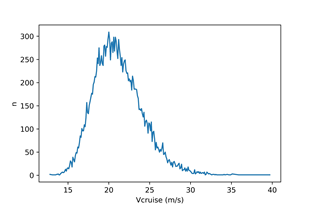
\includegraphics[width=\textwidth]{cruise-velocity-distribution}
        \caption{Velocity}
        \label{fig:cruise-distribution:velocity}
    \end{subfigure}
    \hfill
    \begin{subfigure}[b]{0.49\columnwidth}
        \centering
        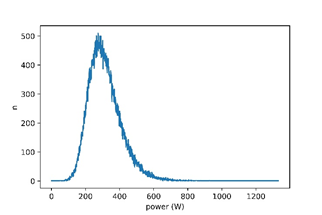
\includegraphics[width=\textwidth]{cruise-power-distribution}
        \caption{Power}
        \label{fig:cruise-distribution:power}
    \end{subfigure}

    \caption{expected distribution of selected properties during cruise.}
    \label{fig:cruise-distribution}
\end{figure}

We find that the mean value of the power required in cruise is 315W, with a median of 302W, giving an estimated power requirement in cruise of around 310W.
There is more uncertainty with this than with the cruise speed due to the larger range of values covered within one standard deviation of the mean, however this still provides a good starting point for the project.

\subsection{Further constraint analysis} \label{sec:design-process:initial-designs:further-constraint-analysis}

Using the refined parameters found in the initial constraint analysis, design decisions made, and further analysis of the UAV, the constraint analysis can be combined to show all parts of the flight profile to find the minimum power requirement.
This code gives more refined estimates for the power requirement in different areas of the flight envelope, as well as take-off speed.
This can be updated quickly and easily as design decisions are made and various operational parameters are refined.
Figure 5 shows the final plots after all research and design decision were made.

\importimage{full-constraint-analysis}{full constraint analysis plot with feasible region highlighted.}{Full constraint analysis}{0.85}
\importimage{takeoff-speed-plot}{takeoff speed plot.}{Takeoff speed plot}{0.85}

It can be seen that the lowest thrust to weight ratio required is around 0.29, which corresponds to a power requirement of around 520W, however this is for a wing loading of only 100N/m2.
The final wing loading of ELMO UAV turned out to be approximately 111N/m2, giving a thrust to weight requirement of just over 0.3 and a corresponding power requirement of around 650W, and so the final selection of motors is sufficient with a small amount of power to spare. 

\subsection{Wing} \label{sec:design-process:initial-designs:wing}

Early in the project, due to its nature: the complexity of certain components and the limited budget, it was decided that a simple rectangular wing would be used on the UAV.
Taking the modularity onto account, a rectangular wing would reduce the possible number of engine housing units needed, therefore reducing the amount of design and manufacturing, and therefore cost of the project. 

The UAV had a 2m span, with a fixed chord of 30cm, which gave an aspect ratio of 6.6.
The chord length was initially at 25cm, closer to the desired aspect ratio of 8.
However, concerns regarding the size of flaps and ailerons were raised as a significant amount of the wingsipan would be lost to the motor housing units, so the chord length was increased to 30cm as a compromise.  

Once a wing shape had been decided a more detailed analysis of possible airfoil sections took place.
Initial 2D simulations were run on XFLR (XFLR, 2019) to narrow the choice down to five airfoils.
The analysis was run at a Reynolds number of $1.35x10^6$, calculated using standard atmospheric conditions at a cruise speed of 20m/s and a reference length on XFLR of 1m. 

Although the purpose of the project is to improve the efficiency of electric aircraft by altering the position of the propulsion units, the aim is not to produce the most efficient aircraft, but more a test craft which can be reused.
Therefore, when choosing the airfoil the main considerations where not only L/D but also stall angle, max Cl and moment coefficient amongst others.
The analysis narrowed down to four potential airfoils: The Clark Y, S1223, NACA6412, RG15A213, whose coordinates were taken from (Tools, 2019) Figures 1a,b, and c  show the Cl-alpha, Cl/Cd, and Cm – alpha curves respectively of four suitable airfoils. 

The Clark Y (blue line) is very common among model UAV makers because of its gentle stall angle at around 12 degrees, with a further sharper drop off at around 20degrees.
It also has a gentle moment coefficient which makes it stable to changes in attitude during flight. 

The S1223 (black line) has an extremely high L/D ratio due to its high camber, it also has a slightly higher stall angle than the Clark Y (at around 14 degrees).
However, it has an unfavourably large moment coefficient, which may make it unstable in flight.
Its high camber and narrow trailing edge may also make it difficult to implement high lift devices as well as it not being strong enough to support a tractor propulsion set up. 

The NACA6412  (green line) has a high L/D ratio up to 10degrees of incidence as well as a higher Cl-alpha curve which is useful as a large part of the wing wetted area will be taken by motor housing.
However, it has a slightly higher moment coefficient than the Clark Y at low angle as well a lower, yet gentle, stall angle of 11 degrees.

The RG15A213 (red line) has the lowest Cl – alpha of the five, but has a higher stall angle at 15 degrees as well as having the lowest moment coefficient.

Of the five airfoils above, further analysis would be carried out on the Clark y and the NACA6412 airfoils as they provided good lift performance, strong lift to drag ratio and a manageable moment coefficient.

\importimage{alpha-characteristics}{variation of $C_L$, $C_L/C_D$, and $C_M$ with $\alpha$.}{Angle of attack characteristics}{0.9}

\subsection{Fuselage} \label{sec:design-process:initial-designs:fuselage}

This project is designed with the intention of using electric propulsion on commercial aircraft in the future.
Therefore, the design of the UAV was based around commercial aircraft, this discounted any lightweight or double fuselage seen on many UAV’s such as SPOTTER (SPOTTER, 2019). 

Initial designs included a square, circular and airfoil shaped fuselage.

\importtable{| >{\raggedright\arraybackslash}p{0.12\columnwidth} | >{\raggedright\arraybackslash}p{0.36\columnwidth} | >{\raggedright\arraybackslash}p{0.36\columnwidth} |}{
    \hline
    \textbf{Design} & \textbf{Advantages} & \textbf{Disadvantages} \\
    \hline
    Square & Easy manufacturing and wing attachment; strong structural performance & Poor aerodynamics \\
    \hline
    Circular & Easy to manufacture & Hard to attach wing; difficult to create internal structure \\
    \hline
    Aerofoil & Aerodynamic; aesthetically pleasing & Difficult to manufacture \\
    \hline
}{tradeoffs involved in the type of fuselage design.}{fuselage-tradeoffs}

\importimage{potential-aerofoil-design}{potential aerofoil fuselage design.}{Potential aerofoil design}{0.5}

For the wind tunnel model, it was decided that a hybrid of a square fuselage and an airfoil shaped fuselage would be beneficial.
It was thought that a side profile of a NACA0012 airfoil would reduce drag and increase lift, whilst a square front section would make manufacturing easier.
This would give a combination between an aerodynamic design and ease of manufacturing.  

The NACA0012 was chosen as a suitable airfoil as it would provide enough height to hold all the electronics, as well as enough room to reach in in case needed. 

The initial fuselage design was 1.5m long, with a width of 175mm and a height (at the thickest part) equal to around 180mm. 

\subsection{Tail} \label{sec:design-process:initial-designs:tail}

Note, for many of the tail and control surface mathematical design processes, details of the equations used are unnecessary for understanding, but for the interested reader, they can been seen in the appendices, and appropriately headed and labelled. 

The tail was designed with a volume coefficient process.
First, volume coefficients were estimated from Raymer’s book: ‘Aircraft design: A conceptual approach’, table 9.4 (Raymer, 1989), and a value of 0.8 was selected for the horizontal, and 0.07 for the vertical tail volume.
Next values for tail surface aspect ratios were estimated as 5 for the horizontal tail, and 2 for the vertical tail from table 9.1 in (Raymer, 1989).
The formulae for vertical and horizontal tail volume coefficients for tailplane areas were rearranged to obtain the vertical and horizontal tail areas, where then the aspect ratio selected could be used to determine span, and then MAC of the tail surfaces.
Lastly the taper ratio was used to determine root and tip chords of the tail surfaces.
At this stage, no setting angle was determined as the need for this had not been recognised. 

Next, the spars had to be sized for the wind tunnel test.
We were advised by our supervisor, Prof. Keith Towell to size them for 10g loads (Towell, 2019).
A simple mathematical beam model was used to size the spars in the tail as well as the main structural arm.
The horizontal tail spars were modelled as having a 5g (49.05N) load distributed evenly over the semi span.
Based on values for the inner and outer diameters of the spars, length and chosen material stiffness, the tip deflection was found.
The main structural arm was determined by modelling a 10g point load in line with the horizontal spars, and using inner and outer widths instead of diameters, as it was decided this would be a square section to prevent parts rotating around it.

\subsection{Control surfaces, electronics, and avionics} \label{sec:design-process:initial-designs:control-surfaces-electronics-and-avionics}

The initial design was with the first wind tunnel test in mind, and as such made no plans for functional control surfaces, electronics or avionics at this point.
It was hoped that the first test would ‘nail down’ the basics of the fuselage, wing and tail geometry, or show us where changes would be required from our initial design, and subsequent models and tests could validate the performance of more complex aspects of the design and performance of the UAV. 

\subsection{Propulsion} \label{sec:design-process:initial-designs:propulsion}

\subsubsection{Twist-in motor attachment} \label{sec:design-process:initial-designs:propulsion:twist-in-motor-attachment}

\begin{figure}[H]
    \centering
    \begin{subfigure}[b]{0.49\columnwidth}
        \centering
        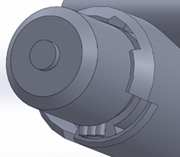
\includegraphics[width=\textwidth]{twist-in-in-place}
        \caption{Motor in-place in housing}
        \label{fig:twist-in:in-place}
    \end{subfigure}
    \hfill
    \begin{subfigure}[b]{0.49\columnwidth}
        \centering
        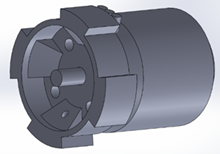
\includegraphics[width=\textwidth]{twist-in-attached}
        \caption{Bracket attached to motor}
        \label{fig:twist-in:attached}
    \end{subfigure}

    \begin{subfigure}[b]{0.49\columnwidth}
        \centering
        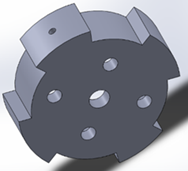
\includegraphics[width=\textwidth]{twist-in-bracket}
        \caption{Bracket}
        \label{fig:twist-in:bracket}
    \end{subfigure}
    \hfill
    \begin{subfigure}[b]{0.49\columnwidth}
        \centering
        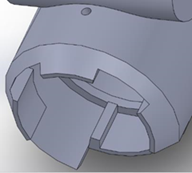
\includegraphics[width=\textwidth]{twist-in-housing}
        \caption{Housing}
        \label{fig:twist-in:housing}
    \end{subfigure}
    \caption{CAD models of the twist-in motor attachment used in the tail.}
    \label{fig:twist-in}
\end{figure}

Designed early on in the project this was a proposed design for the attachment of the wing motors, however when the design criteria changed to include a battery and ESC in the movable propulsion unit, a new design was required.
However, this design is still used in the tail location as the battery and ESC are fixed in the fuselage for that configuration, and so only the motor moves making this an ideal solution.
The design is intended to allow for very quick and simple removal and replacement of the motor when changing configurations of the UAV in order to reduce ground time at the flying days.
This utilises a twist and fix design where four tabs on the bracket, shown in Figure 1 c), which attaches to the back of the motor as shown in Figure 1 b), engage with four tabs in the housing and the motor then rotates up to a limiting piece to align the bracket and housing, shown in Figure 1 d) and a).
The motor is then secured in place using a small grub screw which engages with the bracket through a clearance hole in the top of the housing, as shown in Figure 1 d), providing the resistance to rotation of the motor while the tabs provide the strength in the direction of the force of the motor.
The large cut-out in the housing, shown in Figure 1 d), is to allow room for the wires of the motor when it is being fitted, as they protrude from the rear part of the motor out to the side, shown in Figure 1 a).
On the final design for the tail there is a full routing designed for the wires but that is was not designed here as this housing was intended for the wing, but then not used.

\subsubsection{Sizing} \label{sec:design-process:initial-designs:propulsion:sizing}

Initial sizing started from the constraint analysis power requirement estimations, allowing motors to be selected.
The constraint analysis at this point was suggesting a power requirement of around 600W, and so motors were researched of around this power from a recommended supplier Outlander, and a number of suitable cost effective motors were found for both the fuselage and wing locations, as listed in Figure 1 a).
These were then used to find suitable ESCs, which were recommended for the motors as 60A and 30A, but due to this being the most common part to fail on previous projects due to overloading, a decision was made to oversize the ESCs by 30\% and so 40A and 80A ESCs were selected.
The batteries were then chosen based on the voltage and current requirements of the motors, meaning that they needed to be 4S to provide the required 14.8V, and the capacity initially chosen simply on weight and cost, with the largest capacity shown being the heaviest we could use.
The C value is used to find the max current output of the battery and so this was chosen to ensure a large safety margin between the max of the battery and the max of the motor to reduce any chance of overheating of the battery while in use. 

The motor selection was then refined due to an increase in the power requirement prediction from the constraint analysis due to confirmations in the UAV design, this meant that the motors could be selected as the Tornado Thumper V3 3548/05 and 3530/14 for the fuselage and wing motors respectively.
This meant that the battery capacities could be checked for time of flight based on an estimated 75\% throttle average throughout a flight, this is an overestimate but gives a useful pessimistic estimation of the flight time.
This showed that the smaller capacity batteries would not be enough to provide a suitable flight time in order to record the data we would need while having a margin in the battery to avoid a power cut-out mid-flight.
Along with finalising the battery selection, the propellers could now be researched as shown in Figure 1 b).
This initially required the maximum propeller diameter to be found for the motors, based on the max rpm of the motor, which would give a tip Mach No of the propeller of around 0.7 which would maximise thrust without having large increases in power requirement due to transonic effects at the blade tip.
This was then used to refine an iterative search of the available propellers from APC, a trusted manufacturer by the University.
The advance ratio was found based on the blade diameter, RPM, and a target max flight speed of 25m/s, and then a suitable propeller found in the database that had a power draw similar to that of the max of the motor at the target flight speed and RPM, while providing enough thrust based on estimations of the aircraft drag.
These propellers were then checked after selection at the target cruise speed of 20m/s to ensure that the thrust would be adequate, and to find an estimation of the efficiency in order to further refine the constraint analysis.
The ideal propellers, however, could not be used due to the specific use case of the project, which requires both tractor and pusher configurations to be employed, as well as counter rotating propellers on each wing, and this meant that the propeller would need to have an equivalent pusher propeller.
This meant that the selection of propellers was forced into non-ideal blades, with the fuselage propeller only having one viable option of the APC 12x6E and 12x6EP propellers, and the wing having two options of the 8x6E and 7x5E, which after analysis of thrust data, the 8x6E was chosen to be used in a motor and propeller wind tunnel test to verify that this propeller would be suitable, and to verify the quoted performance data in order to ensure that the 12x6E would also be suitable. 

\section{Interim design review} \label{sec:design-process:interim-design-review}

\subsection{Wind tunnel test} \label{sec:design-process:interim-design-review:wind-tunnel-test}

\subsubsection{Fuselage} \label{sec:design-process:interim-design-review:wind-tunnel-test:fuselage}

The fuselage was designed around a hollow 1m long and 20mm square aluminium boom as its core structural element.
Around the boom was a foam and poplar plywood structure, similar to the wing. 

The driving force behind the fuselage design was the need to be able to change the setting angle of the wing with ease.
As a result, the metal boom was fixed to four layers of poplar ply ribs which ran the length of the fuselage. 

To allow the wing setting angle to be changed easily three sets of holes ran through the fuselage.
The front hole was a tight fir for the front spar, so it didn’t move.
The middle was a guide for the rear spar to help changing the angle.
The rear set of holes were to secure the wing in place.
This section contained seven holes in total, each 2 degrees apart, meaning the wings angle could be changed form 0 degrees up to 12 degrees. 

\importimage{fuselage-cross-section}{a cross-section of the fuselage, showing the structure and hole layouts.}{Fuselage cross-section}{0.6}

At the rear of the model, on the underside, the middle two ribs contained an attachment point for the wind tunnel.
This was extruded from the model to enable the model to be easily attached and removed from the struts. 

\importimage{laser-cut-plywood}{laser-cut plywood for the fuselage.}{Laser-cut plywood}{0.7}

\subsubsection{Wing} \label{sec:design-process:interim-design-review:wind-tunnel-test:wing}

The wing was constructed using two hollow aluminium spars as the key structural element.
The front spar at quarter chord, the rear spar at half chord, with outer diameters of 15.88mm and 12.7mm, respectively.
Each spar was 2m long and ran tip to tip through the fuselage.
Surrounding the spars was blue Styrofoam, cut from the university foam cutter.
Separating the foam sections were 3mm thick poplar ply ribs, cut on university laser cutter.
Each rib had a unique design and were individually designed and cut.

\importimage{flap-dfx-file}{DFX file of flap rib for the Clark Y aerofoil section, later used for laser cutting.}{Flap DFX file}{0.6}

There were 6 ribs used in each wing half, in locations that would roughly replicate where the motor housing units would be on the final model.
Therefore, the ribs were located either side of the flap and 130mm outboard.
The next rib, located 101mm outboard, was the rib used to connect the model to the wind tunnel.
Therefore, it was made from 6mm birch ply as this provided enough strength to an integral component.
The two final ribs were located at the wing tip and 50mm inboard.

\importimage{underside-of-wing}{the underside of the wing, showing attachment and flap adjustment methods.}{Underside of wing}{0.6}

The thicker birch ply rib, located 700mm outboard of the centre of the aircraft, contained an extrusion with a hole for a M6 bolt to allow easy attachment and removal to the wind tunnel mounts.
It was located at 700mm from the centre of the fuselage as dictated by the wind tunnel capabilities. 

The foam and ribs for each side of each wing were bonded together using epoxy resin but were not bonded to the spars themselves.
This was to allow the wing sections to be removed from the spars during the wind tunnel test. 

The wings were secured to the wing using two 3D printed clamps on each spar. 

\importimage{internal-spar-structure}{Wing section showing the internal spar structure.}{Internal spar structure}{0.6}

\subsubsection{Control surfaces} \label{sec:design-process:interim-design-review:wind-tunnel-test:control-surfaces}

The main purpose for the wind tunnel model was to cement top level parameters such as airfoil section, setting angle, chord length and wingspan.
As a result, the wind tunnel was unpowered, and ailerons not included in the model.
However, it was important to test the effect of a flap on each wing and which airfoil would be more suitable to the addition of a flap. 

Initial research stated that, for a typical low speed UAV, ailerons take up approximately 40\% of the semi-span, in this case 400mm (Sadraey, 2013).
This left the remaining 60\% for flaps.
However, the design at the time was for the motor housing units to have width of approximately 110mm.
There would be two located on each half of the wing, plus a tip mounted motor as well, which had an unknown depth at the time.
Therefore, the flaps were set to a width of 380mm, which would act as a “worst case scenario” approach to the design and would provide each wing section with a strong test. 

The flaps were designed to be changed manually, whilst the model was still attached to the wind tunnel.
The guided either side of the flaps had M2 holes every 5 degrees up to 35 degrees.
As the flap was altered two M2 bolts would secure the flap in place. 

\importimage{flap-mechanism}{close up of the flap mechanism.}{Flap mechanism}{0.6}

\subsubsection{Tail} \label{sec:design-process:interim-design-review:wind-tunnel-test:tail}

With the mathematical modelling complete, a 3D model of the tail surfaces could then be created as reference for building.
This was done by defining the sketch planes that the roots and tip chord aerodynamic profiles would be created on, importing curves of the aerofoil from coordinate files and parametrizing them (chord length and angle of attack) so that they could be manipulated.
Lofted bases were created between the profiles, then additional details such as cut-outs for spars were added.
This was repeated for all three control surfaces, and then simple models of the tail spars and main structural arm created and added to the overall assembly. 

The initial plan was to use the foam cutter to create the tail profiles, however, this proved to be infeasible as the cut-outs for the spars in a thin aerofoil profile (NACA0012) left very little foam in the wall which resulted in the foam melting at the tip where the cutter had to slow down.  

There wasn’t time to redesign the tail because of the upcoming test, so it was decided to laser cut profiles at equally spaced intervals along the tail surfaces and wrap Solarfilm around it.
Geometry was created in CAD using repeated 3mm profiles intersecting the foam geometry, and then non-intersecting geometry deleted to leave the laser cut profiles, which were quickly exported and cut.
Each profile was mounted and bonded to the spar.
Once the glue had cured, Solarfilm was wrapped around the profiles, with the leading and trailing edges stiffened with card.
This was messy but worked, while we resolved to refine the model for the next iteration of the design.  

The tail was mounted on the model using a friction fit with the spars running through the fuselage and main structural arm.
Holes were drilled through these that were intentionally a half millimetre short of the spacing required.
One horizontal tail surface was glued to one spar, and the other to the second, so they would slot together neatly in the model.
The vertical tail surface contained both spars, and simply slotted in all at once. 

\importimage{wind-tunnel-model}{final wind tunnel model.}{Wind tunnel model}{0.8}

\subsubsection{Test plan} \label{sec:design-process:interim-design-review:wind-tunnel-test:test-plan}

The wind tunnel test had a few objectives.
The first was to validate the designs produced so far, ensuring that lifting surfaces could produce sufficient lift and were able to withstand the predicted structural loads.
Assuming these conditions were met, a combination of aerofoil, wing-body angle, and flap-wing angle needed to be found which optimised the objective function (discussed later in more detail).
Data collected during this optimisation would also be used afterwards to alter the design further - estimating the change to lift or drag that could be obtained by changing the size of the flaps - and to validate the accuracy of CFD simulations. 

Five variables were controllable within the wind tunnel: aerofoil, angle between the wing and the fuselage (wing-body angle), angle between the flaps at maximum deflection and the wing (flap-wing angle), angle of attack, and airspeed.
The experiment space created by all of these variables is much larger than would have been feasible to explore fully within one wind tunnel session, and so the testing was split into two phases - cruise and takeoff - and some simplifications were made to enable a subset of the experiment space to be explored while still yielding near-optimal results.

During cruise, some of the variables can be fixed.
Angle of attack is set to 0o, cruise speed is fixed at 20 m.s-1, and flaps will not be extended.
The experiment space now consists of the two aerofoil options and a number of wing-body angle settings for each one, but can be reduced further by assuming that an increase in wing-body angle will always correspond to an increase in drag, and will cause an increase in lift as long as the wing has not stalled.
The objective function for the cruise phase of testing can then be defined as the combination of aerofoil and wing-body angle which minimise drag while producing at least 70 N of lift, and then the wing-body angle can be gradually increased for each aerofoil until the lift exceeds 70 N, at which point the testing for that aerofoil is terminated. 

After the cruise phase of testing has been completed, the optimal aerofoil section and wing-body angle can be held constant for the takeoff phase of testing.
If a takeoff speed of 12 m.s-1 is assumed, the experiment can alter the flap-wing angle and angle of attack (to account for bumps or irregularities in the runway) to find a flap-wing angle which maximises L/D while still providing sufficient lift for takeoff at the minimum takeoff angle and not stalling at the maximum takeoff angle.
Reasonable maximum and minimum takeoff angles can be determined from assumptions about the size and length of the landing gear, and the amplitude of bumps on the takeoff surface.
Varying the angle of attack between these two bounds does not cost an excessive amount of time as, unlike the flap-wing angle, that parameter can be varied without the wind tunnel being turned off. 

This procedure was written up into a testing plan, whose conditions enabled the design space to be suitably explored without taking up too much time.
Care was taken to ensure that the plan was objective and covered all edge cases (barring extreme edge cases, such as no configurations producing the required amount of lift or structural failure, which would require a more thorough redesign of the aircraft) so that the results did not need to be discussed during the course of testing.
As much time as possible could then be spent changing to aircraft between the required configurations; estimates of how long would be needed to vary each parameter were also made.

Provisions were also made for gathering some data to analyse the stability of the model if there was any time left over at the end of these two testing phases.
With the optimal aerofoil section, wing-body angle, and flap-wing angle according to the objective functions described above, forces and moments on the model were measured for a range of airspeeds and angles of attack.
Since both of these parameters are variable without turning off the wind tunnel, a relatively large amount of data can be collected fairly quickly.
Once a suitable amount of data were collected, similar sweeps of the parameter space with the optimal configuration would be made with the tail taken off. 

\subsubsection{Results and analysis} \label{sec:design-process:interim-design-review:wind-tunnel-test:results-and-analysis}

\begin{figure}[H]
    \centering
    \begin{subfigure}[b]{0.49\columnwidth}
        \centering
        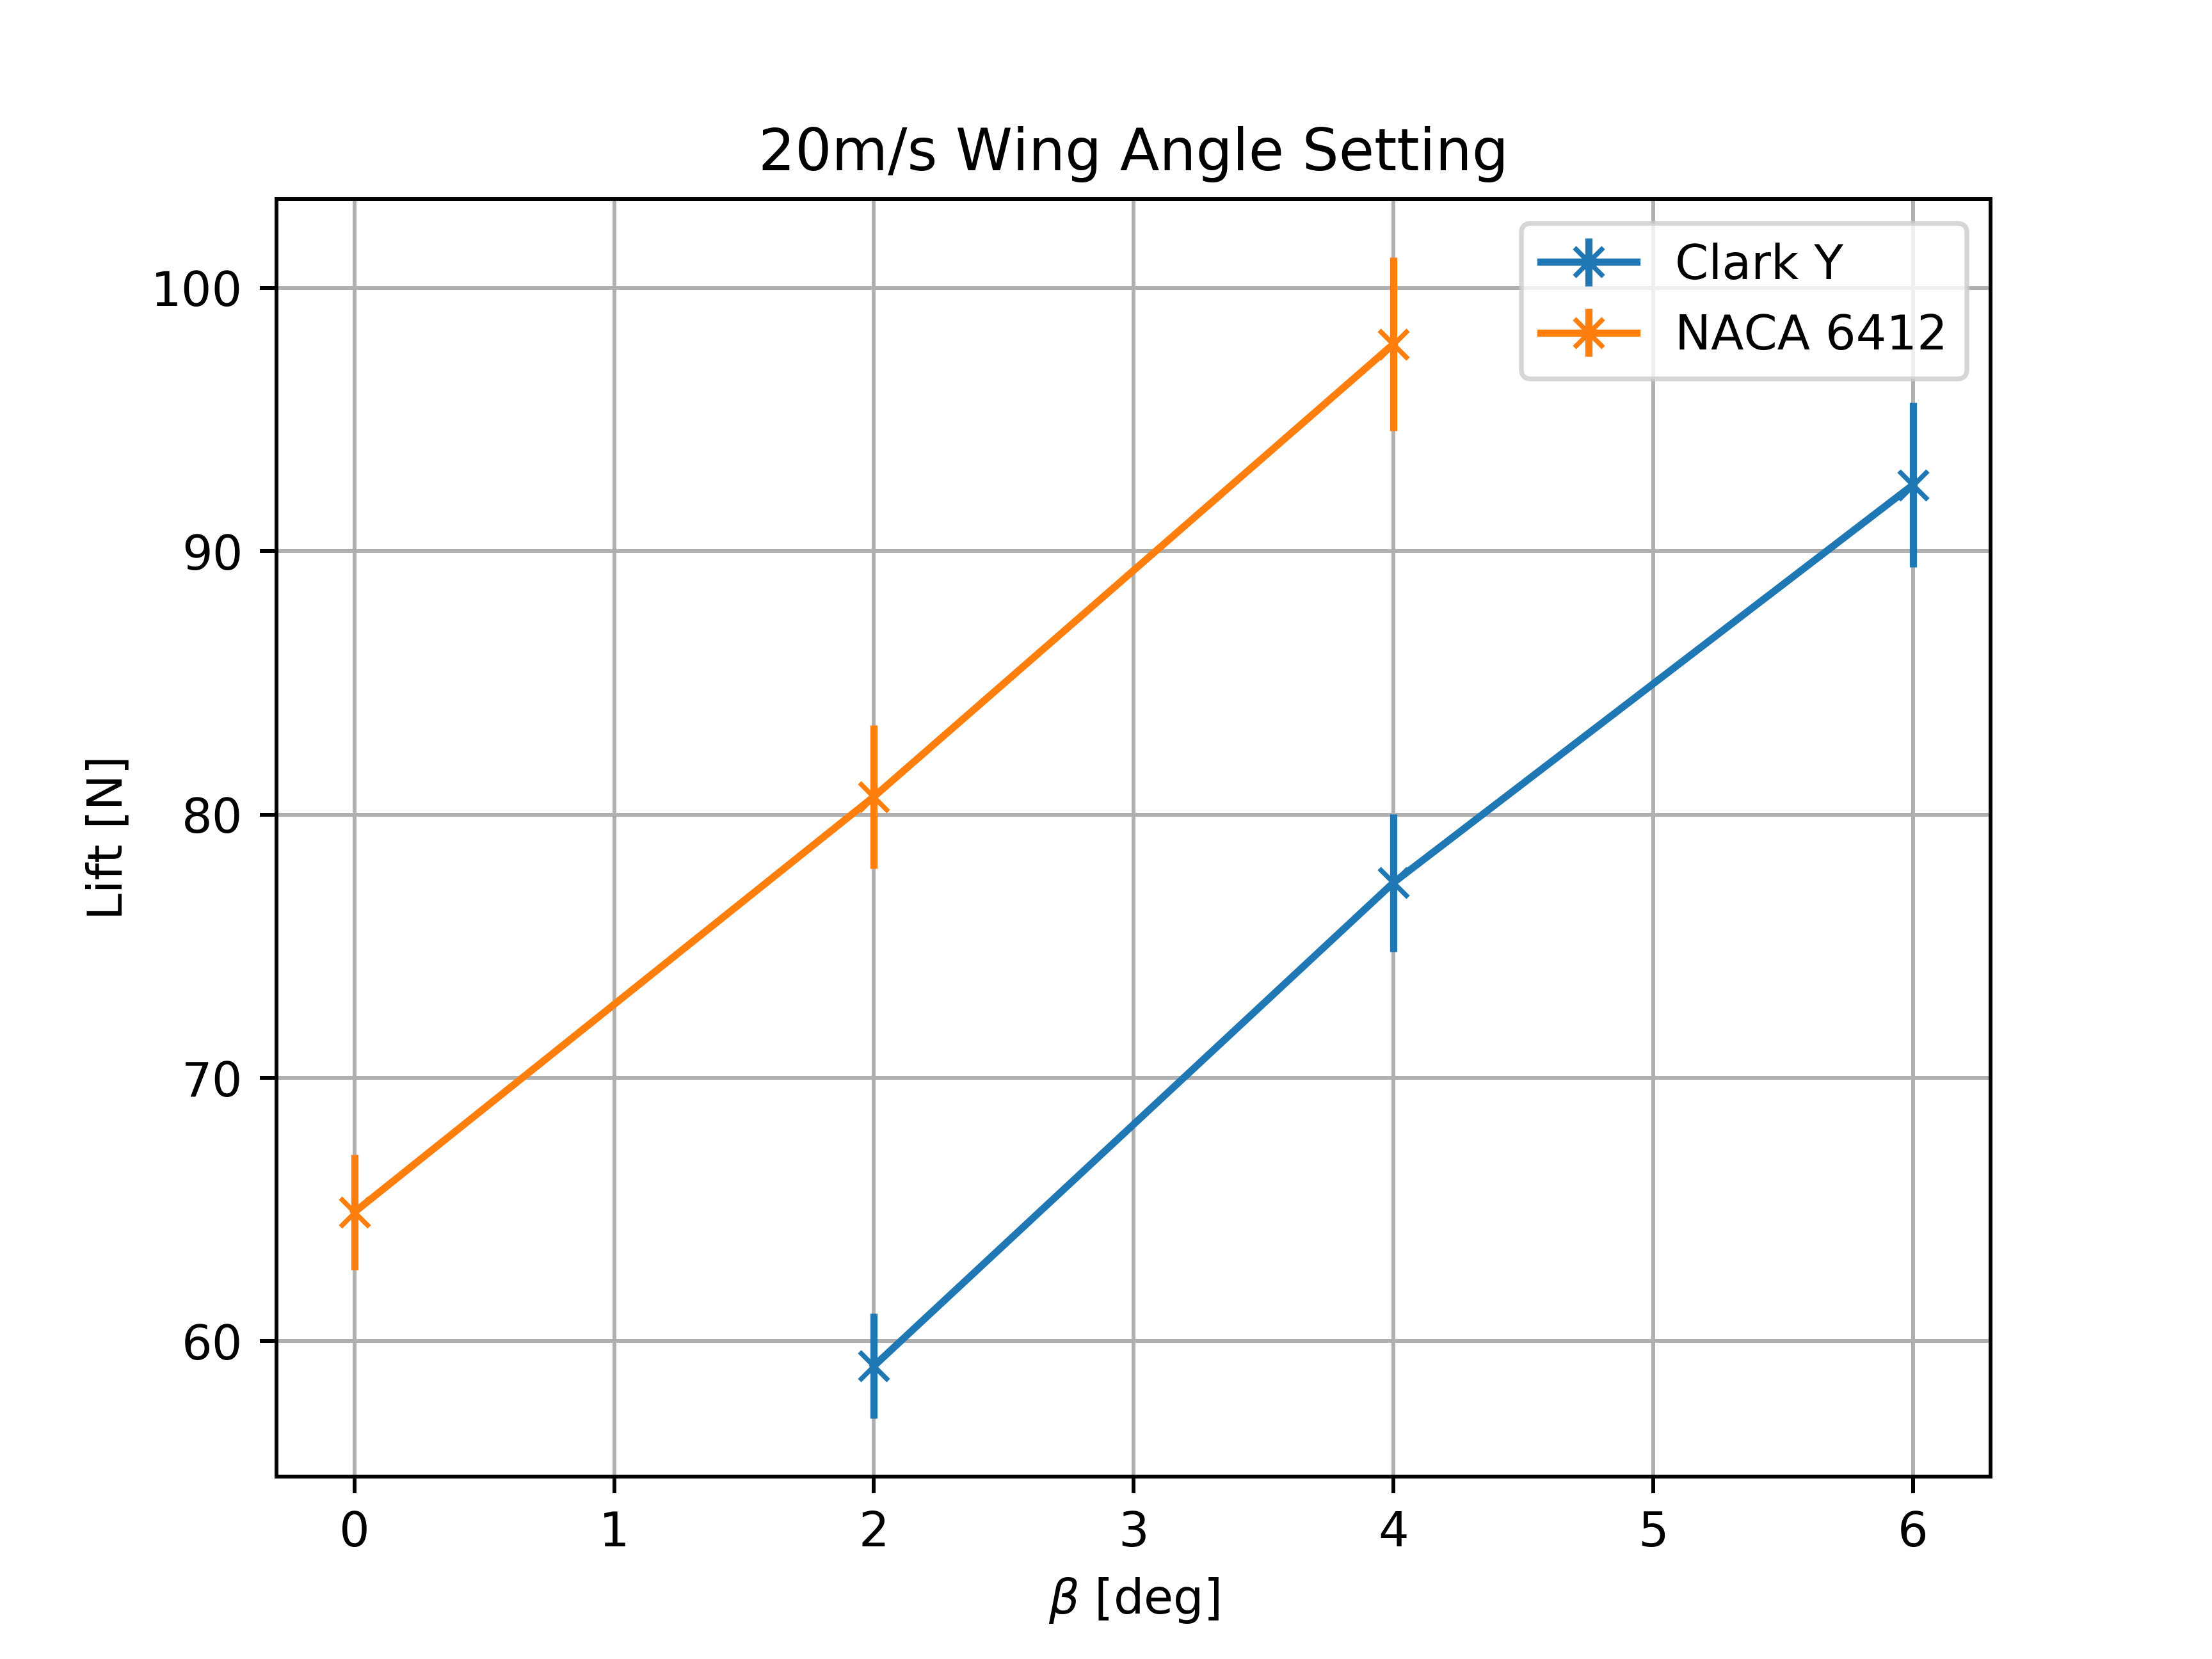
\includegraphics[width=\textwidth]{wing-setting-angle}
        \caption{Wing setting angle}
        \label{fig:wind-tunnel-results:wing-setting-angle}
    \end{subfigure}
    \hfill
    \begin{subfigure}[b]{0.49\columnwidth}
        \centering
        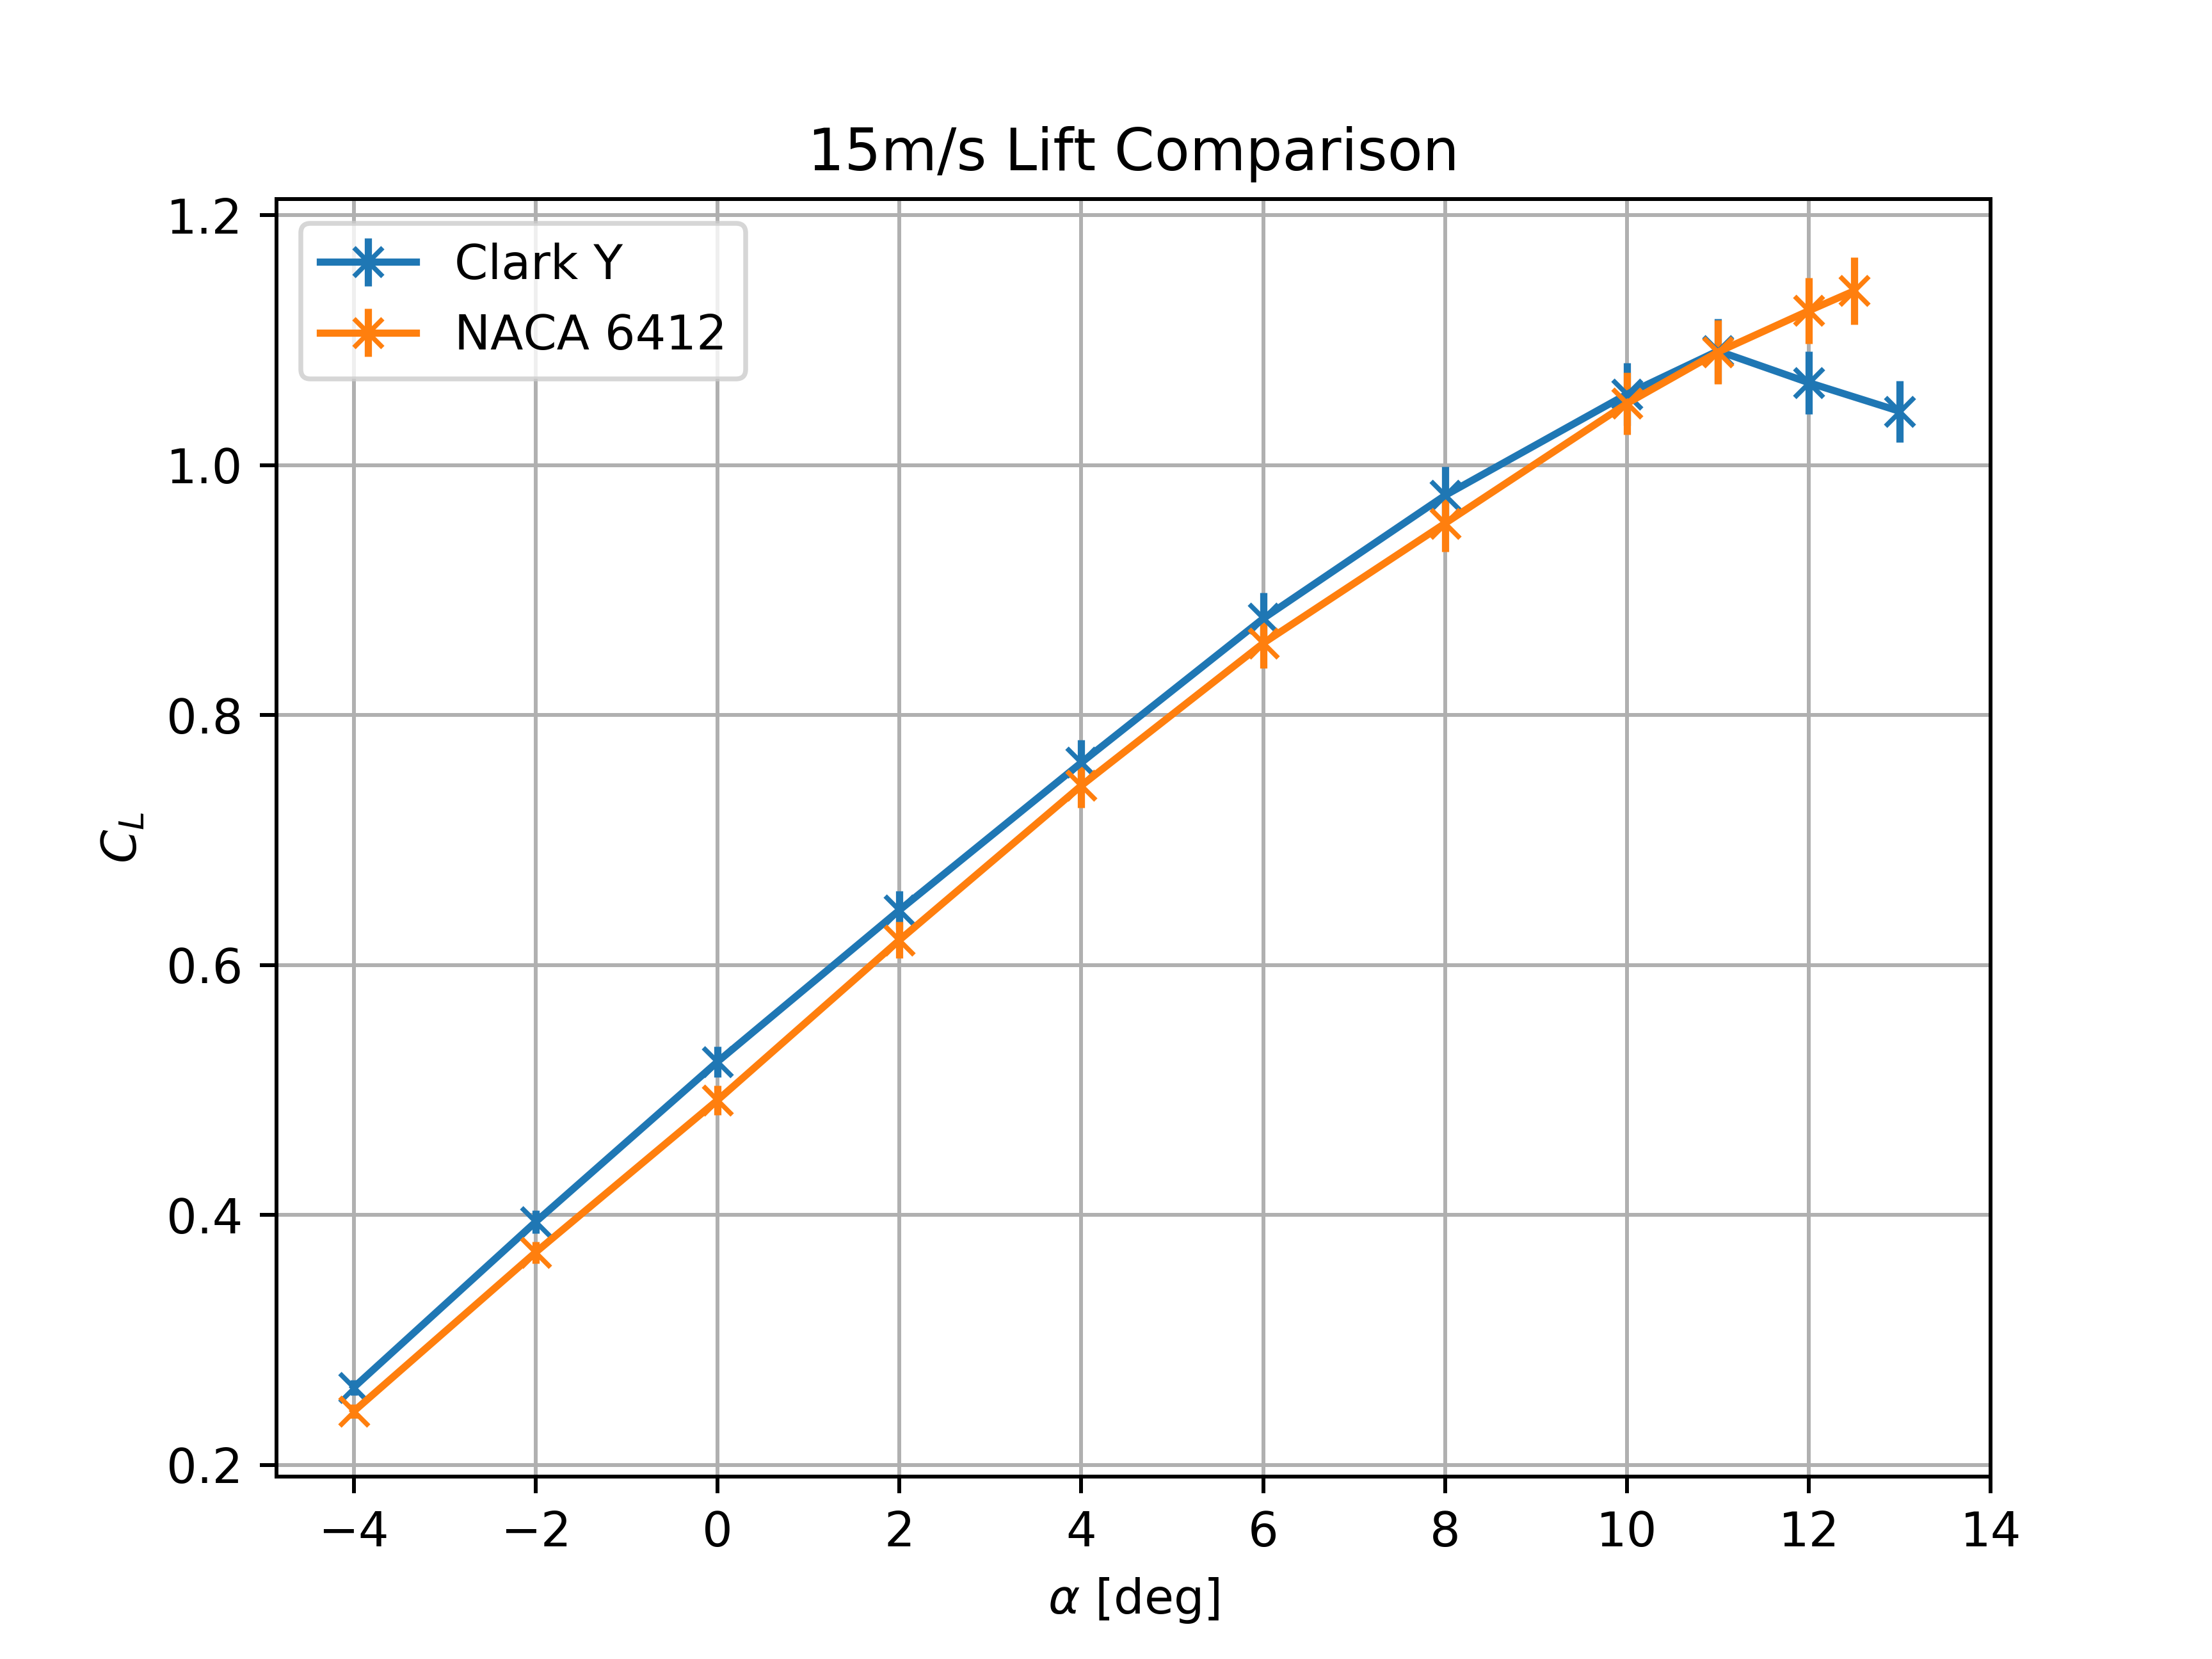
\includegraphics[width=\textwidth]{lift-comparison}
        \caption{Lift comparison}
        \label{fig:wind-tunnel-results:lift-comparison}
    \end{subfigure}

    \begin{subfigure}[b]{0.49\columnwidth}
        \centering
        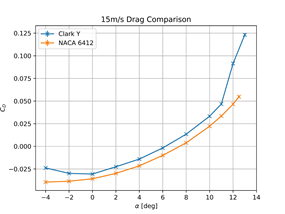
\includegraphics[width=\textwidth]{drag-comparison}
        \caption{Drag comparison}
        \label{fig:wind-tunnel-results:drag-comparison}
    \end{subfigure}
    \hfill
    \begin{subfigure}[b]{0.49\columnwidth}
        \centering
        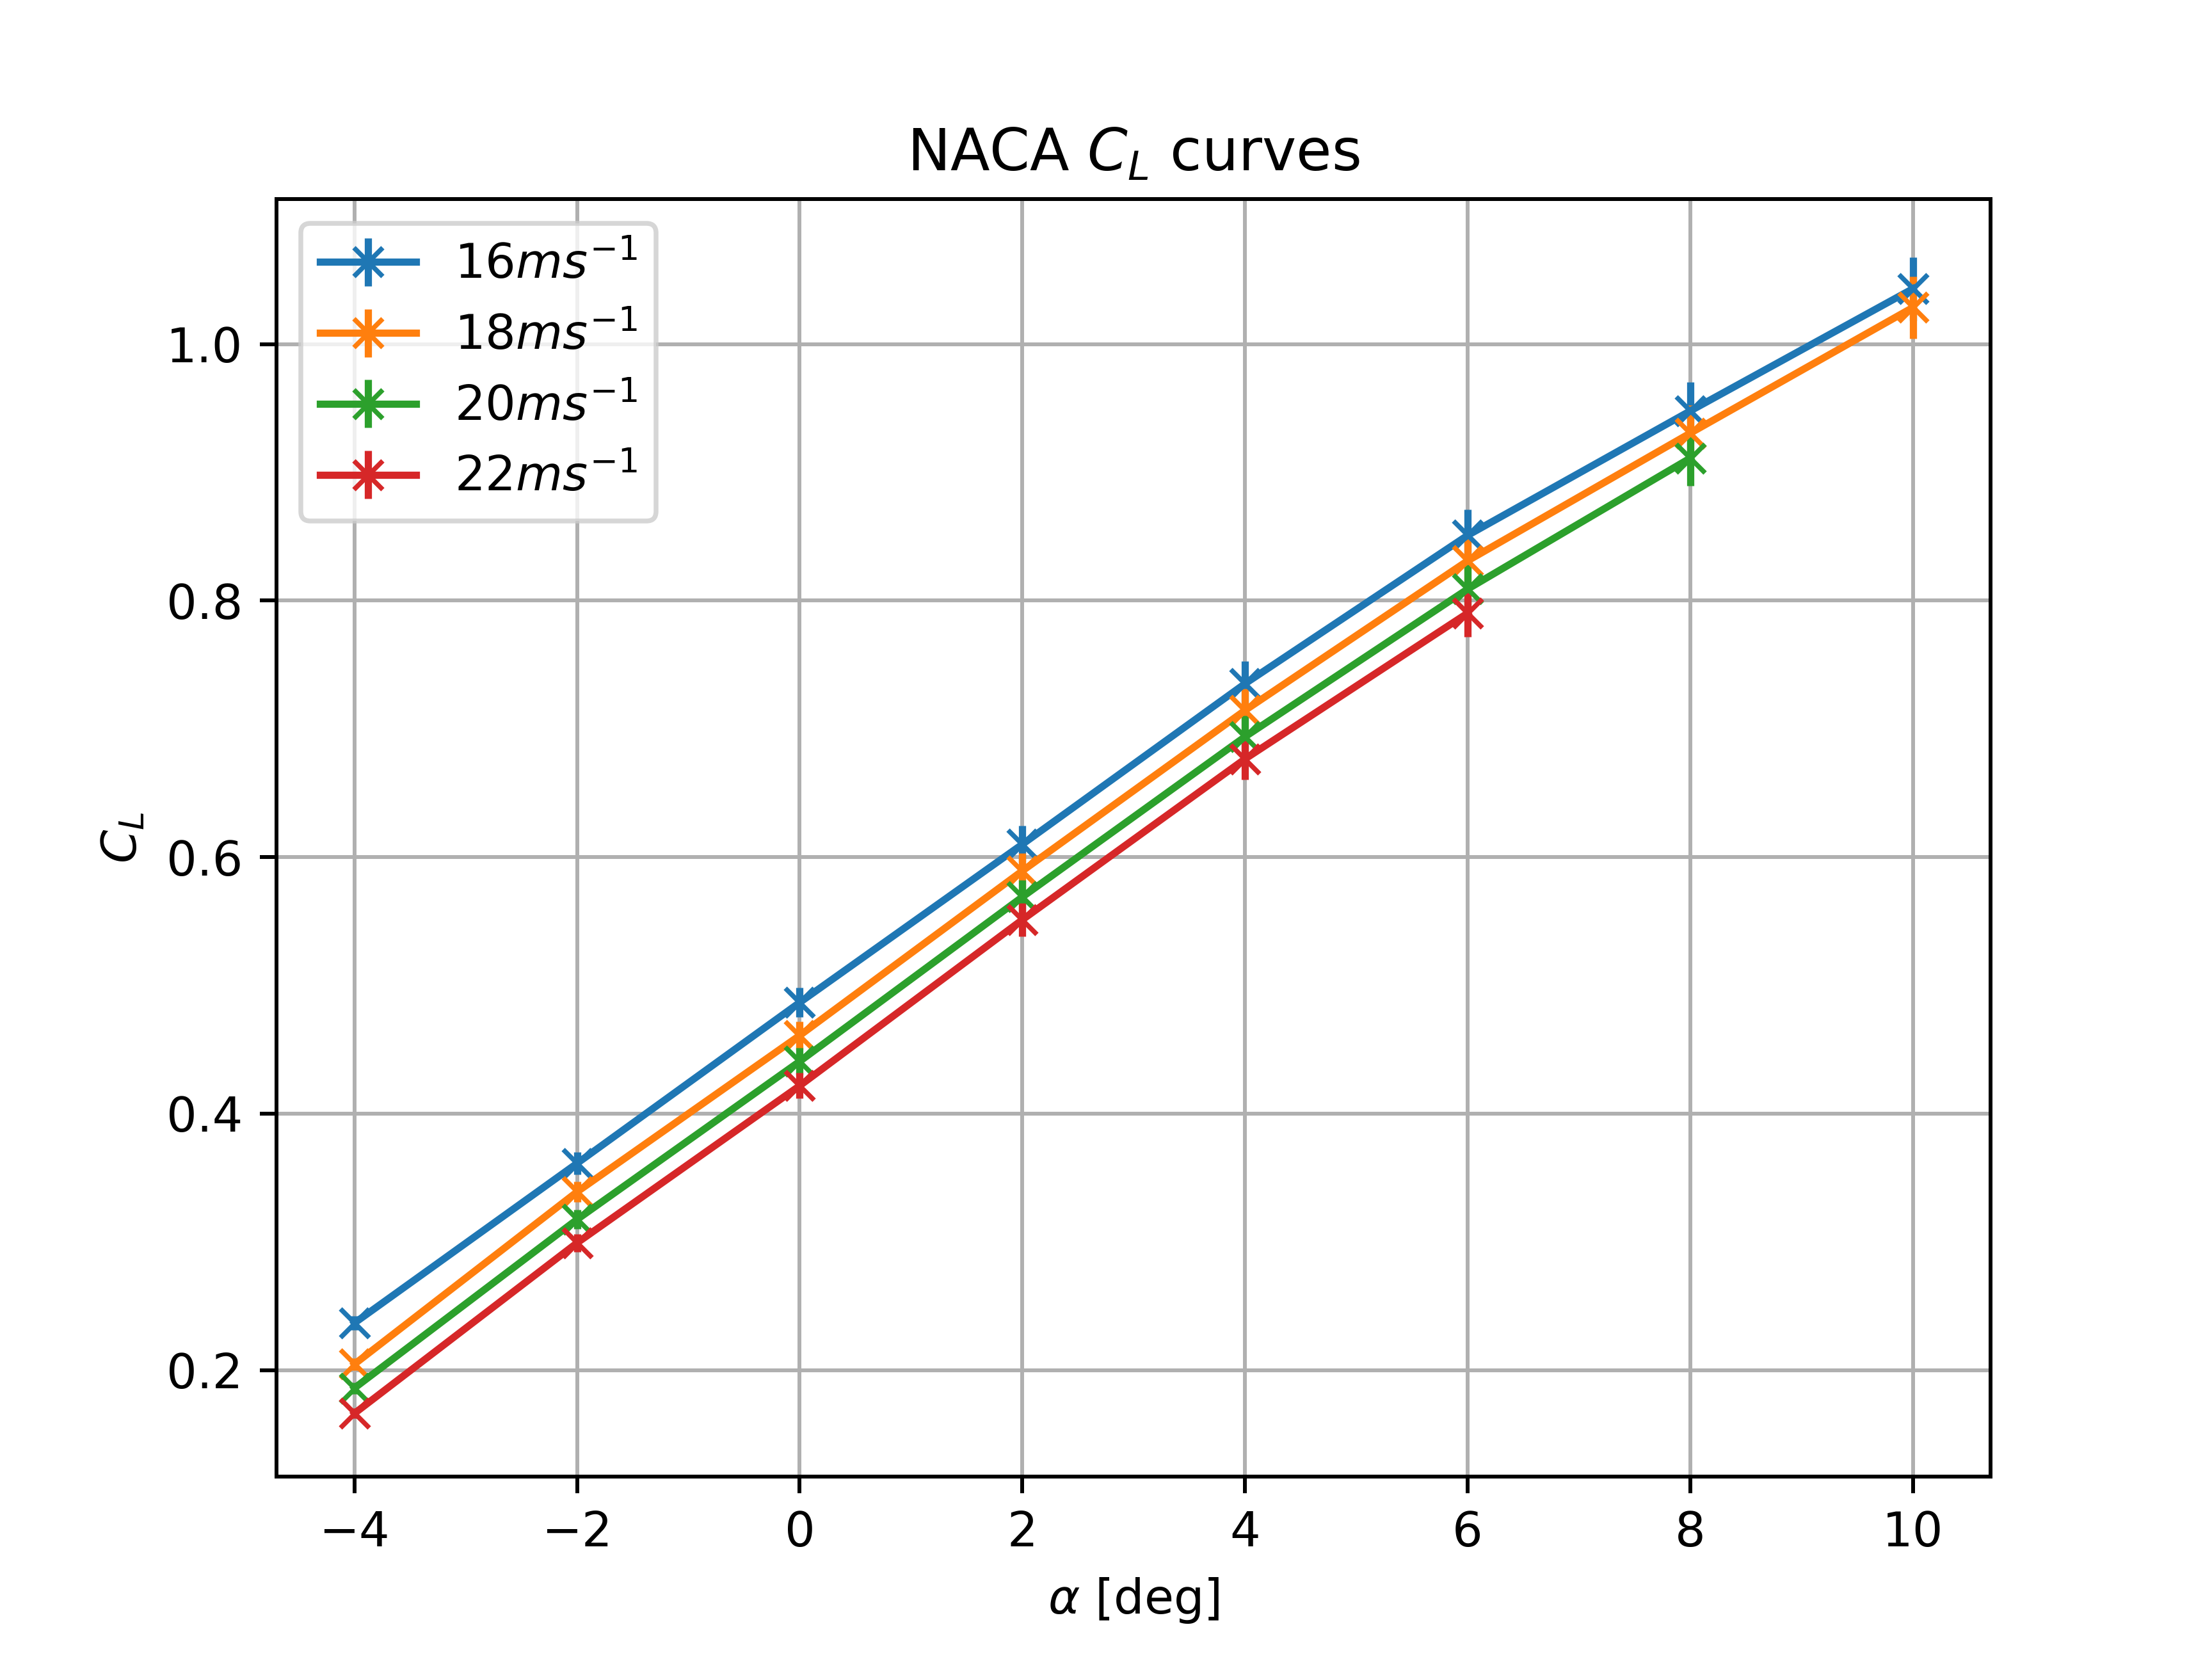
\includegraphics[width=\textwidth]{naca-lift-coefficient}
        \caption{NACA lift coefficient}
        \label{fig:wind-tunnel-results:naca-lift-coefficient}
    \end{subfigure}

    \begin{subfigure}[b]{0.49\columnwidth}
        \centering
        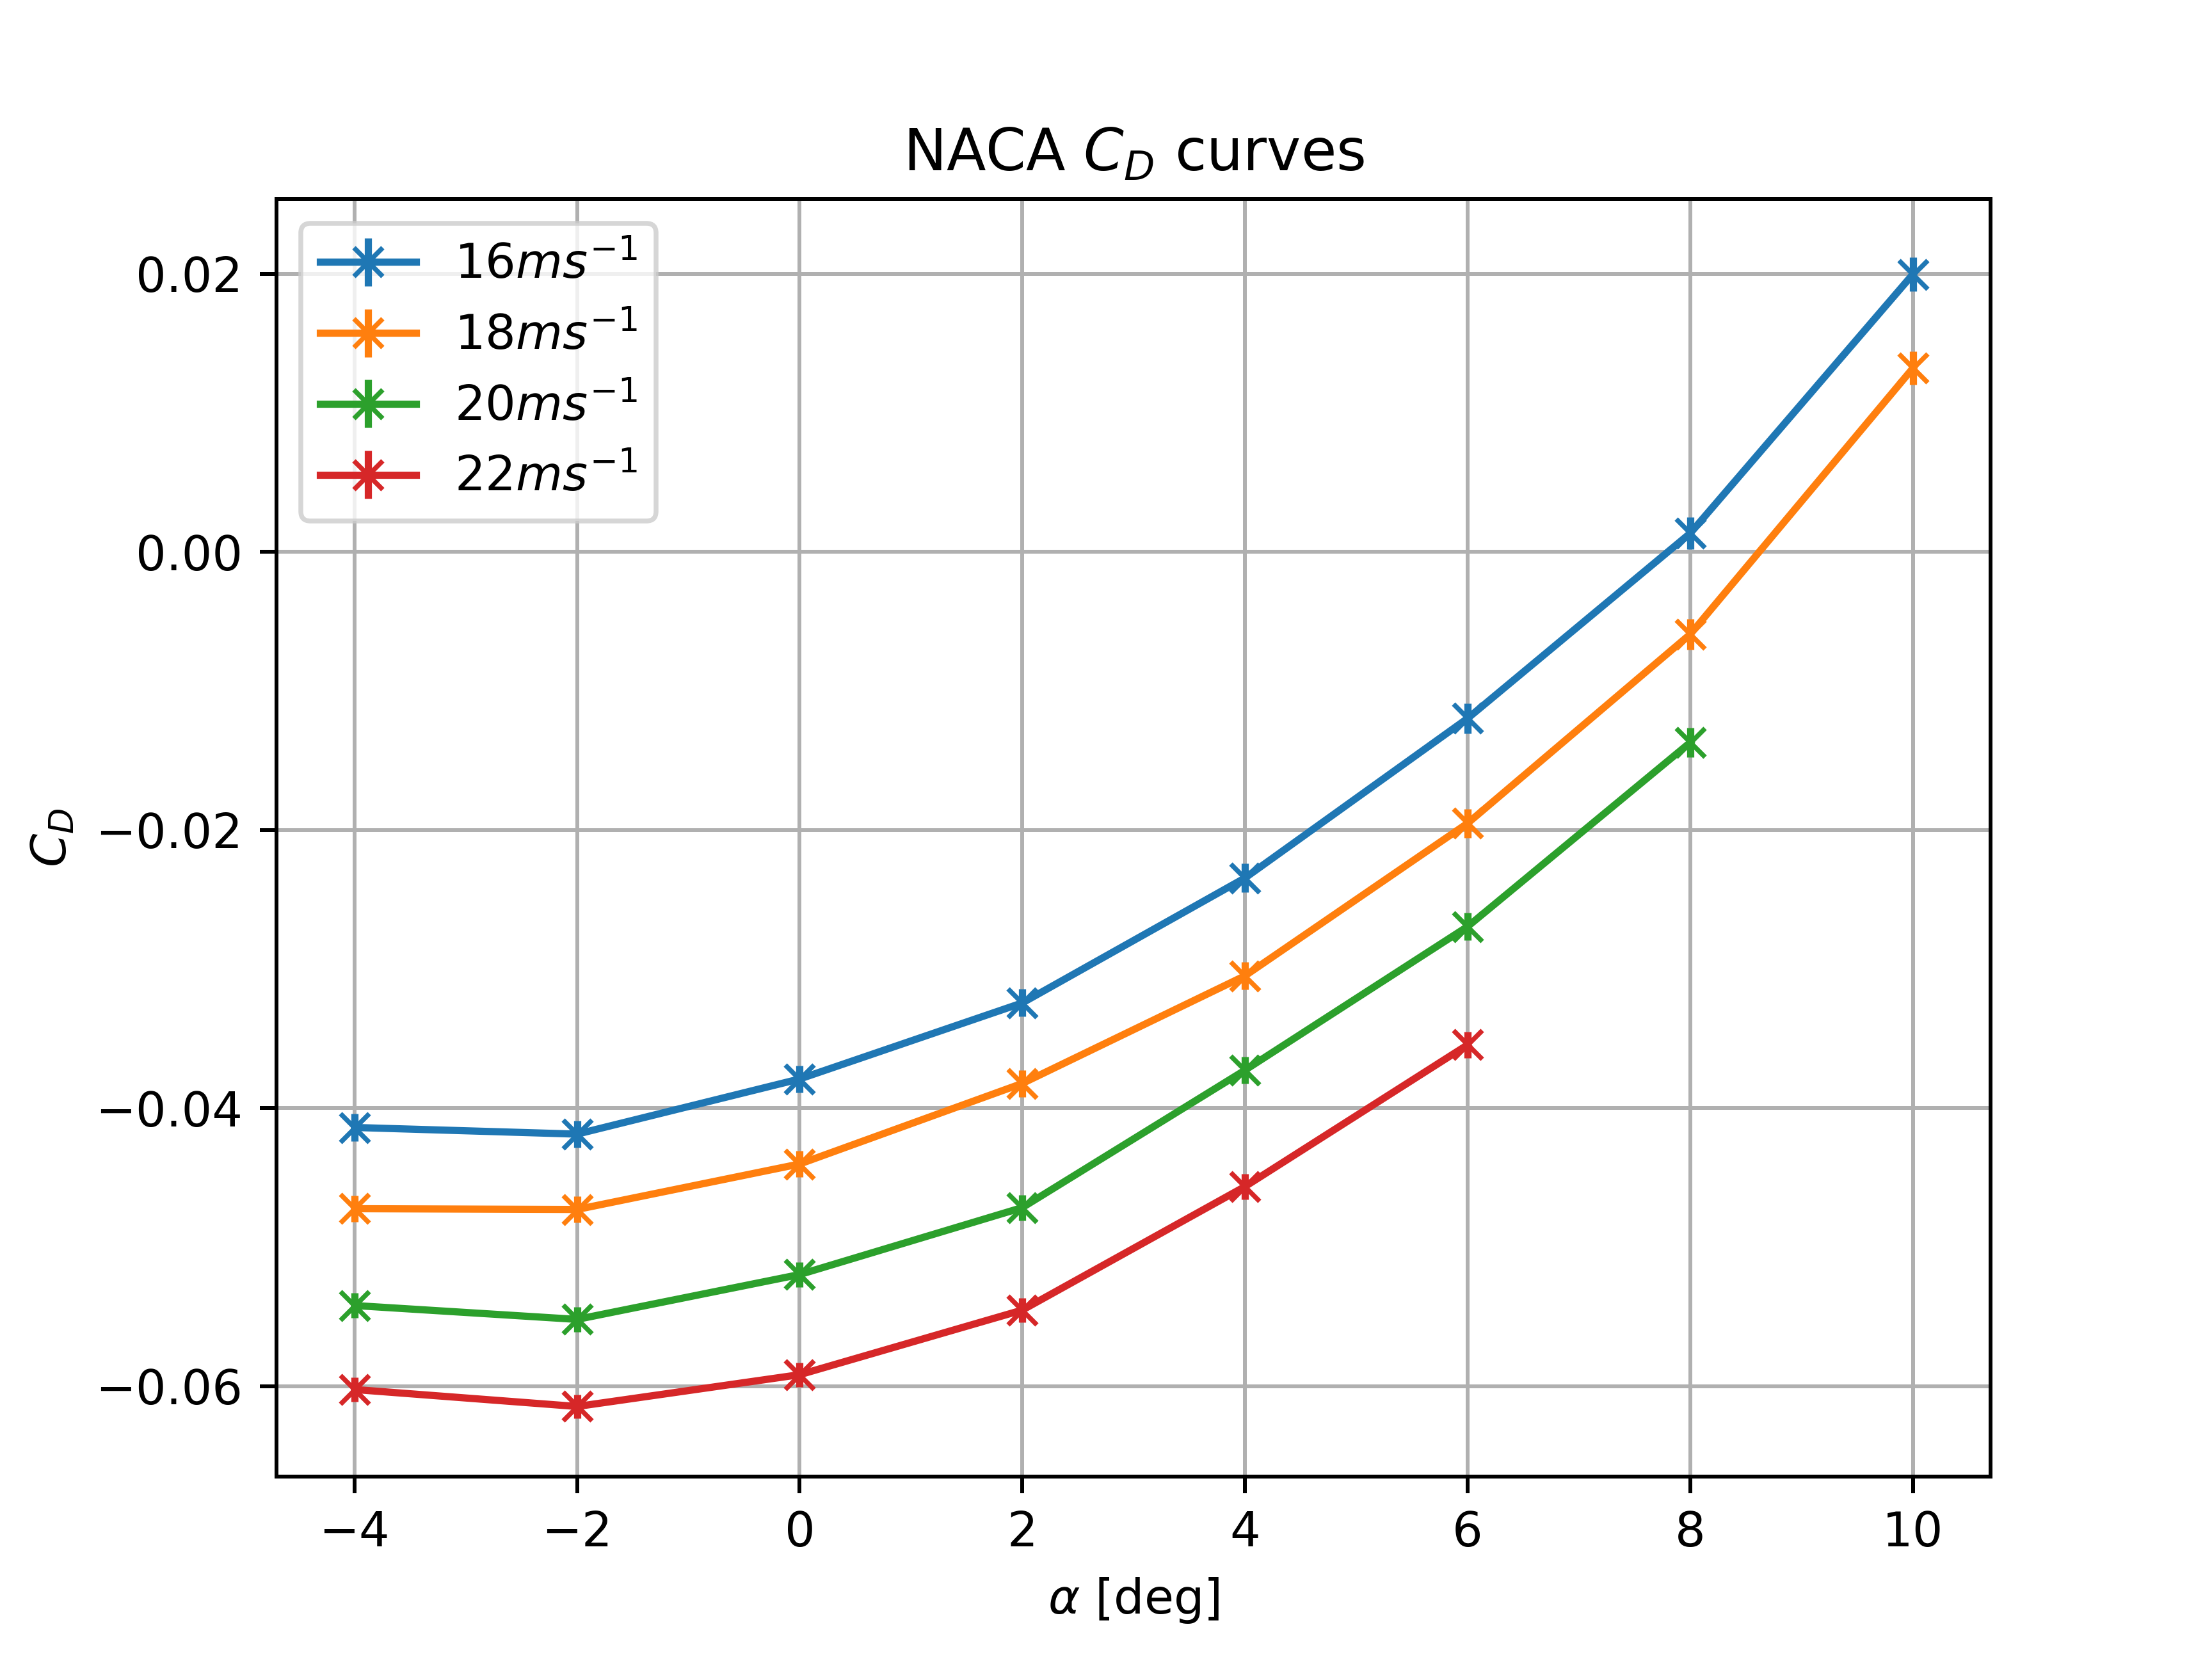
\includegraphics[width=\textwidth]{naca-drag-coefficient}
        \caption{NACA drag coefficient}
        \label{fig:wind-tunnel-results:naca-drag-coefficient}
    \end{subfigure}
    \hfill
    \begin{subfigure}[b]{0.49\columnwidth}
        \centering
        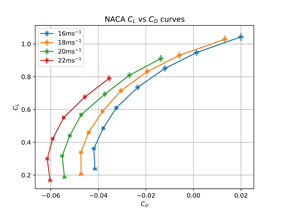
\includegraphics[width=\textwidth]{cl-against-cd}
        \caption{$C_L$ against $C_D$}
        \label{fig:wind-tunnel-results:cl-against-cd}
    \end{subfigure}

    \begin{subfigure}[b]{0.49\columnwidth}
        \centering
        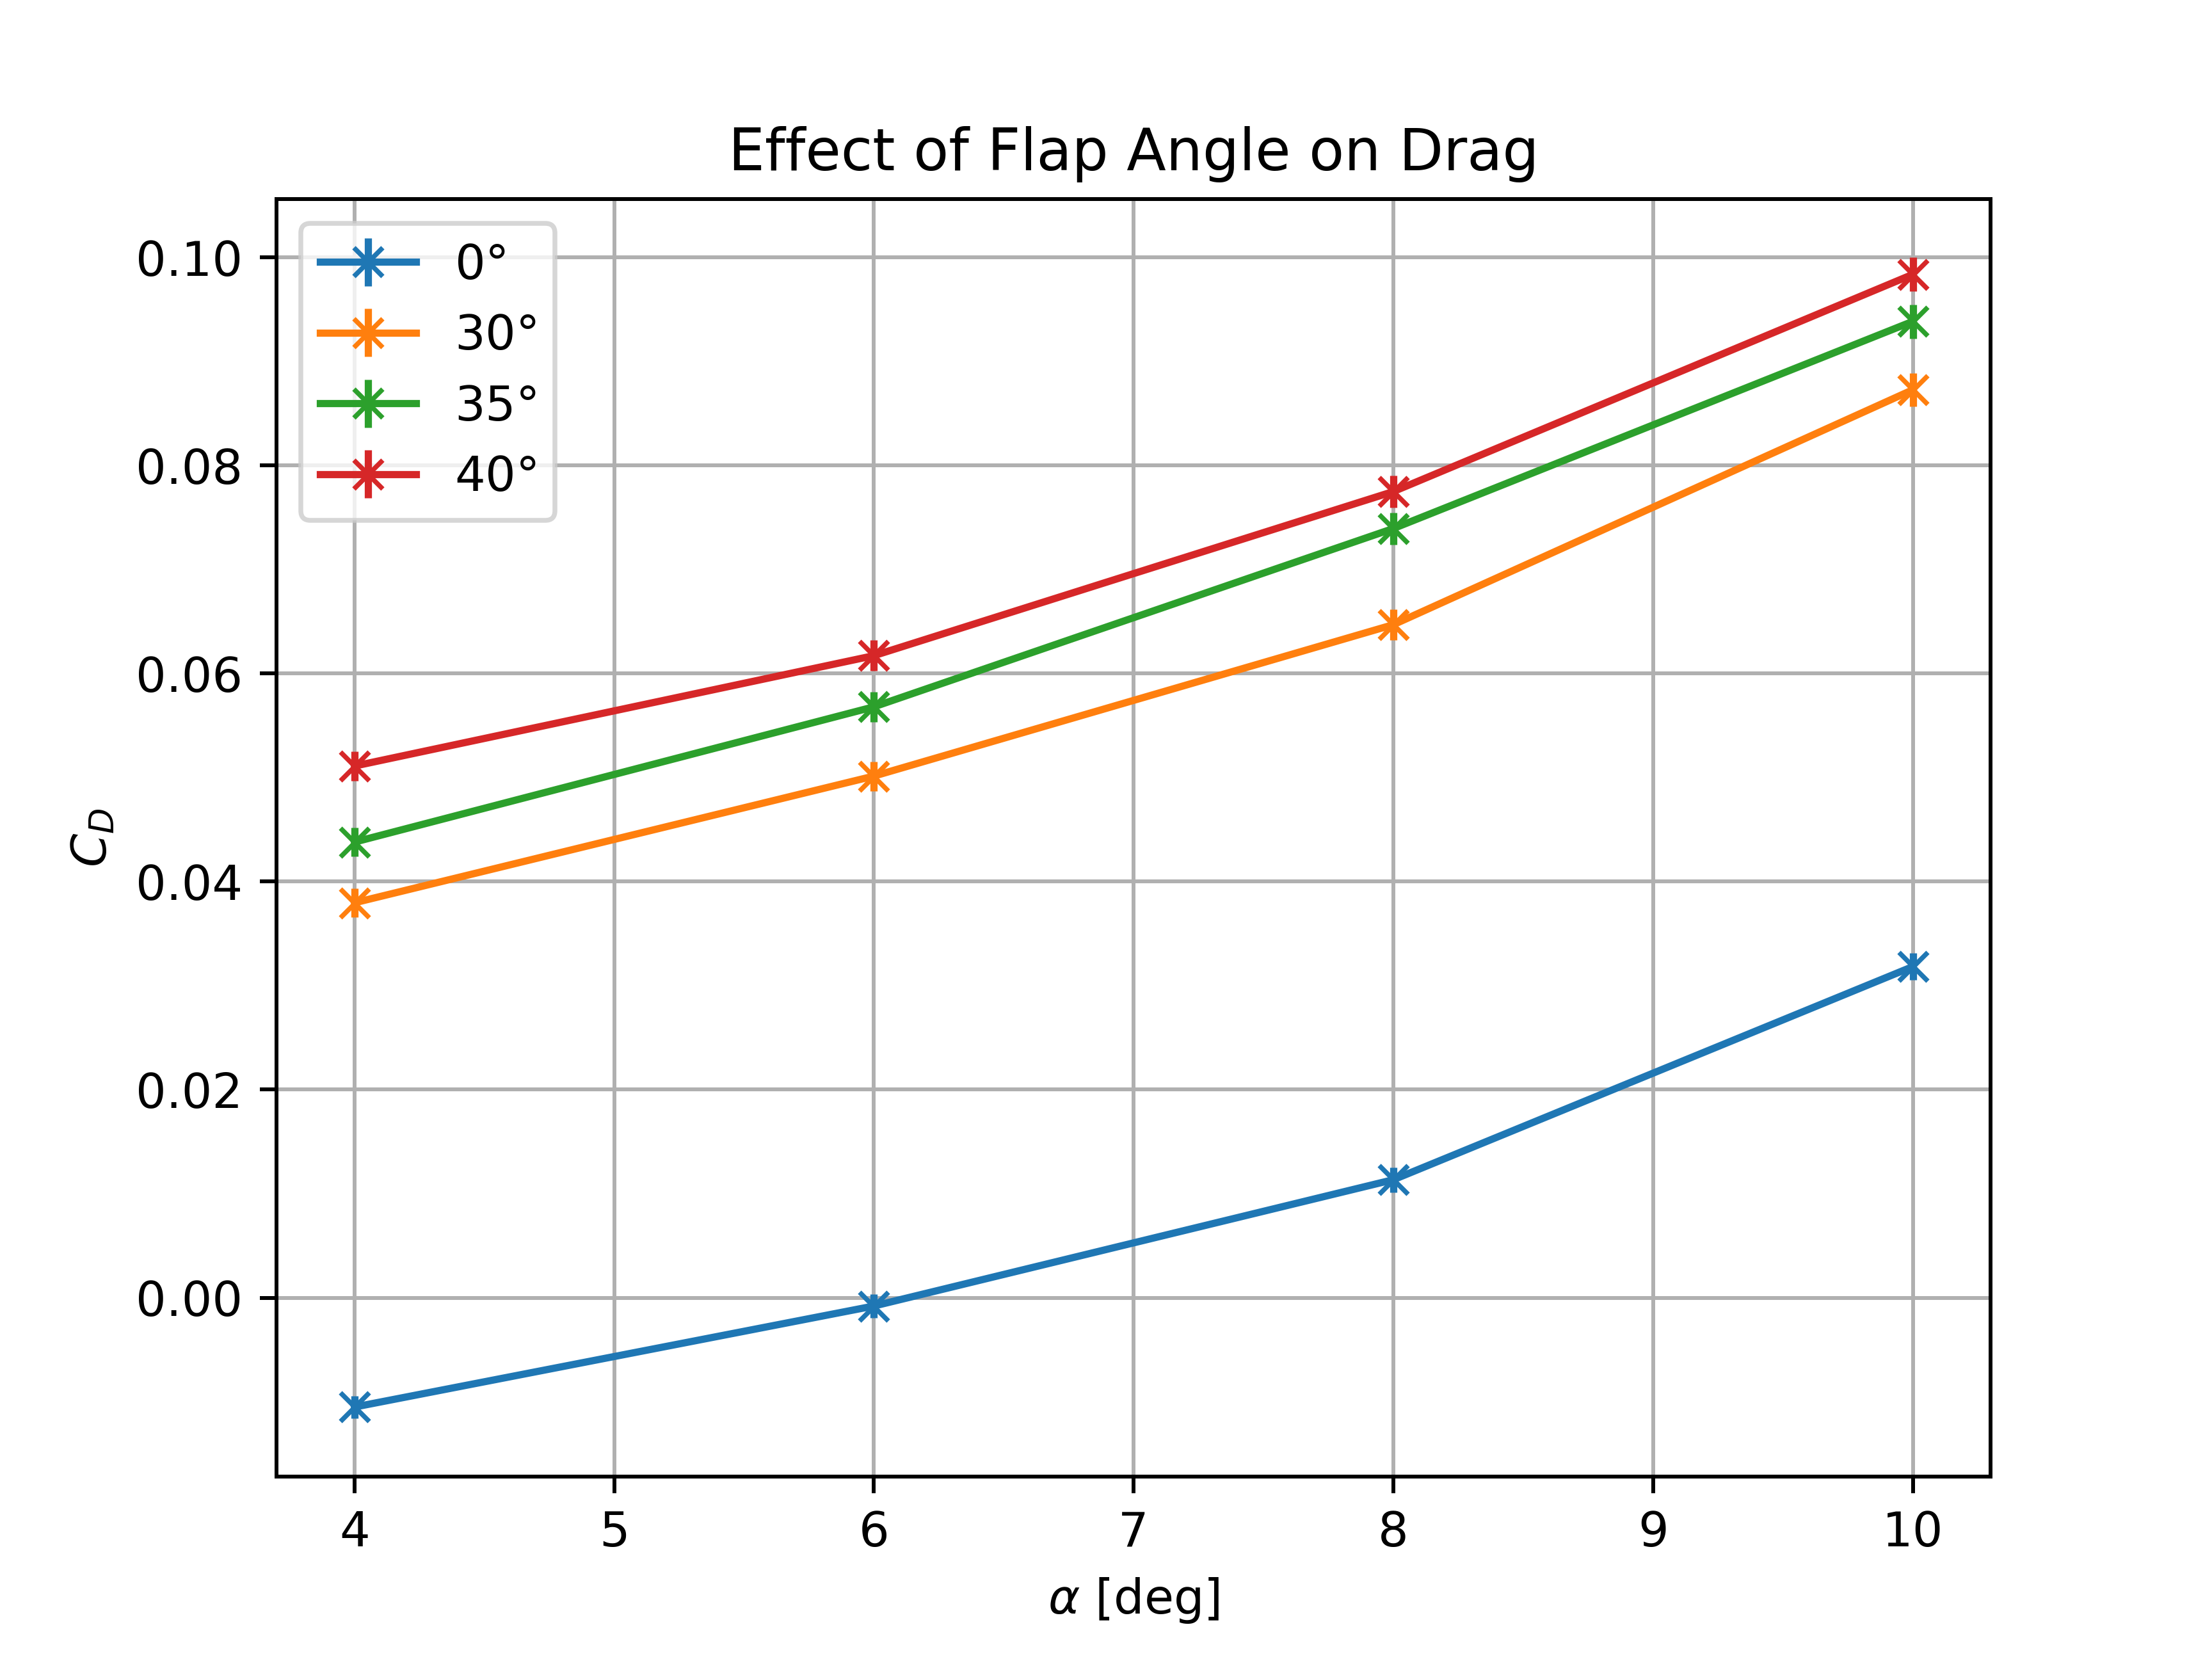
\includegraphics[width=\textwidth]{flap-drag-comparison}
        \caption{Flap drag comparison}
        \label{fig:wind-tunnel-results:flap-drag-comparison}
    \end{subfigure}
    \hfill
    \begin{subfigure}[b]{0.49\columnwidth}
        \centering
        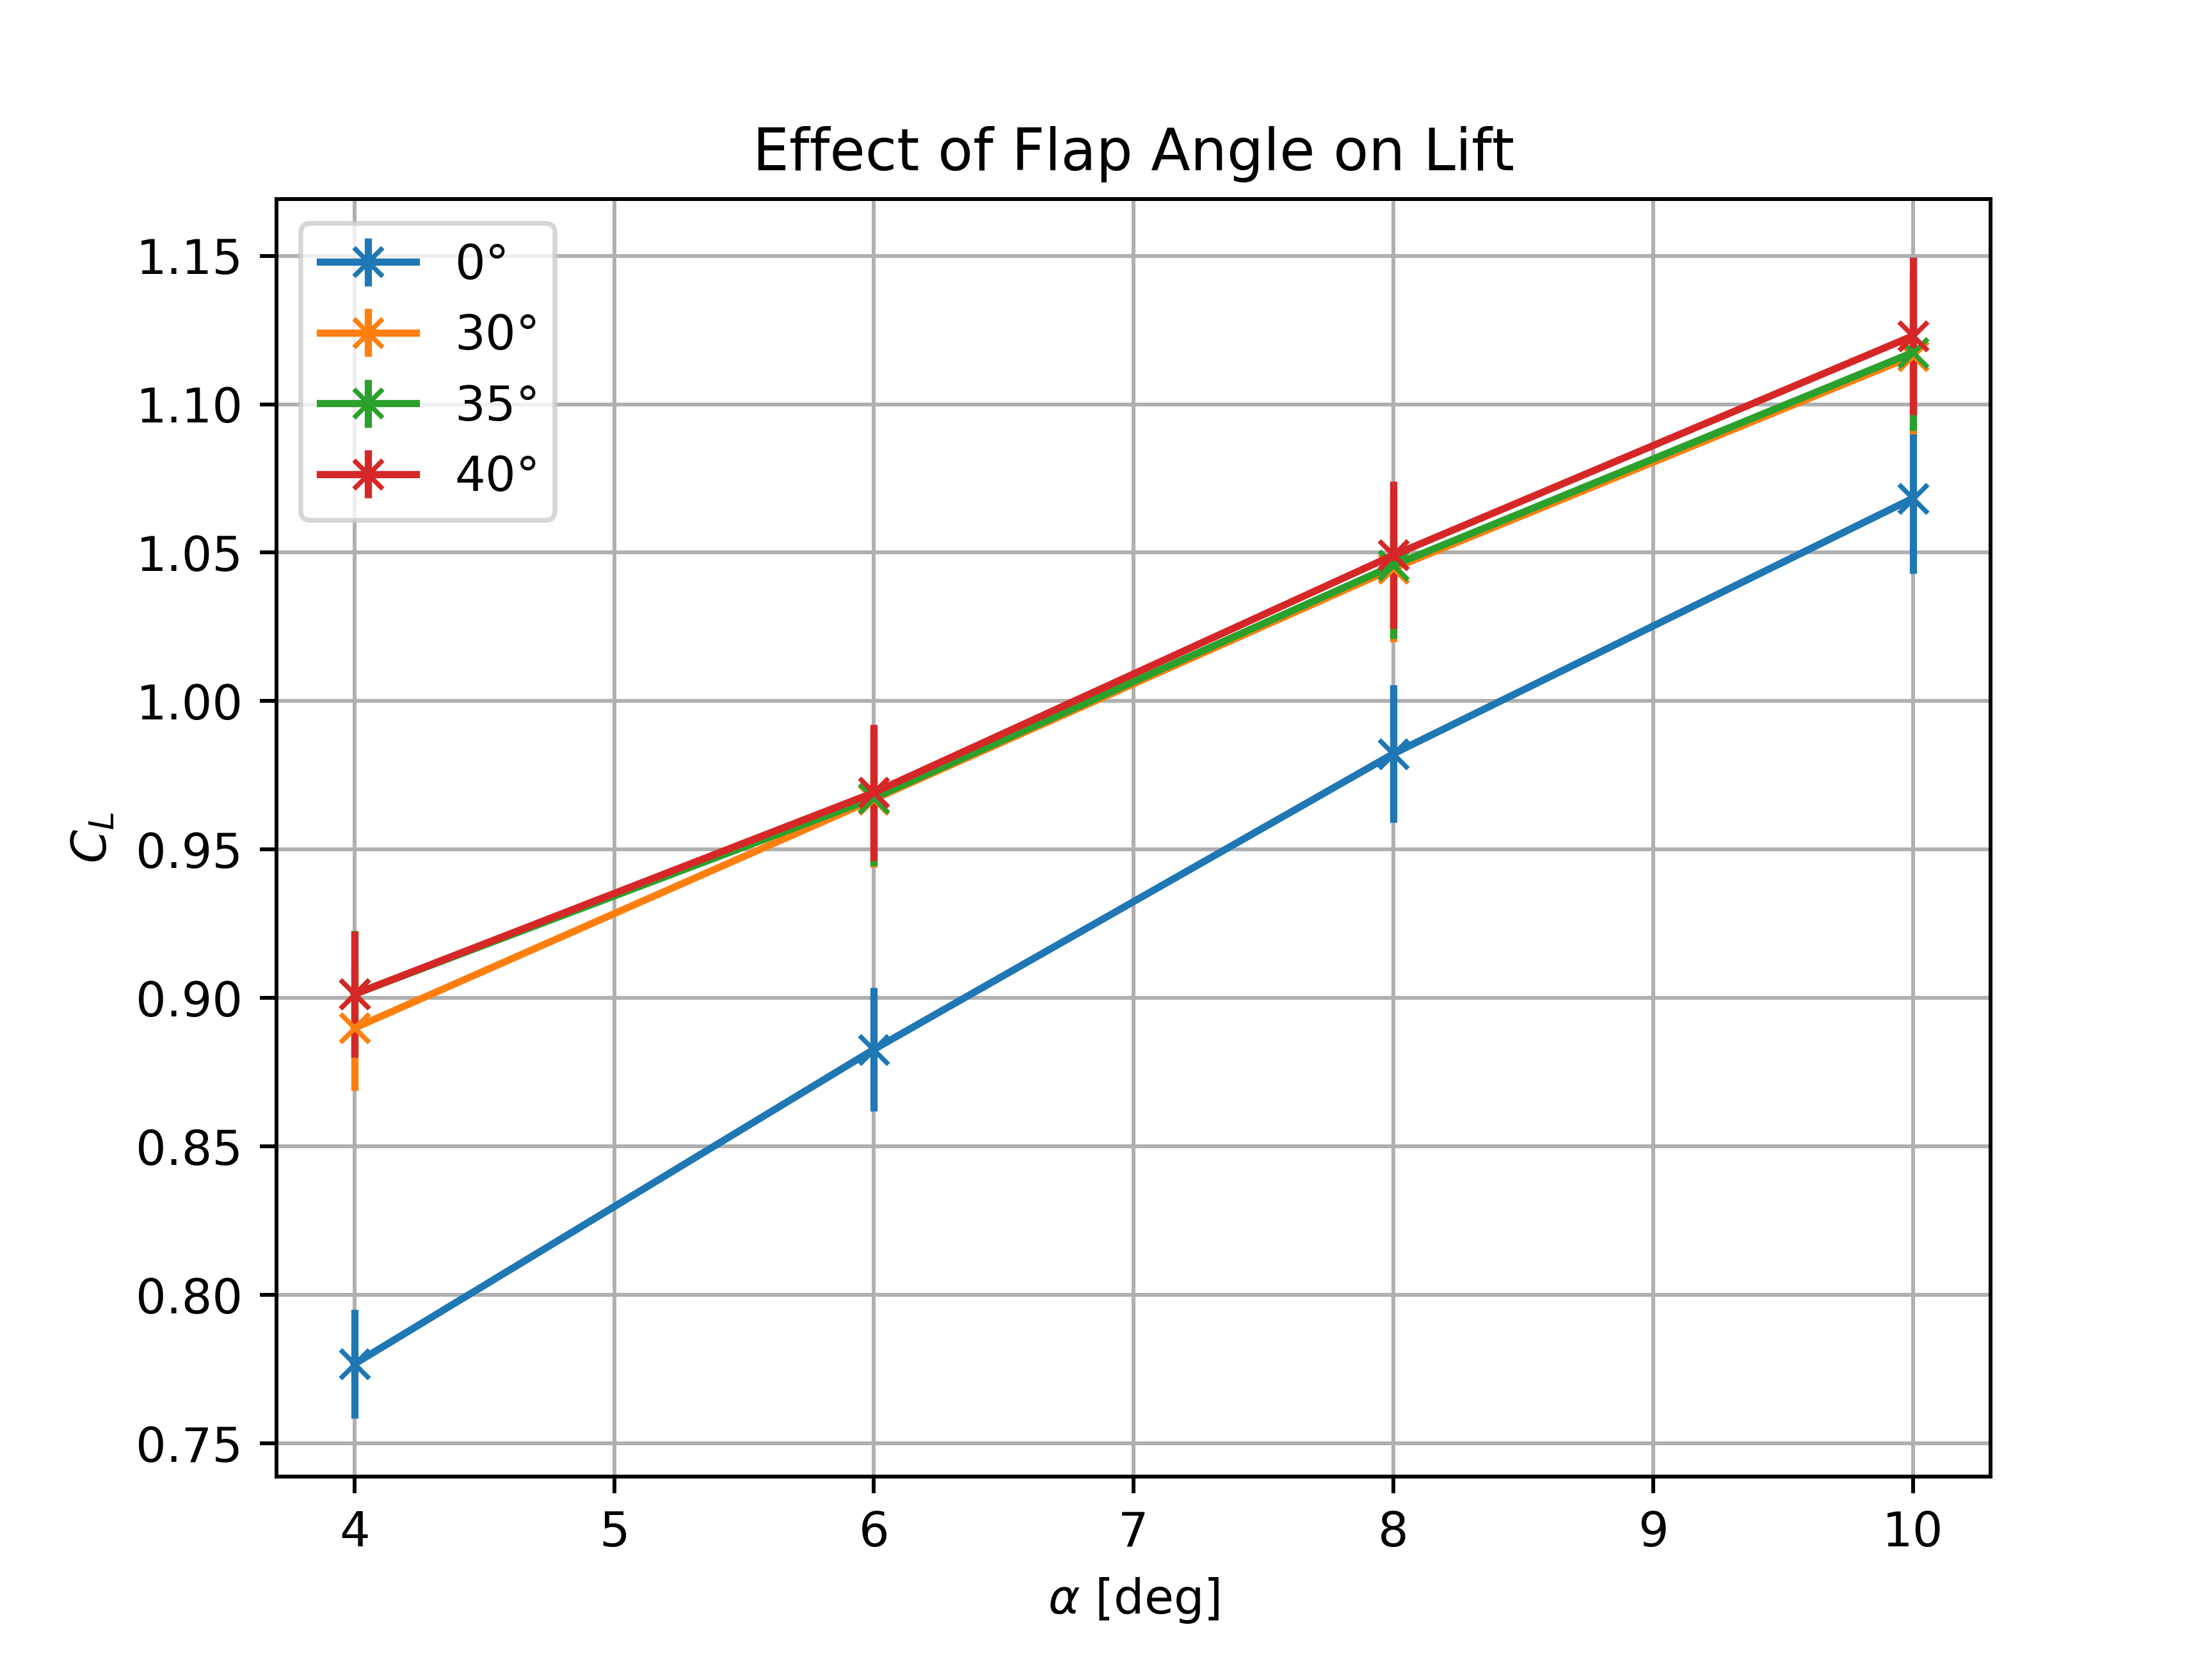
\includegraphics[width=\textwidth]{flap-lift-comparison}
        \caption{Flap lift comparison}
        \label{fig:wind-tunnel-results:flap-lift-comparison}
    \end{subfigure}

    \begin{subfigure}[b]{0.49\columnwidth}
        \centering
        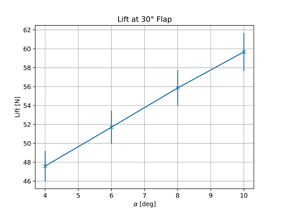
\includegraphics[width=\textwidth]{30-degree-flap-lift}
        \caption{30$^o$ flap lift}
        \label{fig:wind-tunnel-results:30-degree-flap-lift}
    \end{subfigure}
    \hfill
    \begin{subfigure}[b]{0.49\columnwidth}
        \centering
        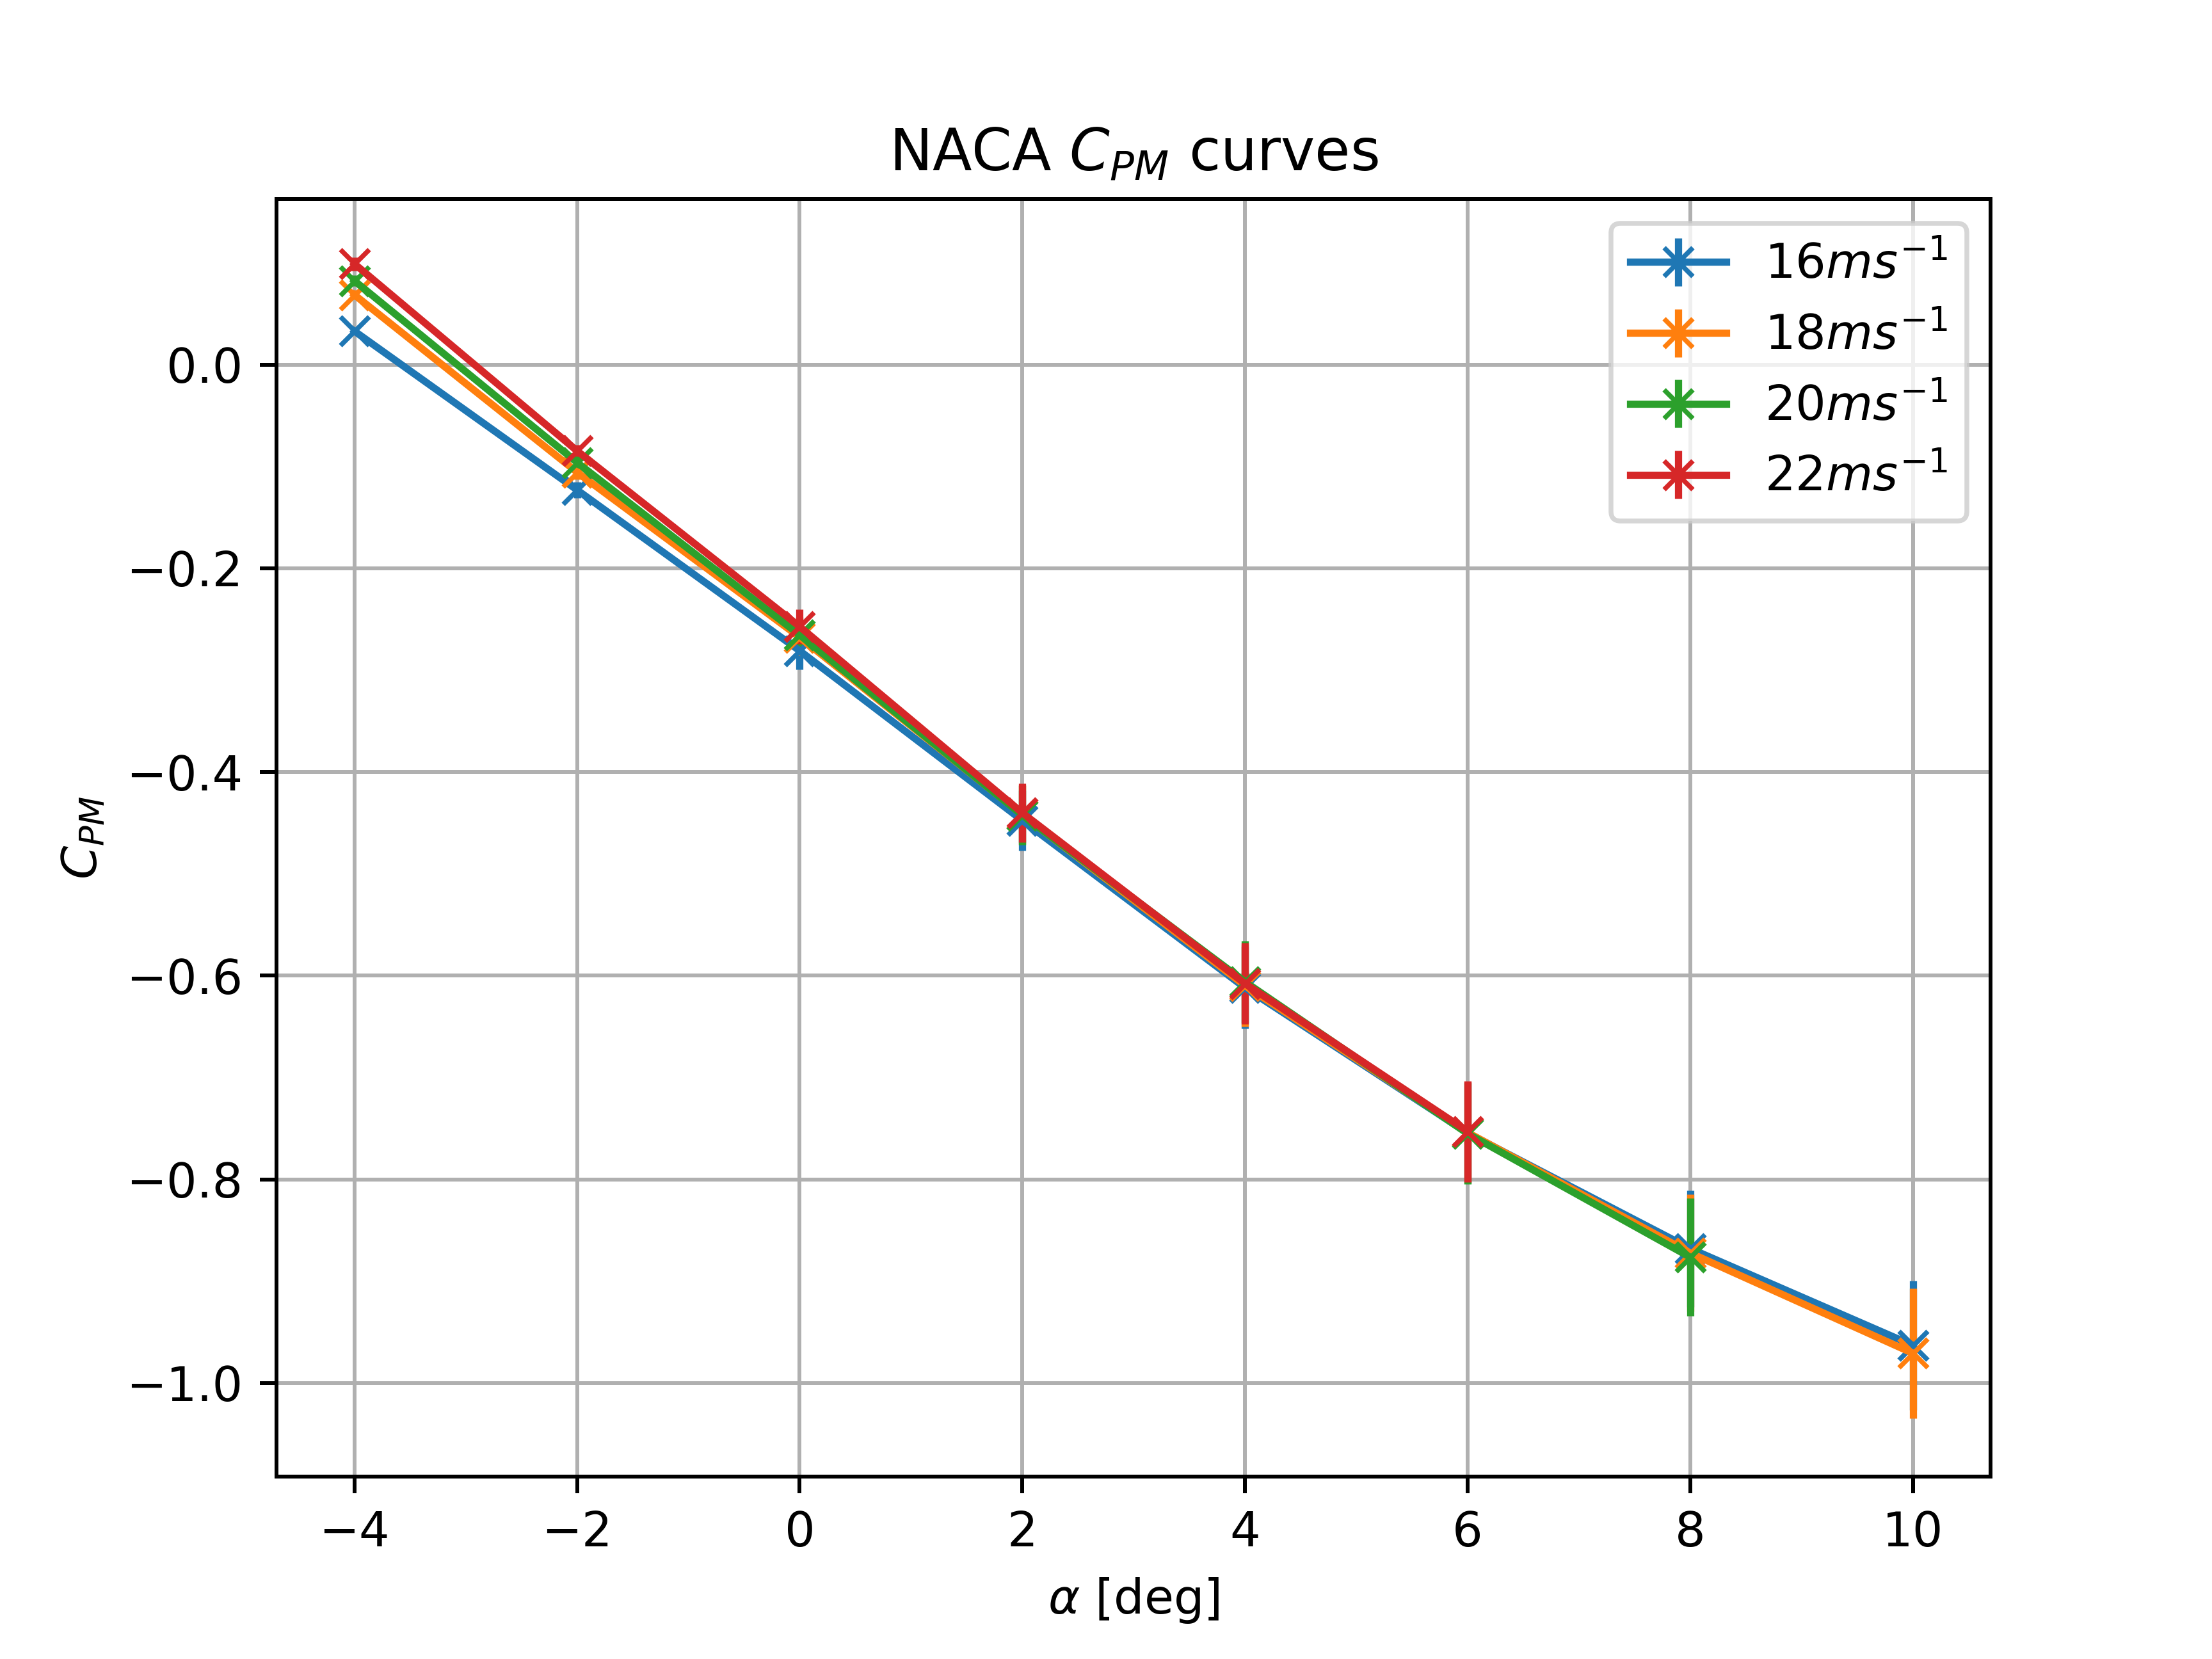
\includegraphics[width=\textwidth]{moment-coefficients}
        \caption{Moment coefficients}
        \label{fig:wind-tunnel-results:moment-coefficients}
    \end{subfigure}

    \caption{graphical results of the analysis of data gathered during the wind tunnel test.}
    \label{fig:wind-tunnel-results}
\end{figure}

The results from the wind tunnel test required considerable post processing before analysis could be carried out, but once this was complete the graphs could be made, and the results could be easily analysed.
There was a significant problem when the correction for the drag of the mounting structure, used to hold the model in the wind tunnel, was implemented because it caused some of the drag results to be negative.
This is a significant problem and means that the drag data is unreliable, however the trends seen in the results can still be useful.
The drag data will now rely on CFD and additional wind tunnel tests for clarification.
Figure 1 a) shows the results from the initial test carried out, where the setting angle of the two wings were found by increasing the angle of the wing against the fuselage until the lift exceeded the target weight of 70N at the target cruise speed of 20m/s.
This graph shows that the NACA 6412 exceeded this lift at 1, and so was set at 2 for the rest of the test to give a margin as the final wing is expected to produce slightly less lift due to the attachment of the propulsion units.
The Clark Y exceeded the required lift at around 3 and so was set at 4 for the same reason. 

Figure 1 b) and c) show the comparison between the NACA 6412 and Clark Y wings through a full sweep of angle of attack.
At this point the wing were set at their specified angles, and so the whole model was moved through the range of angles of attack to give the data.
It can be seen that the two wings produce very similar $C_L$ values, this is expected thanks to setting the wings at their respective angles, however the Clark Y aerofoil stalls before the NACA 6412, thus giving a lower maximum lift, and this is one of the reasons the NACA 6412 was chosen as the aerofoil for the final UAV instead of the Clark Y.
It can also be seen that the Clark Y has a higher $C_D$ at all angles of attack, and so is less efficient than the NACA 6412, and so the NACA 6412 was chosen. 

Figure 1 d) e) and f) show the plots for the wind tunnel model equipped with the NACA 6412 at a range of airspeeds showing the performance throughout the target flight envelope of the UAV.
Figure 1 d) shows that the $C_L$ remains almost constant as the airspeed changes, as expected as there are no compressibility effects as these speeds.
Figure 1 e) shows that the $C_D$ reduces with the increase in airspeed, this is due to the reduction of lift induced drag at higher speeds.
Figure 1 f) shows that therefore the highest aerodynamic efficiency is found at the highest tested speed of 22m/s, and although this speed is above the targeted cruise speed of the UAV, it shows that for maximum range, the UAV should be flown as fast as possible. 

Figure 1 g) and h) show the results of the flap test that was performed with the NACA 6412 wing.
Figure 1 g) shows the increase in $C_D$ that comes with each increase of the flap angle, and Figure 1 h) shows that the $C_L$ increases significantly with the flaps activated, but that the variation of the flap angle has little to no effect on the increase in $C_L$.
This suggests that the flaps are stalling at 30, and so the flap angle to be used in the final model will be 30.
Figure 1 i) shows that the lift increase was not enough to provide the required lift at the target take-off/landing speed of 12m/s, with the maximum lift produced being just under 60N at 10.
The wing has not stalled at this point and so there is possibility for the wing to produce more lift at a higher angle of attack, however this could not be tested as 10 was the highest angle that could be reached.
Even so, it is clear that the design of the flaps needs to be modified to improve their effectiveness, and also the area of the wing used for the flaps could be increased in order to maximise their effectiveness. 

The wind tunnel test also provided data for the pitching moment about the aerodynamic centre of the wing, as shown in Figure 1 j), which gives an insight into the aerodynamic stability of the model and the pitching moment developed by the wing.
The data shows that the coefficient of pitching moment is independent of airspeed, and that its negative at 0 angle of attack, which is not ideal as it means that the aircraft would want to pitch down and so the pilot would need to trim the model, or use constant elevator in order to fly level.
However the negative gradient of the line on the plot is good as this means that the aircraft is aerodynamically stable in pitch, so any pitching up of the aircraft would produce an increase in the pitching down moment and the aircraft would automatically stabilise.
Also, with an adjustment to the tail-plane, the magnitude of the pitching moment could be made zero at 0 angle of attack by producing a counteracting moment with an angled tail-plane, and then the pilot would not need to trim the aircraft by such a significant magnitude. 

The uncertainty of the results has been calculated for all results and is shown as vertical bars for every point on the plots in Figure 1.
The uncertainties were calculated using the know accuracies of the recorded results, as well as repeats performed during the testing.
The maximum number of repeats for one test was only 2, and so the sample size is not significant, but the uncertainties are still reasonably small even with a 95.45\% confidence.
These uncertainties were then converted to percentages and applied to all results of that type, with an example table for the uncertainty of $C_L$ shown in Table 1, and the others provided in the appendix. 

% TODO: insert table from &REF2
% TODO: units
% TODO: define uncertainty and variance outside table
% TODO: reduce width slightly
\importtable{|
    >{\raggedright\arraybackslash}m{0.16\columnwidth}
    >{\raggedleft\arraybackslash}m{0.16\columnwidth}
    >{\raggedleft\arraybackslash}m{0.17\columnwidth}
    >{\raggedleft\arraybackslash}m{0.17\columnwidth}
    >{\raggedleft\arraybackslash}m{0.17\columnwidth} |
}{
    \hline
    Measured variable & $L$ & $q$ & $S$ & Rep. $C_L$ \\
    \hline
    Typical value & 77.04 & 249.55 & 0.6 & 0.01715 \\
    Accuracy & 0.07704 & 0.349 & 0.0012 & 0.01213 \\
    PDF & rect. & rect. & rect. & norm. \\
    PDF factor & 1.7321 & 1.7321 & 1.7321 & 1 \\
    $k$ factor & 1 & 1 & 1 & 1 \\
    SC value & 0.006679 & -0.00206 & -0.85754 & 1 \\
    Uncertainty & 0.000297 & -0.000416 & -0.000594 & 0.012128 \\
    Variance & $9\times10^{-8}$ & $1.7\times10^{-7}$ & $3.5\times10^{-7}$ & $1.471\times10^{-4}$ \\
    \hline
}{uncertainty calculations for $C_L$.}{cl-uncertainty}

\importtable{| l r |}{
    \hline
    Combined standard uncertainty & 0.01215 \\
    $C_L$ mean & 0.5145 \\
    Percentage uncertainty & 2.36 \\
    \hline
}{uncertainty summary for $C_L$.}{uncertainty-summary}

Unfortunately, the scope of the work required to design a fully functional tailplane with control surfaces had not been realised at this point, and the design was far too simple, with no mounting angle or control surfaces.
The tail was also undersized based on observation by our project supervisors.
Because of this, little work went into analysing the results from this test in terms of the tailplane, and work on the next version essentially started from scratch. 

\subsection{Motor and propellor test} \label{sec:design-process:interim-design-review:motor-and-propellor-test}

\subsubsection{Overview} \label{sec:design-process:interim-design-review:motor-and-propellor-test:overview}

\importimage{motor-bracket}{the motor bracket attached to the rear of the motor.}{Motor bracket}{0.5}
\importimage{motor-test}{the motor in the wind tunnel.}{Motor test}{0.5}

Once the motor and propeller selection had been completed based on wind tunnel results and propeller performance analysis, we ordered one of the wing motors with its tractor configuration propeller in order to test them together.
This test was to be performed in a small wind tunnel so as to give data for the motor in flight as well as a static thrust test.
The motor mount is a load cell located at the centre of the wind tunnel section, as shown in Figure 1 b), and to attach the motor a bracket is required.
The main part of this bracket had already been made for the testing of a different motor by the university, and so only a small plate was required to mount our motor to the existing setup.
This mount was made from aluminium sheet to fit to the back of the motor and mount onto the load cell, and is shown in Figure 1 a).
It required some precision marking and drilling for the outer holes as there were tight tolerances on the bracket it was to attach to, while the motor holes could be slightly less precise due to the countersunk bolts holding it in place.
A central clearance hole was required to allow the motor shaft to pass through, into the void created by the existing bracket in order to avoid the motor shaft hitting against the load cell.
The tests carried out were at wind speeds of 0m/s, 10m/s, and 15m/s, and at each wind speed the voltage was held at around 14.9V representing a partially drained battery, and the current was varied from 0 to 22A, giving a range of RPM at which we collected the thrust and torque data up to a max power of 330W.
The RPM was measured from the input to the motor, rather than directly from the blades, because the blades of the propeller were too short to reach in front of the laser.
However, this RPM data is accurate enough for this experiment.
The load cell used to mount the motor formed a blockage in the wake of the propeller, and so this will have affected the results, however the effect of this was reduced as much as possible by manufacturing the bracket to be as small as possible.
Also, the motor when attached to the model will have the blockage of the wing and the power unit housing behind it, so this effect is a good representation of the motor in flight.
Additionally, in order to maximise the performance of the propeller, it was sanded before the test to remove any manufacturing defects and to ensure a smooth surface for the airflow.
The propeller was balanced by the manufacturer, and during the test showed no significant signs of imbalance, with the output data remaining smooth throughout the test showing no signs of large vibrations. 

\subsubsection{Results and analysis} \label{sec:design-process:interim-design-review:motor-and-propellor-test:results-and-analysis}

\importimage{manufacturer-comparison}{comparison between the power data quoted by the manufacturer and the data collected in the wind tunnel.}{Manufacturer comparison}{0.8}

Figure 1 shows that the data provided by the propeller supplier and the data from the test performed match up very well for the power output from the propeller at a given RPM, this shows that the data provided is accurate and can be used as a good estimate of the power provided by the other propellers intended for use on the UAV, the pusher version of the propeller tested and both fuselage propellers. 

\importimage{thrust-data}{thrust data collected at the three airspeeds tested.}{Thrust data}{0.8}

Figure 2 shows again the similarities between the data given by the propeller supplier for the static case and the test data, but more importantly this graph shows the drop off of thrust with an increase in airspeed.
This can be used to estimate the thrust developed by the propulsion unit at cruise, and so find if the propeller is suitable for use.

\importimage{maximum-thrust}{maximum thrust at the airspeeds tested, with an extrapolation to the intended cruise speed of 20 m.s-1}{Maximum thrust}{0.8}

Figure 3 shows the extrapolation of the thrust of the propulsion unit at different airspeeds up to the intended cruise speed of 20m/s.
This predicts that the thrust in cruise would be 6.5N, therefore 13N for the total thrust of the UAV.
From CFD drag results giving 10N at 20m/s, this would be sufficient to cruise at 77\% throttle, saving battery and giving a longer flight time than if cruise had required full throttle. 

\importimage{efficiency-data}{efficiency data collected at the three different airspeeds tested}{Efficiency data}{0.8}

Figure 4 shows the efficiency curves for the power unit at different airspeeds, and also the data provided by the supplier for the propeller at static conditions.
From this data it is clear to see a significant difference between the data provided by the propeller manufacturer and the data recorded, which is surprising given that the power produced by the propeller is so similar to the manufacturer data.
This suggests that the difference is due to the motor used, and so suggests that the motor is providing a significant loss of power in the system.
If the difference is assumed to be entirely due to the motor, we can apply this back to the other airspeed cases to find the propeller efficiencies in these cases, this is assuming that the motor efficiency is not affected by the airspeed, only by its RPM.
This assumption would not be entirely accurate as the cooling would have an effect on performance, as well as the difference in drag on the rotating shell of the motor at different airspeeds.
However this effect is not important as the data needed is of the efficiency of the motor and propeller together, as is shown in the graph above, this data was then used to further update the constraint analysis and ensure that the power requirements were still met. 

\importimage{thrust-comparison}{comparison of thrust generated for a given input power at different airspeeds.}{Thrust comparison}{0.5}

Figure 5 shows how the effect of the motor efficiency lowers the thrust at a given input power.
This is due to the RPM of the propeller being lower for a given input power in the test than in the manufacturer data.
Also, this graph shows that the relationship between the thrust and the input power is tending towards an approximately liner relationship, and so the assumption that this is linear is a sensible one to make when updating battery life calculations.
Using this and the 77\% of max thrust required in cruise calculated earlier, we can assume that the power draw will be 77\% of the max, therefore giving an estimate battery life of just over 9 minutes if the power draw is constantly at this level, and so the flight time would be limited to 7 min for safety in order to ensure that the power does not cut off mid-flight. 

\section{Final design proposal} \label{sec:design-process:final-design-proposal}

\subsection{Wing} \label{sec:design-process:final-design-proposal:wing}

The wing assembly was designed to be unfasten from the fuselage assembly with ease.
Such decision was established so to reduce the encumbrance of the UAV during transportation.
The wing assembly is composed by two carbon spars placed respectively at quarter and half chord, and extending for the entire 2m wing span.
Each half of the wing presents three ribs, as shown in Fig.
0, obtained with the aid of additive manufacturing.
These cover multiple functions in the wing assembly as it will be later discussed.
The use of profiles carved out of blue Styrofoam (extruded polystyrene) provided a lightweight structure for the aerodynamic profiles such as flaps, aileron and wing itself.
A hollow profile also allowed the fitting of wires in the wing structure.
A central mounting plate provided the fitting points for the fastening of the wing assembly to the fuselage.

\subsubsection{Spars} \label{sec:design-process:final-design-proposal:wing:spars}

The two-spar structure utilized for the wind tunnel model’s wing exhibited small deflections in bending and twist when tested.
Therefore, this same configuration was maintained for the flight model.
Two carbon spars were used for the final design, thus reducing the weight although maintaining the same structural characteristics.
These have been sized for a case of a loading equal to 4g; at which the wing would present a deflection of 54mm at the wing tip as it can be seen in Fig. 1.
Both spars have a wall thickness of 2mm whereas their diameters differ.
The first one, position at quarter chord, has a diameter of 16mm; while the one positioned at half chord has a diameter of 14mm.

\importimage{fea-half-wingspan}{FEA of half wingspan subject to a distributed load of 138N/m.}{FEA of half wingspan}{0.5}

\subsubsection{Ribs} \label{sec:design-process:final-design-proposal:wing:ribs}

The attachment points for the power units are obtained through the use of 3D printed inserts imbedded in the wing structure.
These, as shown in Fig. 2, present the same airfoil section as the wing so to not disrupt the airflow.
Three inserts per half wingspan allow as many different possible propulsion positions: 20\% half-span, 40\% half-span and 100\% half-span (tip).
Thus allowing the assessment of the effects of the propulsion unit placed close to the fuselage structure (20\% half-span); at the optimal position shown in Propeller-wing interaction for minimum induced loss (Kroo, 1986) (40\% half-span) and wing tip (100\% half-span).
The design of this last is, although, different from the ‘mid-span’ elements.
For each of the mid-span inserts, the same motor unit can be mounted in four different configurations: top-tractor, bottom-tractor, top-pusher, bottom-pusher (Fig. 3).
While for the tip mounted element the available configurations are two: pusher, tractor (Fig. 4).
Adapters are adopted to blend the standardized connection surface of the motor housing with the wing’s surface.
Thus, reducing the aerodynamic footprint. 

% \importimage{mid-span-rib}{mid-span rib.}{Mid-span rib}{0.5}
% \importimage{tip-rib}{tip rib.}{Tip rib}{0.5}

\begin{figure}[H]
    \centering
    \begin{subfigure}[b]{0.49\columnwidth}
        \centering
        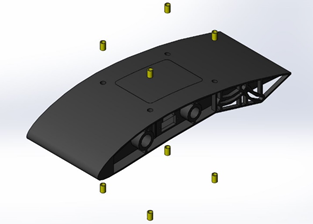
\includegraphics[width=\textwidth]{mid-span-rib}
        \caption{Mid-span}
        \label{fig:ribs:mid-span}
    \end{subfigure}
    \hfill
    \begin{subfigure}[b]{0.49\columnwidth}
        \centering
        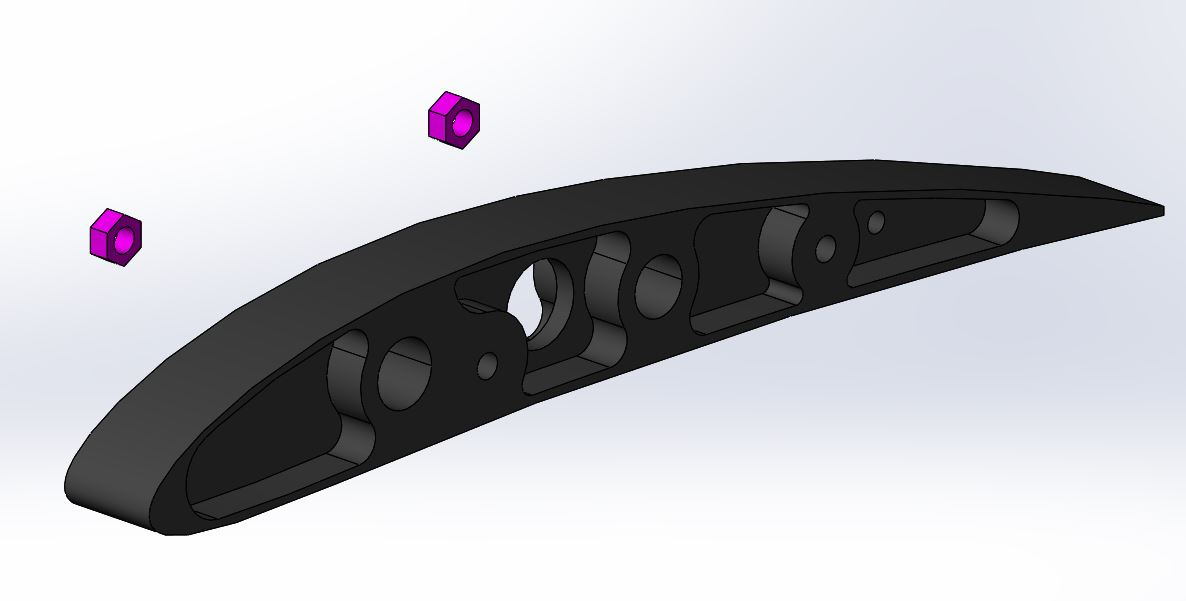
\includegraphics[width=\textwidth]{tip-rib}
        \caption{Tip}
        \label{fig:ribs:tip}
    \end{subfigure}
    
    \caption{CAD models of the wing ribs.}
    \label{fig:ribs}
\end{figure}

% \importimage{underwing-pusher}{underwing pusher configuration.}{Underwing pusher}{0.5}
% \importimage{underwing-tractor}{underwing tractor configuration.}{Underwing tractor}{0.5}
% \importimage{overwing-pusher}{overwing pusher configuration.}{Overwing pusher}{0.5}
% \importimage{overwing-tractor}{overwing tractor configuration.}{Overwing tractor}{0.5}
% \importimage{wingtip-pusher}{wingtip pusher configuration.}{Wingtip pusher}{0.5}
% \importimage{wingtip-tractor}{wingtip tractor configuration.}{Wingtip tractor}{0.5}

\begin{figure}[H]
    
    \centering
    \begin{subfigure}[b]{0.49\columnwidth}
        \centering
        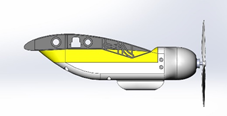
\includegraphics[width=\textwidth]{underwing-pusher}
        \caption{Underwing pusher}
        \label{fig:wing-mounting:underwing-puller}
    \end{subfigure}
    \hfill
    \begin{subfigure}[b]{0.49\columnwidth}
        \centering
        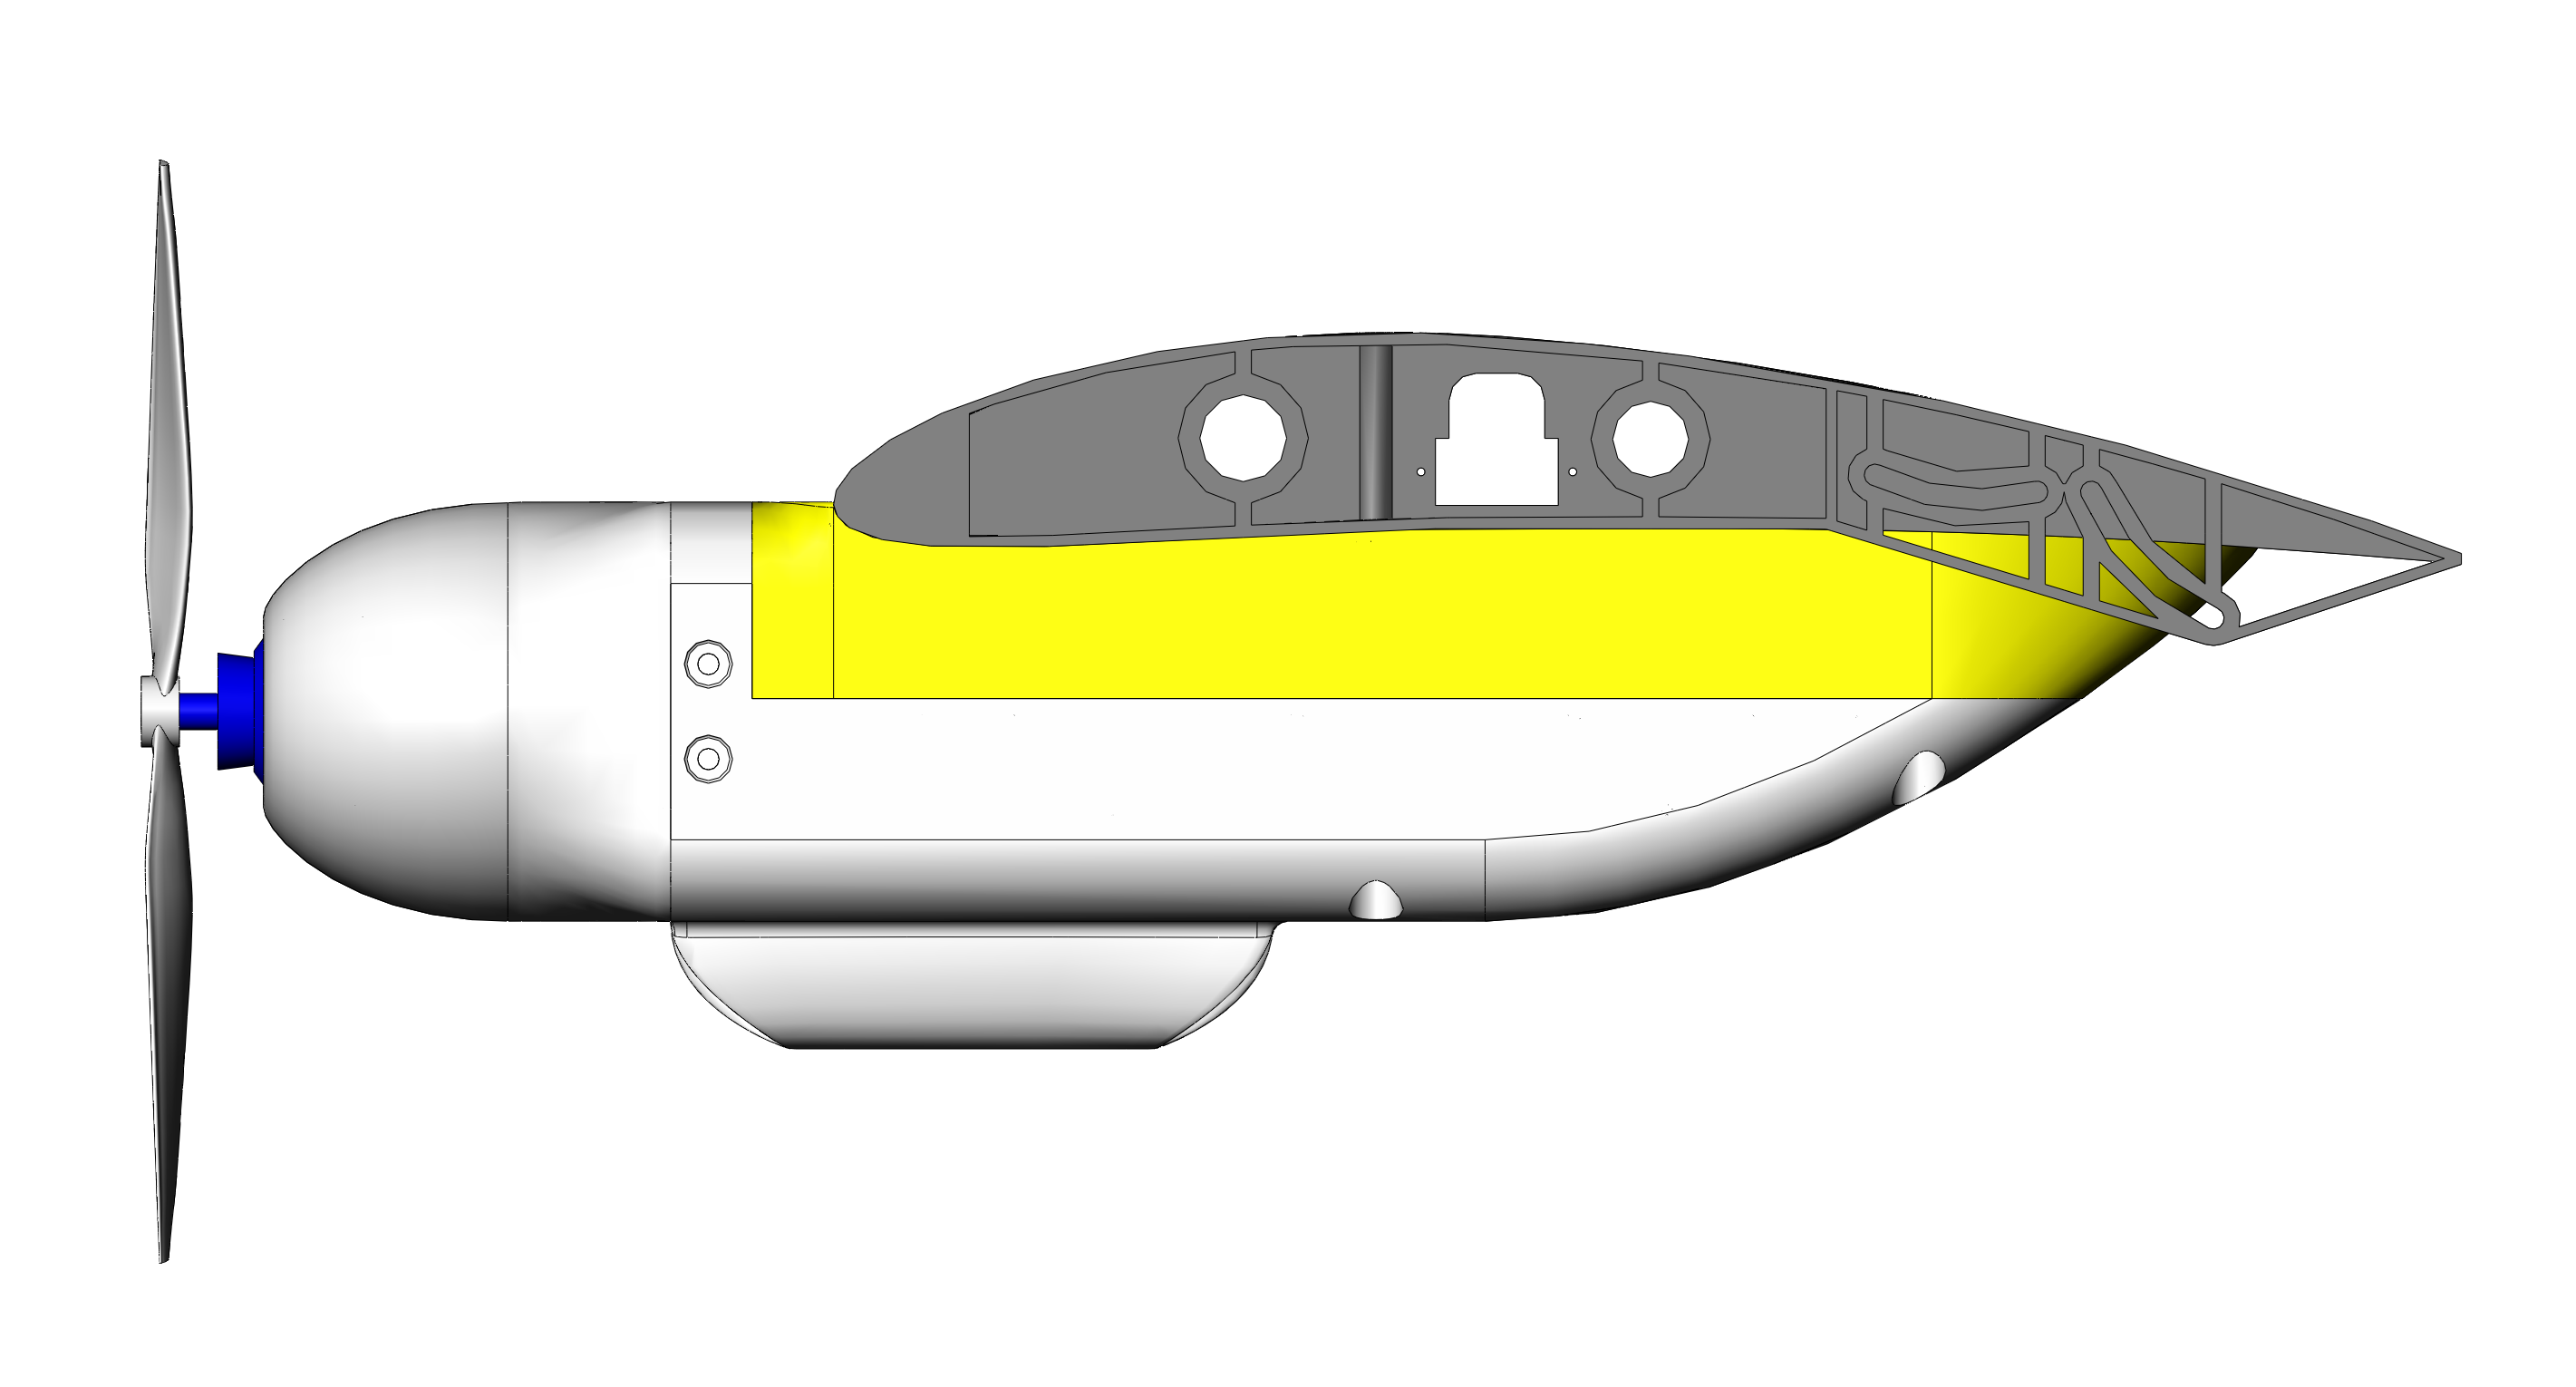
\includegraphics[width=\textwidth]{underwing-tractor}
        \caption{Underwing tractor}
        \label{fig:wing-mounting:underwing-tractor}
    \end{subfigure}
    
    \centering
    \begin{subfigure}[b]{0.49\columnwidth}
        \centering
        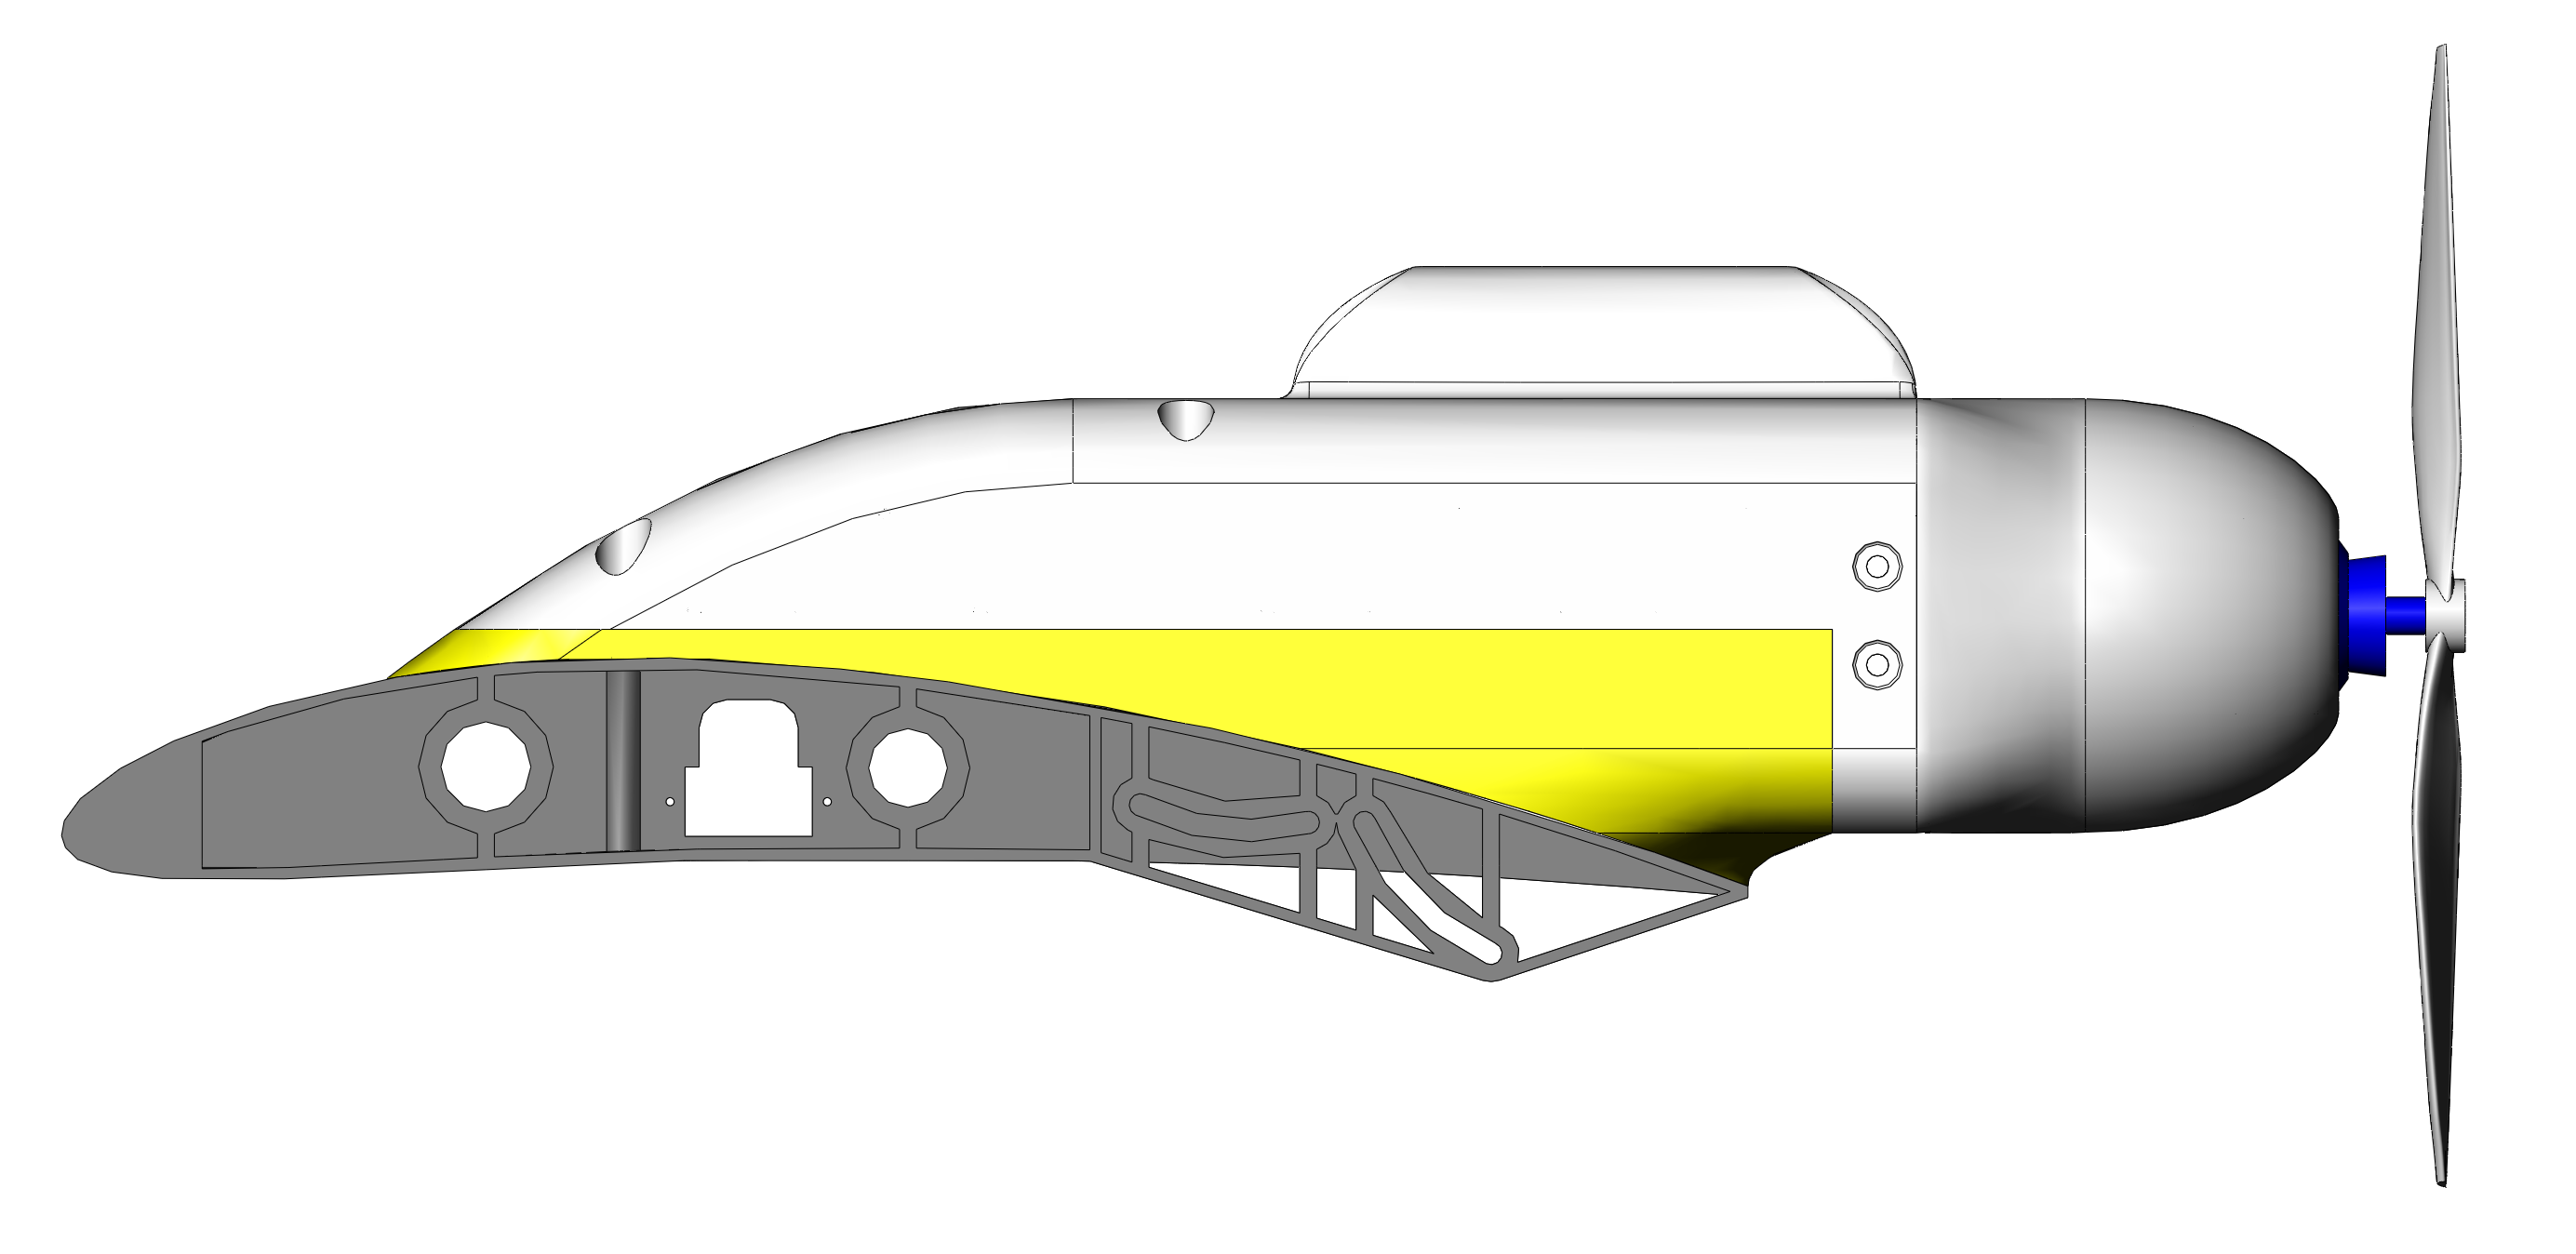
\includegraphics[width=\textwidth]{overwing-pusher}
        \caption{Overwing pusher}
        \label{fig:wing-mounting:overwing-pusher}
    \end{subfigure}
    \hfill
    \begin{subfigure}[b]{0.49\columnwidth}
        \centering
        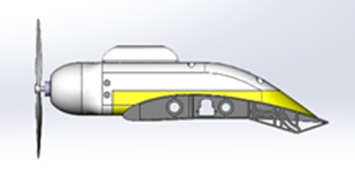
\includegraphics[width=\textwidth]{overwing-tractor}
        \caption{Overwing tractor}
        \label{fig:wing-mounting:overwing-tractor}
    \end{subfigure}
    
    \centering
    \begin{subfigure}[b]{0.49\columnwidth}
        \centering
        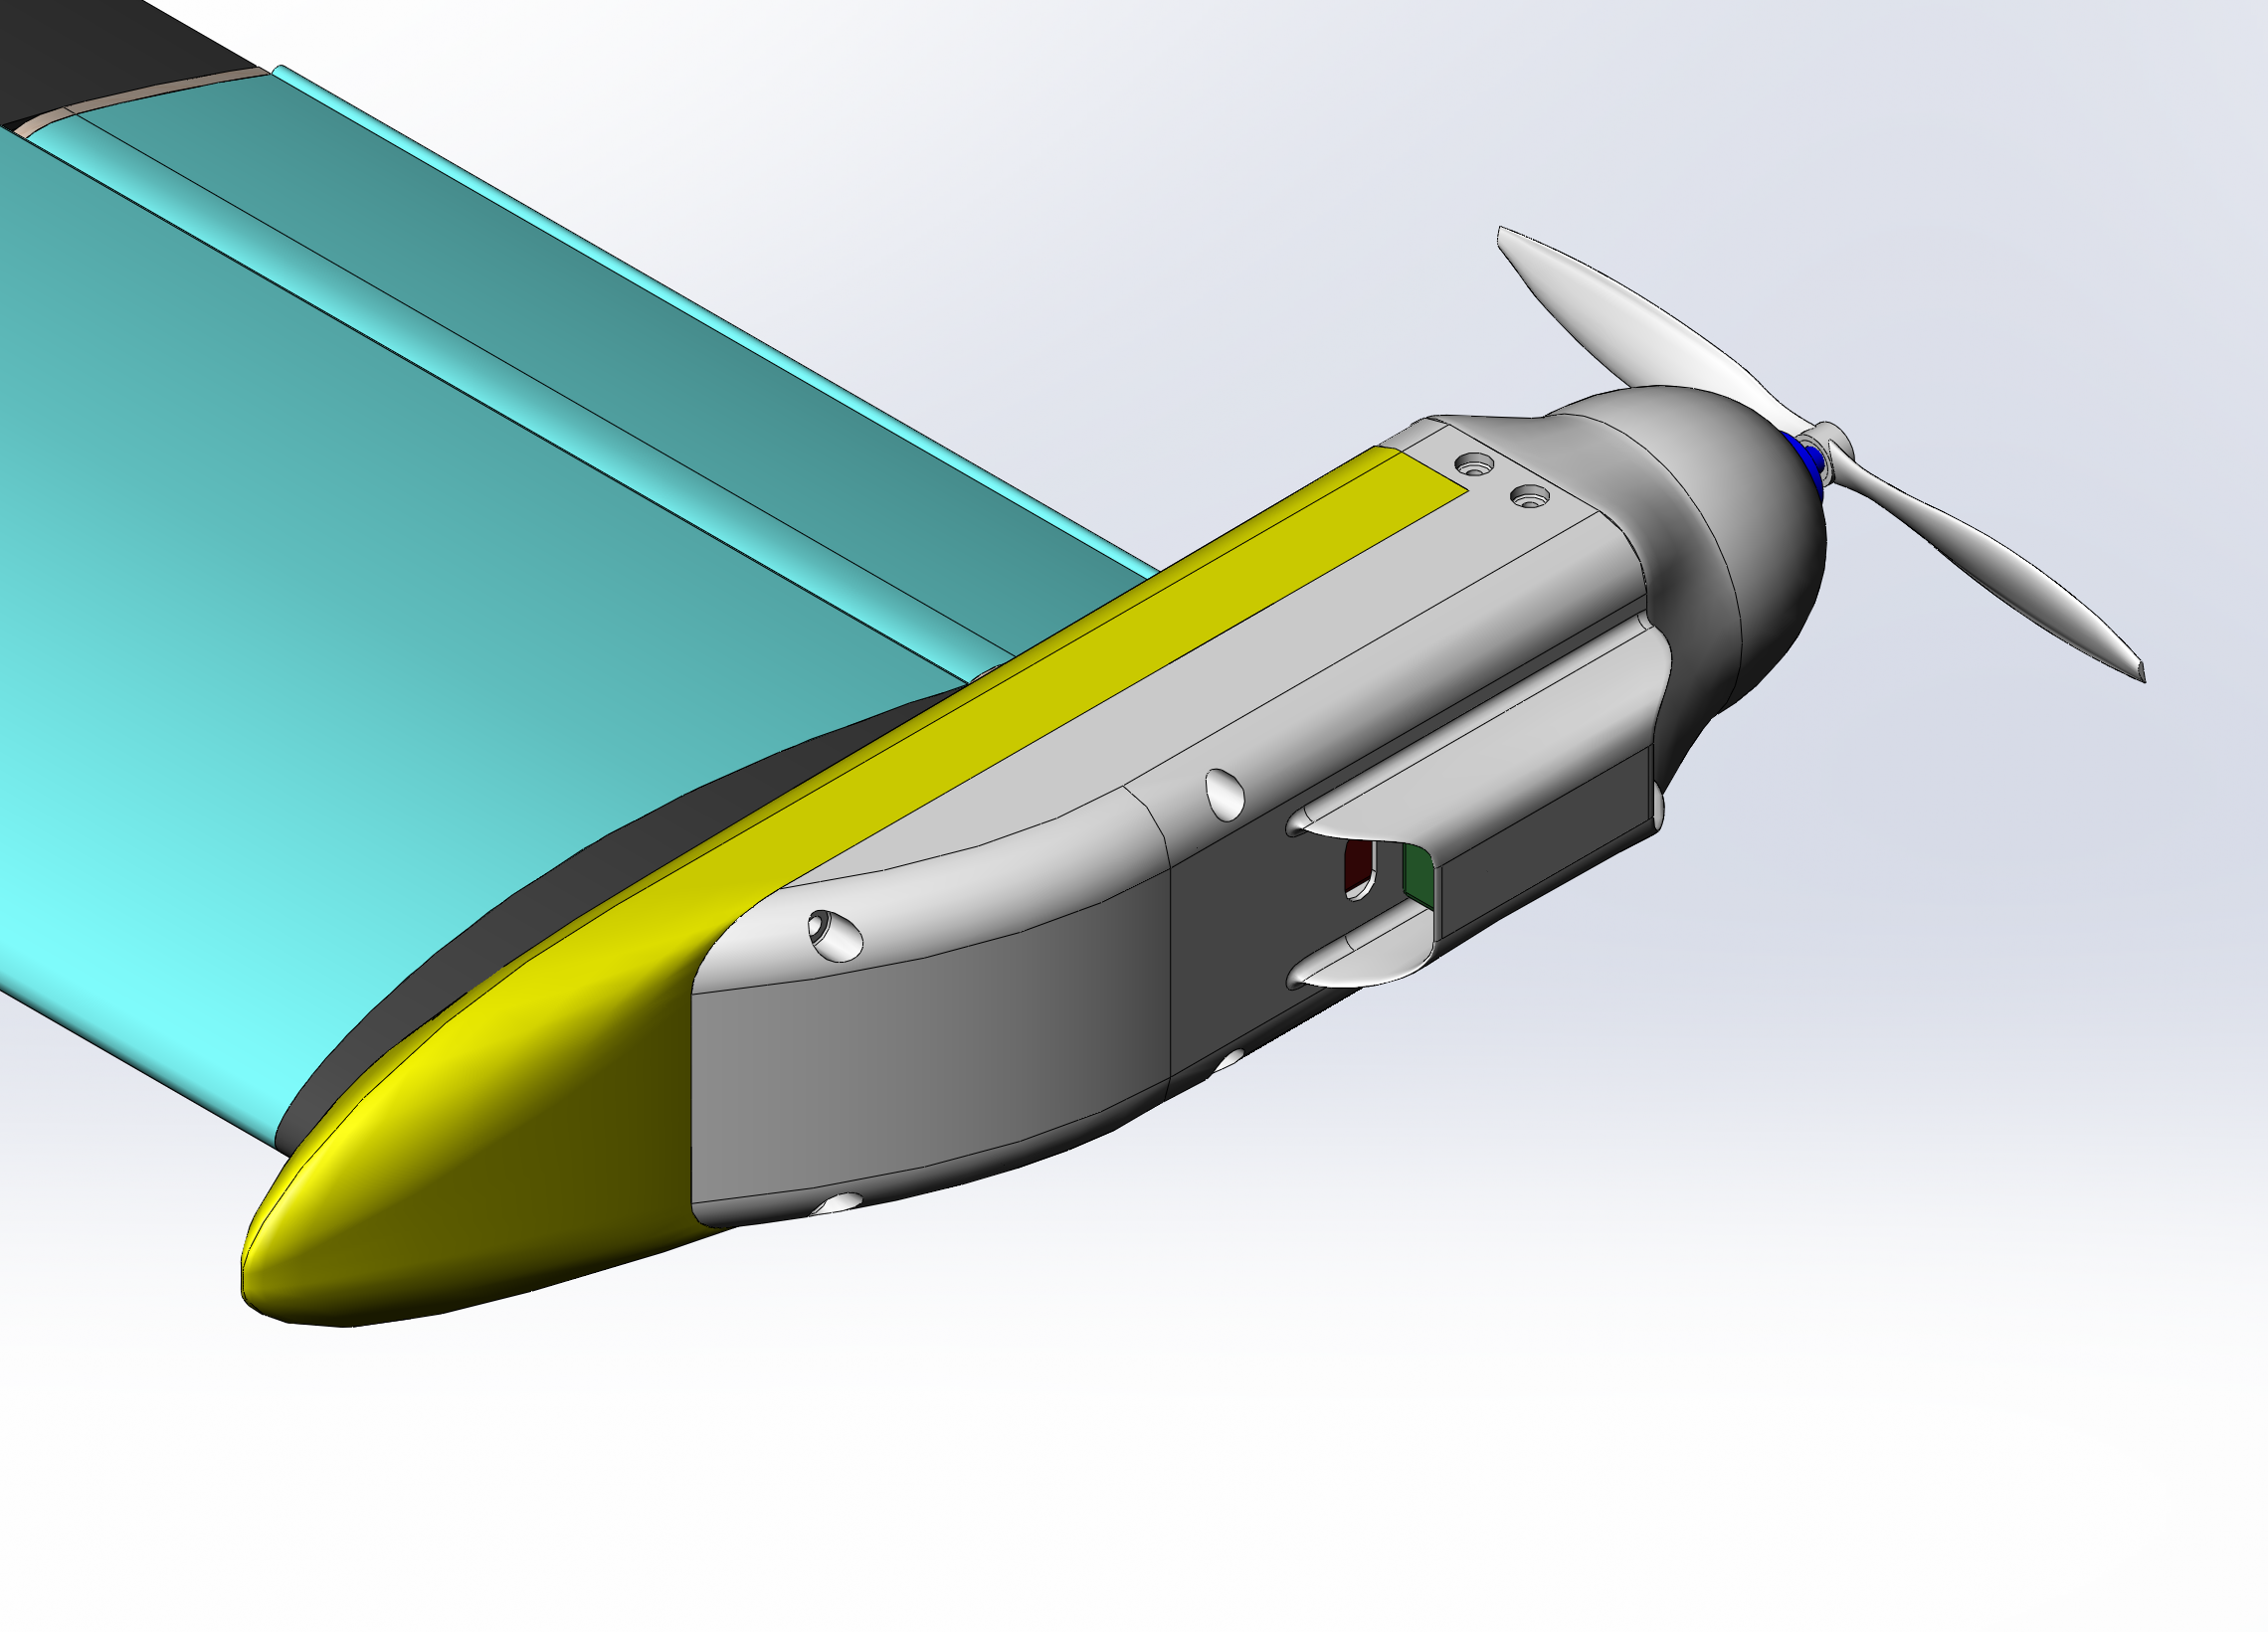
\includegraphics[width=\textwidth]{wingtip-pusher}
        \caption{Wingtip pusher}
        \label{fig:wing-mounting:wingtip-pusher}
    \end{subfigure}
    \hfill
    \begin{subfigure}[b]{0.49\columnwidth}
        \centering
        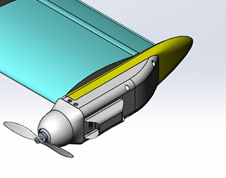
\includegraphics[width=\textwidth]{wingtip-tractor}
        \caption{Wingtip tractor}
        \label{fig:wing-mounting:wingtip-tractor}
    \end{subfigure}
    
    \caption{possible configurations of the PUC on the wing mounts.}
    \label{fig:wing-mounting}
\end{figure}

Each ‘mid-span’ insert in equipped four brass threaded inserts on both bottom and top surface.
These permit the fastening of the power unit cells and the respective adapter.
The location of the holes is the same for top and bottom surface (when viewed from the top).
Doing so, the same motor housing can be mounted on the top and bottom surface without alterations.
Furthermore, as presented in Fig. 5, the inserts are located at equal distance from the centreline positioned at half chord.
Thus, allowing the mounting of the same power unit cell in tractor or pusher configurations without the need for alterations. 

\importimage{wing-insert}{section view of the wing insert.}{Wing insert}{0.9}

The tip insert is designed so to mount the motor housing in horizontal position.
In order to use the same configuration of mounting points the tip adapter covers a structural role (unlike the rest).
This presents the brass inserts configuration discussed above so to guarantee the attachment of the standardized PUC.
The adapter is then mounted to the insert though two M6 bolts fastened to the two imbedded nuts shown in Fig. 2b. 

In order to reduce the elements composing the wing assembly, these components cover the function of ribs as well providing further torsional rigidity to the wing structure.
The two holes shown in Fig. 5 permit the carbon spars to run through the rib insert.
Thus, providing a secure attachment and sufficient bonding area.
Furthermore, as it will be later exposed, the housing for the active surfaces’ servos and flaps’ guides are designed to be integral part of the rib structure. 

\subsubsection{Mounting plate} \label{sec:design-process:final-design-proposal:wing:mounting-plate}

A Nylon printed mounting plate is located at the centre of the wing assembly.
This is tightly mounted to the wing spars so to guarantee a rigid support.
The wing assembly is then clamped onto the fuselage attachment plate through four M6 bolts.
These are positioned at the corners of the 3D printed plate as it is shown in Fig. 6.
A Styrofoam cover placed on top of the mounting plate is responsible for the blending of the wing assembly with the rest of the fuselage. 

\importimage{wing-assembly}{exploded view of the wing assembly attachment procedure}{Wing assembly attachment}{0.8}

The two cylinders housing the carbon spars ensure an even distribution of the loads though a large area (Fig. 7a).
This was essential since this component is subject to the totality of the load transferring from the wing to the fuselage and vice versa.
Therefore, extensive work was conducted using finite element analysis to generate a reliable and light design.
The peak loading for this component was established to be 4g, simulating an abrupt increase in lift Fig. 7b.
Hence producing the design shown in Fig. 7a. 

% \importimage{wing-plate-cad}{CAD representation of the wing mounting plate.}{Wing mounting plate CAD}{0.6}
% \importimage{wing-plate-fea}{stress concentration due to an applied load of 275 N.}{Wing mounting plate FEA}{0.6}

\begin{figure}[H]

    \centering
    \begin{subfigure}[b]{0.49\columnwidth}
        \centering
        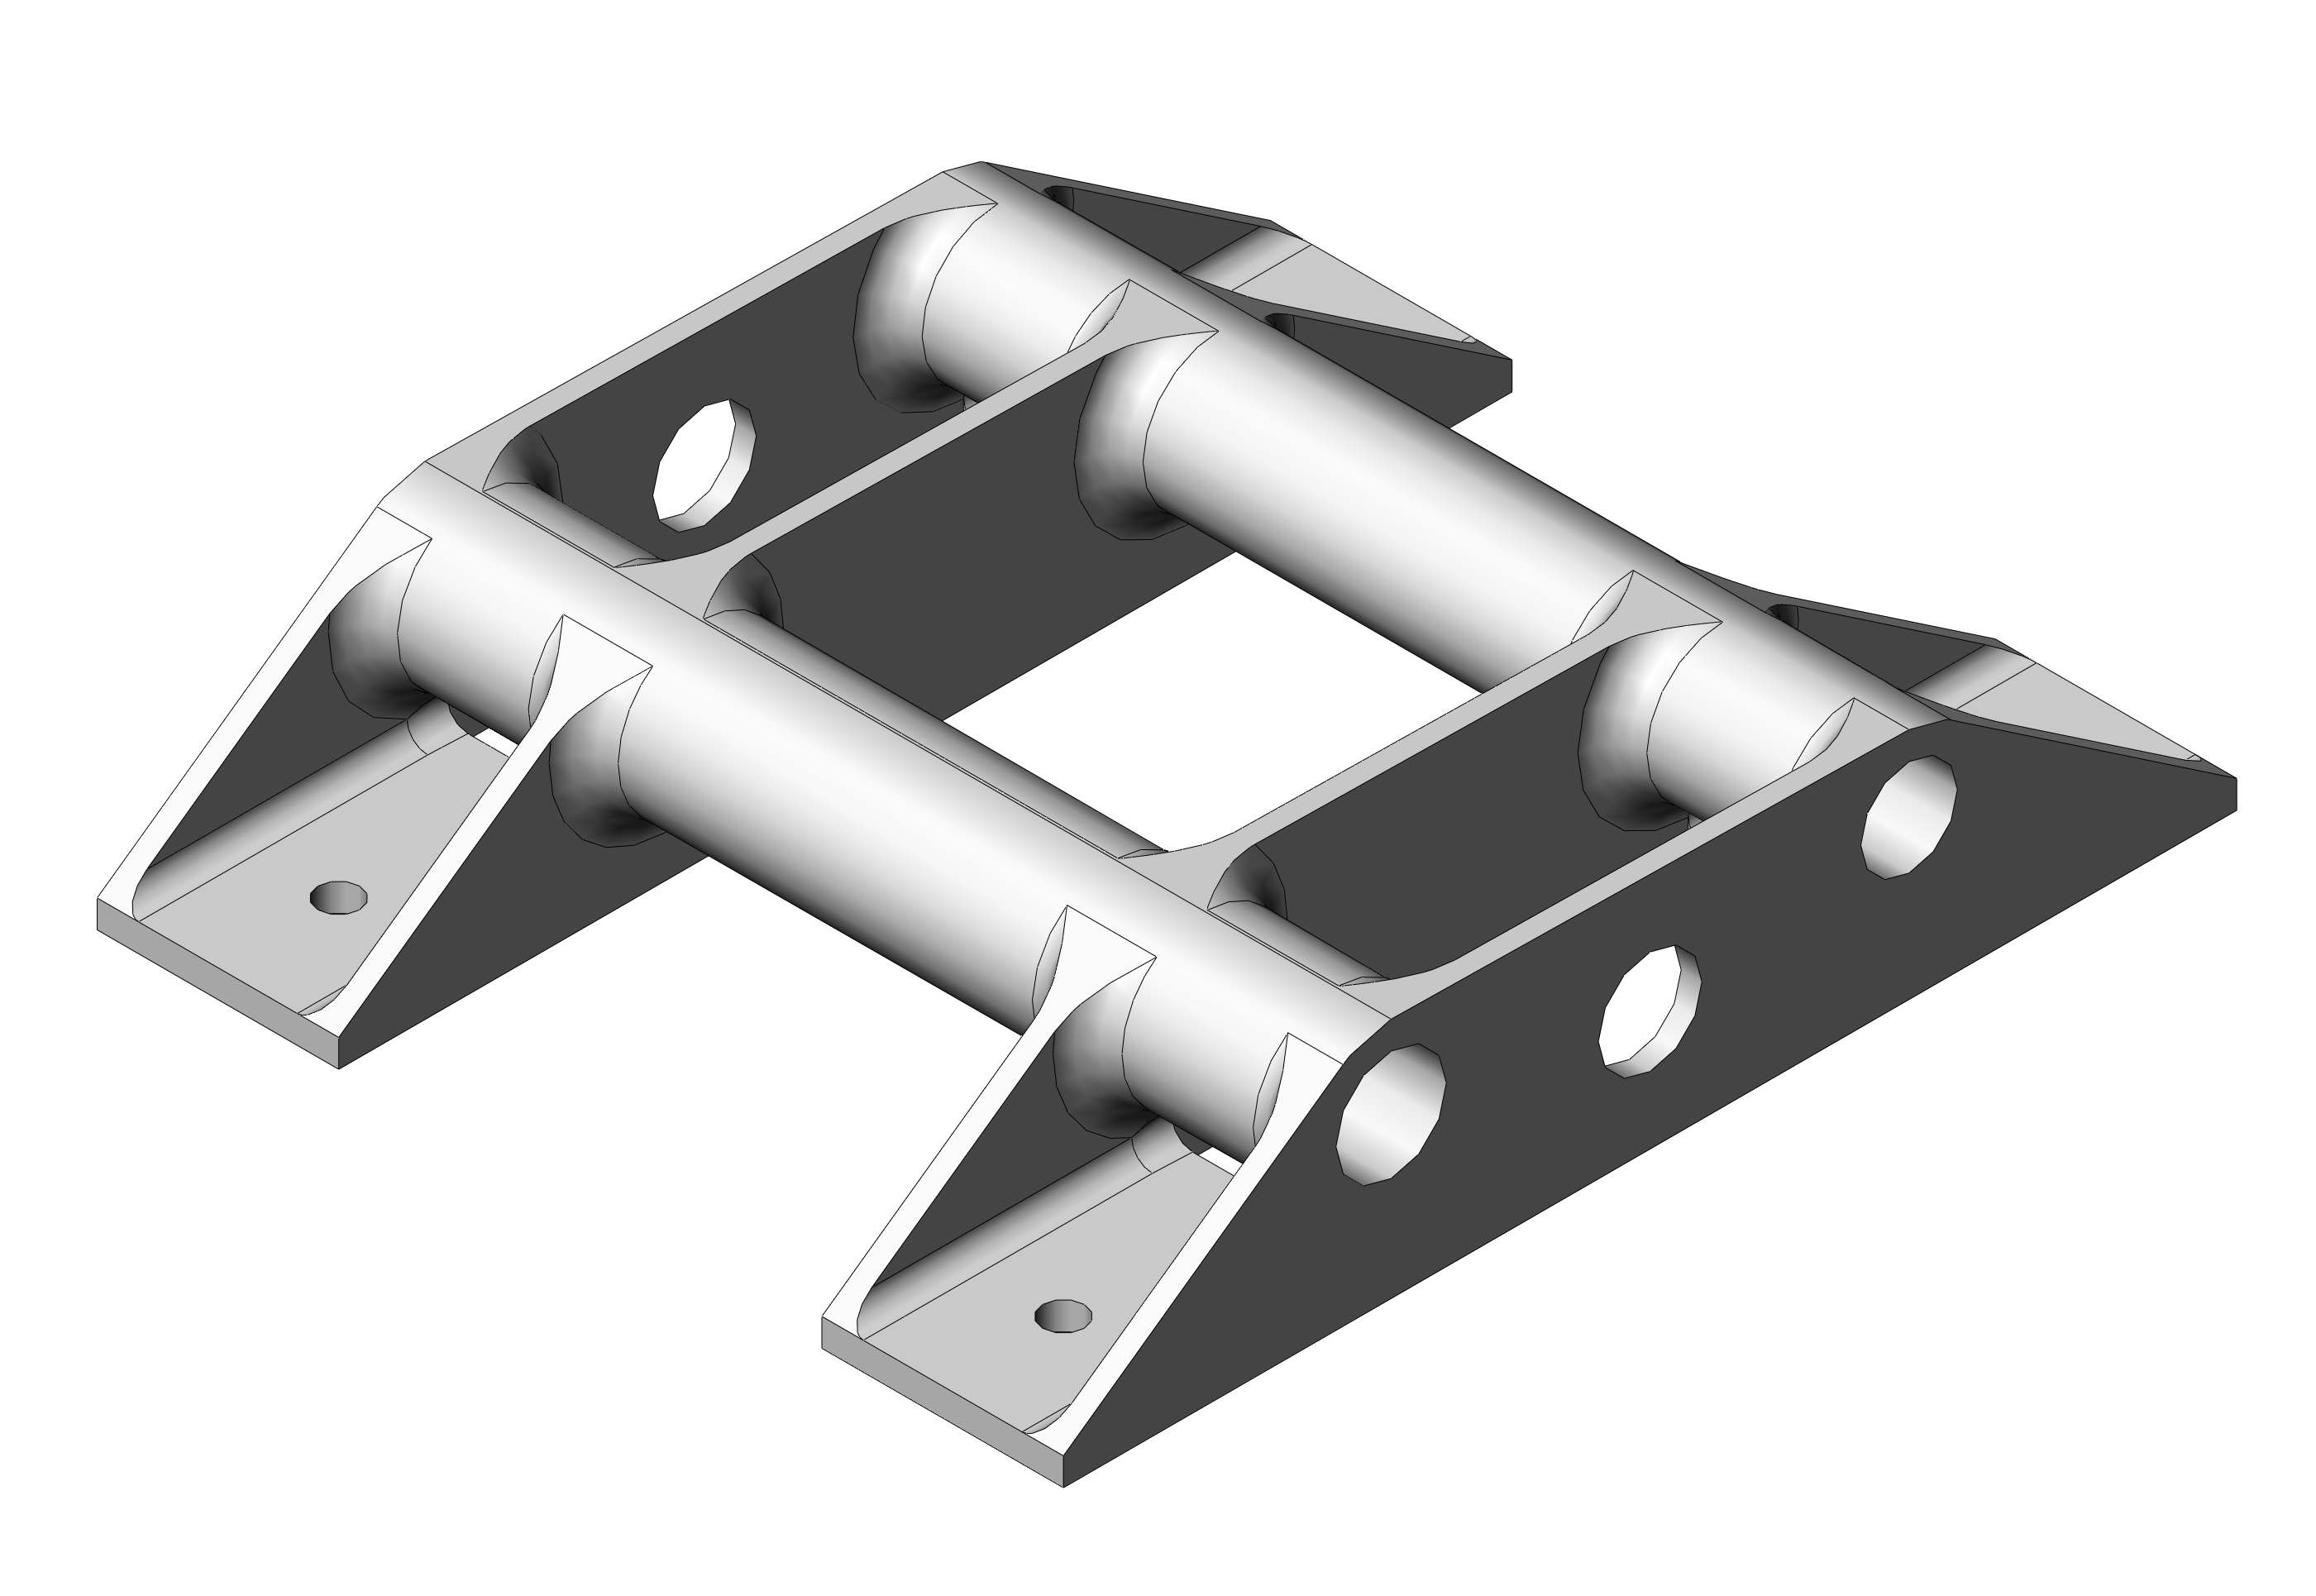
\includegraphics[width=\textwidth]{wing-plate-cad}
        \caption{CAD}
        \label{fig:wing-plate:cad}
    \end{subfigure}
    \hfill
    \begin{subfigure}[b]{0.49\columnwidth}
        \centering
        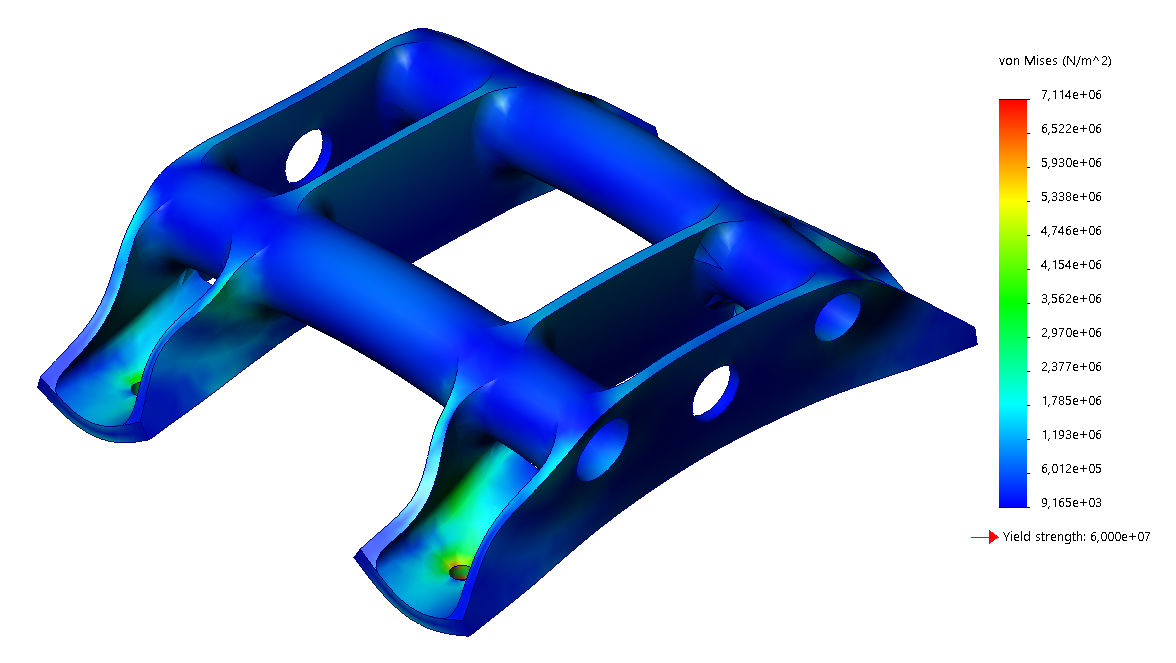
\includegraphics[width=\textwidth]{wing-plate-fea}
        \caption{FEA}
        \label{fig:wing-plate:fea}
    \end{subfigure}
    
    \caption{
        models of the wing mounting plate; (b) shows the stress concentration under a 275 N load.
    }
    \label{fig:wing-plate}
\end{figure}

\subsubsection{Flap mathematical modelling} \label{sec:design-process:final-design-proposal:wing:flap-mathematical-modelling}

Flaps were an obvious addition to aid take-off and landing.
It was decided to use single slotted flaps to increase flap efficiency and high lift capability.
The wing was split into three main sections between the motor mounts.
Because of the restrictions to span, the flap to wing chord ratios were the values that were altered to change high light performance.
It was also decided to use a small symmetrical deflection of the ailerons as the flaps were limited in performance.
It was considered to convert the trailing edges of the mounting locations into flaps too, however the increase in complexity led to the decision to ignore this idea. 

To begin, the flap geometry was parametrized by defining a chord ratio of the flaps to the wing, as well as the inboard and outboard spans of each flap.
The mathematical outcome of the process gave a required angle of the fuselage either on rotation or induced by a tail gear configuration, so work on the flaps aimed to reduce this angle, especially given the clearance required by the tail propeller demanding long landing gear legs. 

To mathematically model the flaps, first, a take-off speed was obtained from data provided by a teammate’s work on propulsion performance.
His initial calculation had provided a take-off speed of 10 m s-1 was not possible to design the flaps around with a reasonable required incidence.
After a dialogue, the take-off speed was agreed to be raised to 13 m s-1. 

To analyse the flap geometry, a process was devised from this authors own understanding, using flap parameters from M.
Sadraey’s book: ‘Aircraft design: A systems engineering perspective’.
According to table 5.15 in (Sadraey, 2013), the increase in local sectional lift coefficient for a slotted flap is 1.3 times the chord ratio of the flap to the wing, and the increase in local sectional lift coefficient for a plain flap (such as a converted aileron) is 0.7-0.9. 0.7 was selected out of this range to be conservative. 

It is important to note that this increase in lift coefficient is for a flap deflection of 60 degrees.
This is unrealistic for this application.
Additionally, because roll authority is required in all flight phases, so the full aileron deflection would not be usable for high lift gain, so a small angle of 5o downwards deflection was selected.
The maximum deflection of the slotted flaps was selected as 40o based on data in table 5.16 from (Sadraey, 2013).
The increase in lift coefficient for the respective flap was then multiplied by the ratio of the maximum deflection to 60o.
The value for the slotted flap was further multiplied by the chord ratio as required by the method. 

A simple version of the lift equation was then defined to account for the flap and aileron deflection at take-off: 

\importequation{
    \begin{aligned}
    L_{TO}  & {}= q S_{NoHLDs} (C_{L_0}+C_{L_\alpha}\alpha) \\
            & \quad + qS_f ((C_{L_0}+C_{L_\alpha}\alpha) + \Delta C_{L_f}) \\
            & \quad + qS_a ((C_{L_0}+C_{L_\alpha}\alpha) + \Delta C_{L_\alpha}) \\
            & {}= qSC_{L_0} + qSC{L_\alpha}\alpha + q S_a \Delta C_{L_\alpha} + q S_f \Delta C_{L_f}
    \end{aligned}
}{takeoff-lift}
% TODO: put line breaks into equation

which can be rearranged for $alpha$:

\importequation{\alpha = \frac{L_{TO} - q S C_{L_0} - q S_a \Delta C_{L_\alpha} - q S_f \Delta C_{L_f}}{q S C_{L_\alpha}}}{rearranged-takeoff-lift}

The take-off lift was estimated as 10 N greater than the maximum take-off weight of the UAV to provide responsive climb performance. Sa and Sf were determined by multiplying the total span for the flaps and ailerons by the wing chord, and $\Delta$CLa and $\Delta$CLf from the earlier calculations.
$\alpha$ resulted as 7.88o required wing total incidence on take-off, based on a final selected value of flap to wing chord ratio of 0.4, which was the maximum reasonable value before the flaps would begin impinging on electronics or wing spars.

The wing chord line had been set at an angle of 2o relative to the fuselage, the required incidence of the fuselage, either provided by the landing gear or rotation would be 7.8768o – 2o = 5.8768o. 

\subsubsection{Flap CAD} \label{sec:design-process:final-design-proposal:wing:flap-cad}

The shape of the flap was defined from a copy of the wing CAD.
Since a slotted flap had been chosen, a shroud from the wing had to extend to near the leading edge of the flaps in a deployed position such that boundary layer re-energisation on top of the flap would be optimal.
The wing shroud had been defined in CAD, so the profile of this was transferred onto the flap profile, smoothed out and then cut off from the leading edge and upper surface.  

Based on feedback on an original design, the flap mechanism of a Cessna-172 was selected as inspiration for the next version (Towell, 2019).
Images of this were studied, and a mechanism designed producing a smooth deployment both translationally back and down, and rotationally back to the 40 degree angle specified. 

\importimage{flap-mechanism-side}{the flap mechanism.}{Flap mechanism side view}{0.6}

The pins were made as central as possible in the flap so that they would not melt the walls of the flap in foam cutting.
These pins were also eventually changed to stiffening spars that would protrude beyond the end of the flaps to run along the tracks in the mechanism, but also stiffen the flap under aerodynamic loads.

% \importimage{retracted-flap}{retracted flap with endplates for horn controls.}{retracted-flap}{0.4}
% \importimage{deployed-flap}{deployed flap with endplates for horn controls.}{deployed-flap}{0.4}

\begin{figure}[H]

    \centering
    \begin{subfigure}[b]{0.49\columnwidth}
        \centering
        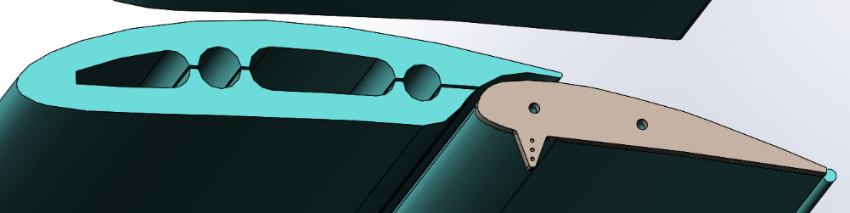
\includegraphics[width=\textwidth]{retracted-flap}
        \caption{Retracted}
        \label{fig:flaps:retracted}
    \end{subfigure}
    \hfill
    \begin{subfigure}[b]{0.49\columnwidth}
        \centering
        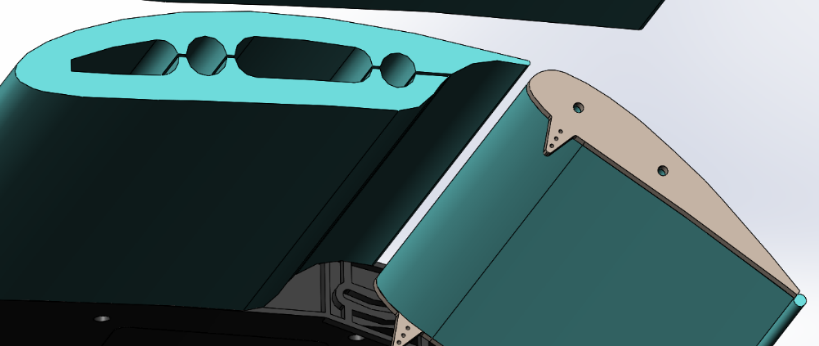
\includegraphics[width=\textwidth]{deployed-flap}
        \caption{Deployed}
        \label{fig:flaps:deployed}
    \end{subfigure}
    
    \caption{flap, with endplates for horn controls.}
    \label{fig:flaps}
\end{figure}

\subsection{Fuselage} \label{sec:design-process:final-design-proposal:fuselage}

\subsubsection{Central structure} \label{sec:design-process:final-design-proposal:fuselage:central-structure}

The main focus for the design of the UAV’s fuselage was to provide a reliable and simple platform for the experiments.
The concept for the design of the fuselage revolved around the idea of providing easy access to the electronics.
Changing the motor configuration multiple time demands the ability to check and modify the electronics with ease in order to proceed with the experiments in a smooth manner.
Therefore, the design presents a large electronics tray placed in the lower section of the fuselage; shown in purple in Fig. 8.
This can be accessed through the removal of the UAV’s nose.

\importimage{fuselage-inner-structure}{CAD representation of the inner structure of the fuselage's central section.}{Fuselage inner structure}{0.8}

All the fuselage’s structural components are located in the top section of this last.
Doing so a large area was created for the housing of the electronics as shown in Fig. 8.
The supports for the electronics tray, also referred as ‘fuselage ribs’, are designed to be manufactured out of 5mm birch wood sheets.
Such supports (represented in brown in Fig. 8), are mounted onto the fuselage central beam.
This is a square section carbon spar (20mm x 20mm) which extends for the entire fuselage length. 

A carbon fibre sandwich panel is placed onto the top surface of the fuselage’s central spar.
This is bonded at the wing’s attachment area with the aid of epoxy bonding agent.
In fact, its function is to provide the four mounting points for the bolts so to allow the fixing of the wing assembly to the fuselage.
The sandwich panel obtained by using a 5mm thickness nomex core placed between two carbon skins.
These last are each made out of 3ply woven carbon prepreg cured in autoclave.
Mounted below the plate are two PLA printed brackets (Fig. 9a); these are responsible for the correct positioning of the fuselage ribs and the landing gear mounting structure.
This is better shown in Fig. 9b.
Furthermore, they are designed to withstand a vertical load of 170N each; thus, offering a redundant attachment for the mounting plate in case of failure.

\importimage{pla-bracket}{CAD representation of the PLA bracket.}{PLA bracket}{0.5}
\importimage{brackets-highlighted}{fuselage central assembly with brackets highlighted in green.}{Highlighted brackets}{0.7}

\subsubsection{Landing gear attachment} \label{sec:design-process:final-design-proposal:fuselage:landing-gear-attachment}

The aircraft was design to not exceed 7kg of total mass.
Thus the position and the mass of the landing gear structure proved to be of significance in the position of the aircraft centre of gravity.
The ideal position of this was set to be at 50\% of the wing’s chord length; with a 5\% shift caused by the change in propulsion configuration.
The landing gear is mounted on two ‘C’ shaped 5mm aluminium brackets.
These are mounted to two bulkheads as shown in Fig. 10a.
These last cover the role of transferring and absorbing the vertical loads encountered during taxi, take off and landing.
In order to minimize the weight of this structure the bulkheads are designed to be manufactured as carbon fibre sandwich panels.
These have been specified to withstand vertical loads up to 5g.
Furthermore, two triangular braces, as shown in Fig. 10b, are attached to the lowest section of the bulkheads and are clamped to the main spar through a PLA insert.
These work in compression and are designed to counteract the moments generated by the loads acting on the wheels in the direction of travel. 

% \importimage{landing-gear-attachment}{landing gear attachment structure.}{Landing gear attachment}{0.4}
% \importimage{landing-gear-side}{landing gear attachment side view.}{Landing gear attachment side view}{0.4}

\begin{figure}[H]

    \centering
    \begin{subfigure}[b]{0.4\columnwidth}
        \centering
        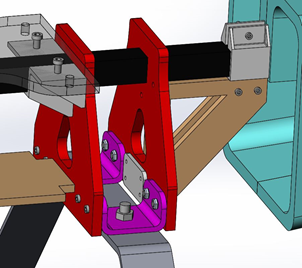
\includegraphics[width=\textwidth]{landing-gear-attachment}
        \caption{}
        \label{fig:landing-gear-attachment:angled}
    \end{subfigure}
    \hfill
    \begin{subfigure}[b]{0.49\columnwidth}
        \centering
        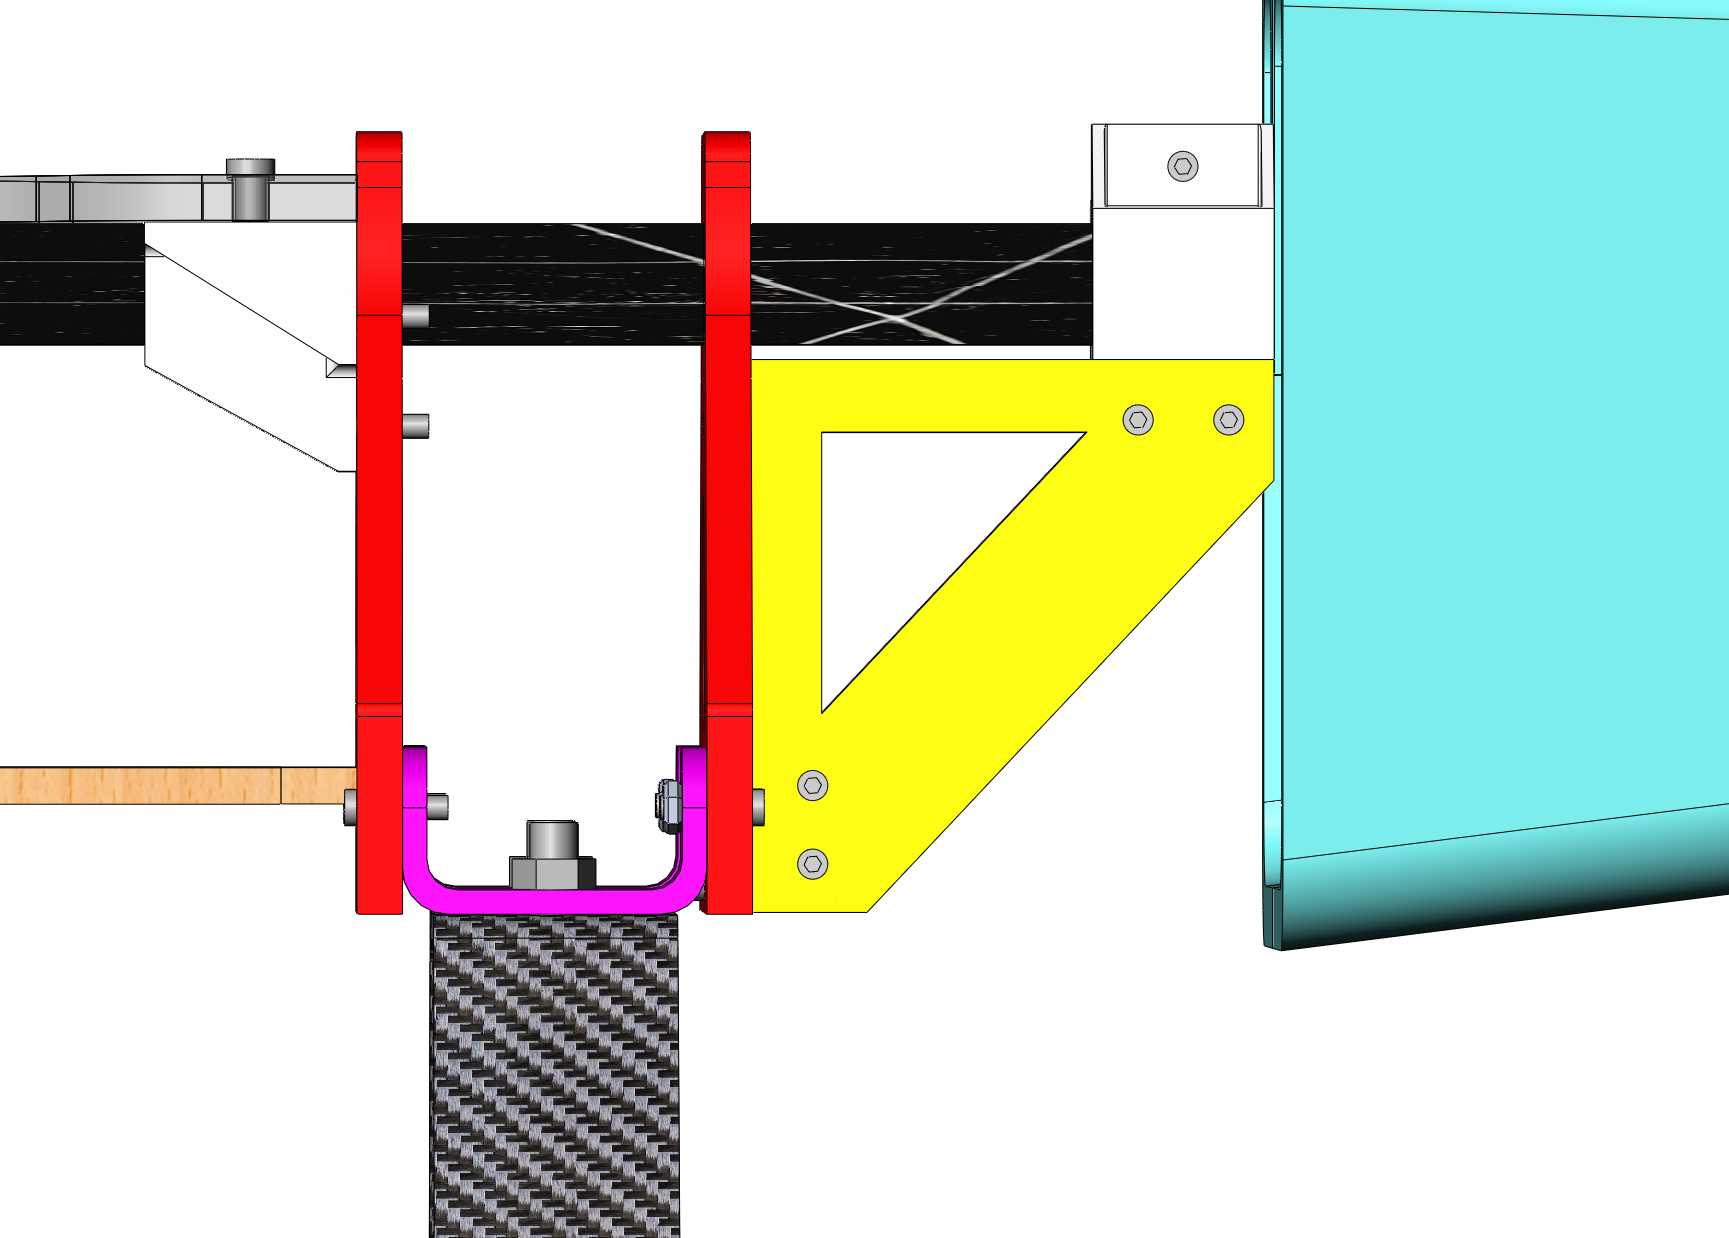
\includegraphics[width=\textwidth]{landing-gear-side}
        \caption{}
        \label{fig:landing-gear-attachment:side}
    \end{subfigure}
    
    \caption{landing gear attachment structure.}
    \label{fig:landing-gear-attachment}
\end{figure}

The carbon fibre sandwich panels bulkheads are design in the same manner as the fuselage central plate discussed previously.
A schematic of this is provided in Fig. 11. 

\importimage{carbon-fibre-sandwich}{CAD representation of the carbon fibre sandwich panel components.}{Carbon fibre sandwich}{0.5}

\subsubsection{Finite element analysis} \label{sec:design-process:final-design-proposal:fuselage:finite-element-analysis}

In order to verify the strength of the design and identify any weak points, some FEA was carried out using the Simulation function in SolidWorks.
This is a fairly basic FEA system and can only use coarse meshes otherwise the simulations fail, but it gives a good indication of the strong and weak areas of the fuselage design.
The materials of the parts of the fuselage were all specified and the data for those materials applied as accurately as possible in order to ensure the parts relative strengths were reflected in the simulations.
The model is stripped down to the minimum components required to perform the simulations in order to save computational time and simplify the simulations.
Initially a simulation was run to test the effects of high turning loads, with the main tail boom fixed in place as the reference point of the study and loads of 210N applied vertically upwards on the wing spar holes in the wing mount, and 80N applied vertically down on the component tray.
These loads were chosen to simulate 3g loads in a turn, with the mass of the components assumed evenly distributed over the tray.
Figure 1 shows the results.

\importimage{fuselage-stress-distribution}{fuselage stress distribution during a simulated 3g turn.}{Fuselage stress distribution}{0.7}

It can be seen that the wing mount shows that the maximum stress experienced is around 1.6 MPa, which is significantly below the 30 MPa yield stress of the ABS material used.
The other high stress locations are on the lower parts of the component tray mounts, which peak at over 2 MPa, but the plywood used has a yield stress of 30 MPa and so this is also well below the point of breaking.
It can also be seen that the stress on the carbon fibre tail boom reaches over 2 MPa, but this is well below the yield stress of the carbon tube which will be over 600 MPa based on the properties quoted at [Performance Composites [REF]]. 

The second simulation is showing the effects of landing loads, with the tail boom again fixed and the loads applied at the locations of the wheel centres on the landing gear.
This simulation only tests the main gear as this is where the highest forces should be experienced if the UAV is landed properly.
The forces applied are 350N vertically up and 105N horizontally rearwards to simulate a heavy landing of 5g with 1.5g deceleration force. 

\importimage{landing-leg-simulation}{simulated stress distribution over one of the landing legs.}{Landing leg simulation}{0.4}
\importimage{fuselage-landing-simulation}{stress distribution over the fuselage during a simulated landing.}{Fuselage landing simulation}{0.6}

It can be seen in Figure 2 that the peak loads experienced by the landing gear are around 260MPa, which is below the yield stress of the carbon fibre as previously stated, and although it is nearing the yield stress, this is an extreme case of a particularly heavy landing and so a heavier landing than this would not be expected unless it occurs in a crash landing scenario in which case the UAV surviving would be down to luck.
It can also be seen that the peak stress on the landing gear brackets is around 100MPa, below the yield stress of around 270MPa of the aluminium they are made of.
With the scale modified to a reduced upper bound, the stresses on the other parts can be seen, with the peak stress experienced by the landing gear mounts seen as around 10 MPa, which is massively below the yield stress of carbon fibre and although the properties of carbon fibre sandwich panel are varied, they are quoted as having a yield stress of at least 100 MPa, and so this is not close to failure. 

\subsection{Landing gear} \label{sec:design-process:final-design-proposal:landing-gear}

There are two main types of landing gear design considered for this project: the tricycle and a tail wheel approach. A tricycle consists of a single front wheel, and two rear wheels, as seen on most commercial aircraft.
Whereas a tail wheel design uses a single rear wheel with two front wheels.

\importtable{| >{\raggedright\arraybackslash}p{0.12\columnwidth} | >{\raggedright\arraybackslash}p{0.36\columnwidth} | >{\raggedright\arraybackslash}p{0.36\columnwidth} |}{
    \hline
    \textbf{Design} & \textbf{Advantages} & \textbf{Disadvantages} \\
    \hline
    Tricycle & Prevents nose tipping; improved stability; better manoeuvrability; better in crosswinds & Increased drag and weight; nose gears are prone to damage \\
    \hline
    Tail wheel & Lighter; easier to integrate with under rudder; more suitable for integration with nose design; propellors would have more ground clearance & Harder to attach front wheels; harder to manoeuvre \\
    \hline
}{tradeoffs involved in the gear layout used.}{gear-layout-tradeoffs}

When the landing gear was first being designed  weight was the limiting factor, with the UAV close to the 7kg mass limit, because of this the decision was made to use a tail wheel approach as it is lighter than the tricycle approach.

The modularity and moving centre of gravity was a unique challenge to this UAV.
The first step of the design was the calculation of the maximum loading conditions the landing gear would encounter (Goud, 2014). 

\importimage{moment-calculations}{moment calculations.}{Moment calculations}{0.7}

The forward most CG meant x=150mm and y=765mm, this led to a maximum static loading of 57.4N over the front wheels and 11.26N over the rear wheel.
The rearmost CG led to x=200mm and y=815mm, the maximum static loadings for this condition is 55.13N and 13.53N over the front and rear wheels, respectively.
Based on these calculations, a load of 57.4N and 13.53N were used in future calculations and analysis. 

A vertical velocity of 3m/s was assumed to be an aggressive landing velocity in the hands of a competent pilot and was used in calculation to ensure the landing gear would be strong enough to withstand multiple rough landings.
Using Newtons 2nd law, and an assume impact time of 0.5 seconds, the maximum force of the UAV is equal to 42N, meaning a total force of 110.67N on landing.
Most UAVs land with their main wheels touching down first, the main landing gear must absorb most of the load, on previous calculations the main gear should withstand 99.4N.  

\importimage{landing-gear-design-one}{landing gear design one.}{Landing gear design}{0.8}

A setting angle of 5.8degrees was needed to meet take-off requirements, as shown in figure 1.
To avoid hitting the rear propeller or the rudder, the rear wheel was designed to extrude from the bottom of the under-rudder.
The carbon fibre spar in the rudder would be string enough to support the maximum 10N load it would encounter on landing. 

\importimage{landing-gear-attachment-locations}{potential landing gear attachment locations.}{Landing gear attachment locations}{0.7}

It immediately became clear that the main gear would have to be mounted to the main carbon fibre boom running the length of the fuselage.
However, after a supervisor meeting it was advised that the main wheels should be located below the leading edge of the wing.
However, as figure 2 shows, mounting the main gear would not be possible in this location.
A solution to have the main gear mounted further forward but curved backwards was devised.  

Several iterations similar to the final design, in figure 3, were designed and tested using FEA.
The FEA was initially carried out on a single leg, with a loading of 50N applied to a fiberglass construction.
After the design of the leg was finalised a clamping system was devised to mount the main gear to the boom.
Further FEA showed that the clamping would be effective at attaching the fibreglass to the boom but would cause the boom to buckle on landing.
Figure 5 shows how the addition of a prepreg cover around the boom significantly reduces the stress of the boom itself, by roughly a factor of 10. 

% \importimage{landing-gear-design}{main landing gear design.}{Landing gear design}{0.4}
\importimage{landing-gear-stress}{stress on landing gear.}{Landing gear stress}{0.5}
\importimage{prepreg-cover-stress}{effect of a prepreg cover on carbon fibre spar.}{Prepreg cover stress}{0.95}

At this point in the design process, the weight of the UAV was no longer an issue, and after a supervisor meeting in which the landing gear design was discussed, it was decided that the landing gear should be steerable.
This would reduce time to retrieve the UAV on landing as well as making take-off easier.
The tail wheel set up is not optimum for a steerable configuration.
Therefore, as the fuselage and the weight of the aircraft had been reduced making weight less of an important factor, the decision was made to redesign the landing gear in a tricycle configuration. 

\begin{figure}[H]
    \centering
    \begin{subfigure}[b]{0.33\columnwidth}
        \centering
        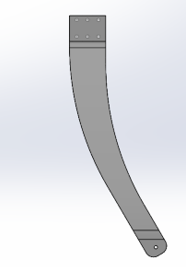
\includegraphics[width=\textwidth]{landing-gear-design}
        \caption{Initial}
        \label{fig:main-gear-progression:initial}
    \end{subfigure}
    \hfill
    \begin{subfigure}[b]{0.49\columnwidth}
        \centering
        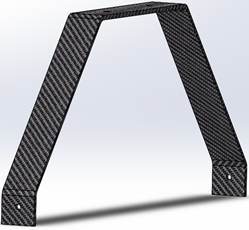
\includegraphics[width=\textwidth]{main-gear-design}
        \caption{Final}
        \label{fig:main-gear-progression:final}
    \end{subfigure}
    
    \caption{progression of the main gear design.}
    \label{fig:main-gear-progression}
\end{figure}

Using a similar process to the tail wheel design, the main landing gear was calculated to experience up to 105.8N on landing.
The main gear is now located behind the centre of gravity, behind the internal electronics.
This, along with a redesigned fuselage means the landing gear could be designed as a single part and attached easily to the bottom of the fuselage. 

% \importimage{main-gear-design}{main gear design.}{Main gear design}{0.4}
\importimage{main-gear-fea}{main gear FEA stress results.}{Main gear FEA}{0.6}

The main shape of the design didn’t change from the initial design, a similar design which is seen on many small UAVs as it is simple, easy to implement and robust.
FEA was carried out on the design and small changes made until an optimum design was found.
The final design would experience a maximum stress of 92.5Mpa on a rough landing.
The final design would later be manufactured from carbon fibre because it can be manufactured cheaply on at university and it has a high strength to weight ratio.
The knowledge of this manufacturing decision gave more freedom to the design.
The final design had a maximum thickness of 6mm at the top where it joins the fuselage, narrowing to 4mm by the wheels.
The depth remained constant at 65mm, with a wheelbase of 490mm and a height of 220mm this was to avoid hitting the under rudder on take-off.
The redesigned fuselage structure with two lower plates meant the landing gear could easily be mounted to the fuselage using two M4 bolts. 

Before manufacturing began on the component, a similar model was found online. A cost benefit analysis was carried out, along with a time benefit analysis, and it was determined that purchasing the landing gear would allow the focus on other areas of design that needed finalising. 

\importimage{landing-gear-join}{landing gear joining mechanism.}{Landing gear joining mechanism}{0.6}

The nose gear was chosen at recommendation of co supervisor Mario Ferraro, it is the same at that used on the SPOTTER aircraft, a 24kg split fuselage UAV (SPOTTER, 2019). It was easy to implement into the nose design and make steerable, whilst being cheap, lightweight, and strong. 

\subsection{Nose} \label{sec:design-process:final-design-proposal:nose}

The nose was a key component in the project and needed to fulfil several criteria:

\begin{itemize}
    \item support a motor and propellor unit;
    \item provide access to the motor for removal;
    \item be removable from the rest of the fuselage whilst being strong enough to support the motor during flight;
    \item integrate the landing gear.
\end{itemize}

To fulfil all the above criteria, it was obvious from the start that the nose would have to be 3D printed, this meant there were no restrictions regarding the design.  

The initial design was simple, incorporated the ability to attach the motor via four internal screw holes.
The nose would be attached to the fuselage via a spar running through the nose and the front of the spar.
Although not optimal, at the time it was deemed acceptable to drill through the end of the carbon spar as it was away from the structural core of the fuselage.
The design also incorporated a slot for the battery to slide into to act as a ballast, as well as a slot for the ESC which would maximise airflow to it therefore cooling.

\begin{figure}[H]
    \centering
    \begin{subfigure}[b]{0.6\columnwidth}
        \centering
        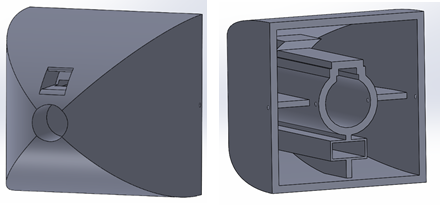
\includegraphics[width=\textwidth]{initial-nose-design}
        \caption{Initial}
        \label{fig:nose-design-progression:initial}
    \end{subfigure}
    
    \begin{subfigure}[b]{0.6\columnwidth}
        \centering
        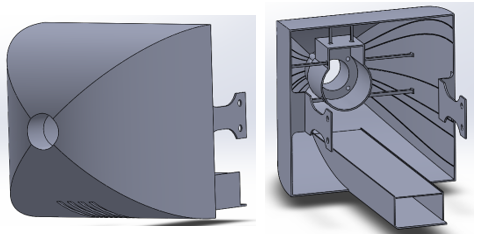
\includegraphics[width=\textwidth]{revised-nose-design}
        \caption{Revised}
        \label{fig:nose-design-progression:revised}
    \end{subfigure}

    \begin{subfigure}[b]{0.6\columnwidth}
        \centering
        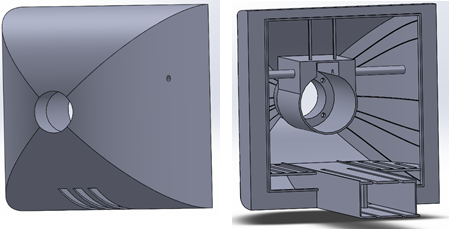
\includegraphics[width=\textwidth]{twice-revised-nose}
        \caption{Final}
        \label{fig:nose-design-progression:final}
    \end{subfigure}
    
    \caption{various stages of the design of the printed nose.}
    \label{fig:nose-design-progression}
\end{figure} 

% \importimage{initial-nose-design}{initial nose design.}{Initial nose design}{0.6}

Figure 11 shows a redesigned model of the nose.
Firstly, the outer body has been light weighted considerably from 5mm to 1.5mm and supports added.
The battery compartment has become a tray, which will make removal easier.
The tray has a section underneath for the ESC to be placed, with cooling vents in the front of the nose.
The nose will be secured to the fuselage via two bolts the width of the fuselage.
More light weighting was done to the motor support and rods used instead of the previous bulky design. 

% \importimage{revised-nose-design}{revised nose design.}{Revised nose design}{0.7}

After advice from our supervisor, alterations were made to the initial design.
Noticeably a battery and ESC tray was added to the back of the nose, with vents in the front of the nose to allow cooling to the ESC.
The tray was supported by two vertical poles to support the weight of the battery. 

% \importimage{twice-revised-nose}{twice revised nose design.}{Twice revised nose design}{0.7}

The nose would now be secured by one bolt, through the carbon fibre spar, this would also act as a support for the motor mount as well.
However, after further deliberation with our supervisor, it was decided that the loss I structural performance from drilling through the carbon fibre boom was not worth the reduction in workload so a new way of attaching the nose to the fuselage needed to be devised.  

The new nose design had two components.
The inner component would be secured to the fuselage at all times, and the front part would be removeable.
The inner part would be secured to the boom using a clamping mechanism, originally devised for the landing gear, via three M3 bolts located underneath the boom.
The outer part would then twist into the inner part then be locked in place using two M3 bolts. 

\begin{figure}[H]
    \centering
    \begin{subfigure}[b]{0.6\columnwidth}
        \centering
        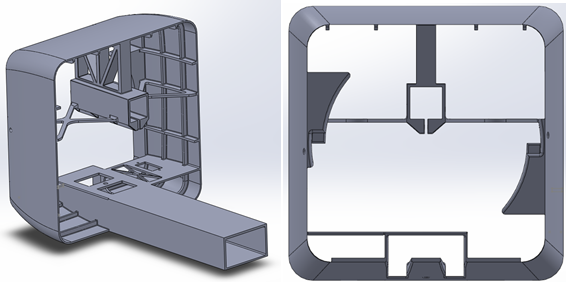
\includegraphics[width=\textwidth]{nose-inner-section}
        \caption{Inner section}
        \label{fig:nose-design:inner}
    \end{subfigure}
    
    \begin{subfigure}[b]{0.6\columnwidth}
        \centering
        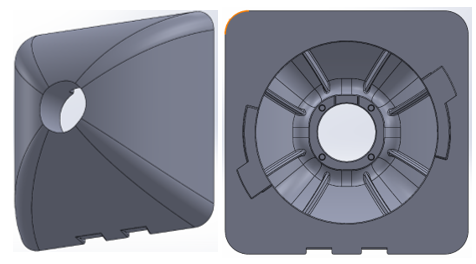
\includegraphics[width=\textwidth]{nose-outer-section}
        \caption{Outer section}
        \label{fig:nose-design:outer}
    \end{subfigure}

    \begin{subfigure}[b]{0.6\columnwidth}
        \centering
        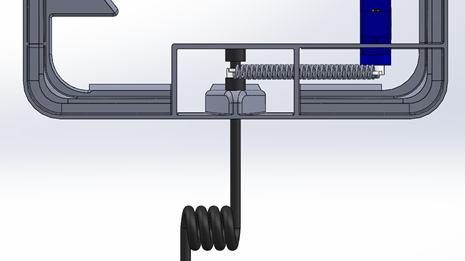
\includegraphics[width=\textwidth]{steerable-gear}
        \caption{Steerable gear attachment}
        \label{fig:nose-design:steerable-nose-gear}
    \end{subfigure}
    
    \caption{detailed models of the final nose design.}
    \label{fig:nose-design}
\end{figure} 

% \importimage{nose-inner-section}{inner section of the nose.}{Nose inner section}{0.7}

The inner part would have a 1mm wall thickness, supported by 5mm deep and 3mm wide support structures, this is common on 3D printed UAV components as it is a light way of adding strength.
The clamping system is supported by a web like structure.
The battery tray and ESC compartment had a small redesign, two larger vents channelling airflow to the ESC.
The steerable landing gear has also been incorporated into the design, through the air vents. 

% \importimage{nose-outer-section}{outer section of the nose.}{Nose outer section}{0.7}

The outer section will be held in place via a twist and lock system.
To remove the front section two screws will be removed from the side of the nose, the front will then twist anticlockwise and be removed.
Once removed, the electronics inside will be removed easily over the battery tray.
The motor can easily be removed via 4 screws located towards the front of the nose and replaced by a 3D printed part for when not in use.
The motor mount area has also been lightened, will similar structural supports on the 1mm outer wall applied. 

\importimage{outer-nose-fea}{FEA on the outer nose join.}{Nose join FEA}{0.7}

FEA was carried out on the outer section to ensure it was strong enough to support the fuselage.
Figure 13 shows a 140N force applied to the locking tabs.
For SLS Nylon the yield strength was set at 60Mpa.
However, with the 140N load applied, the maximum stress reached was 5.582MPa, and a maximum displacement of 0.1mm. 

Having fulfilled the first three criteria, the final design also incorporates a steerable landing gear.
This part of the design was thought about throughout the design process, but only fully implemented after the landing gear design had been finalised. 

% \importimage{steerable-gear}{integration of the steerable nose gear.}{Steerable nose gear}{0.7}

Figure 16 shows how the nose gear would have been incorporated within the vent design.
The nose gear would be secured using two collars, one above and below the thicker part of the nose, as well as one to secure the servo arm in place.
The servo arm would be attached to the servo via two springs, these will reduce the impacts and prevent the nose from rapid direction changes due to bumps.
The servo will be bolted onto the battery tray, to one side, to allow space for the battery tray to be removed. 

As stated during the landing gear analysis, depending on the configuration, will have to withstand a force of up to around 35N on landing.
Therefore, FEA was carried out on the nose.
The results show a moderate level of stress on the wall at the bottom of the vent; however, this was about half of the perceived yield strength of the SLS nylon which would be used. 

\importimage{nose-connection-fea}{FEA on nose and landing gear connection.}{Nose connection FEA}{0.7}

When the nose motor was not needed it was removed and replaced with a small insert.
The hollow insert would have been 3D printed on the university 3D printer using PLA as it is not a structural component.
It was designed to be screwed in the same manner as the motor. 

\importimage{nose-motor-filler}{nose motor filler.}{Nose motor filler}{0.5}

\subsection{Tail} \label{sec:design-process:final-design-proposal:tail}

\subsubsection{Mathematical modelling} \label{sec:design-process:final-design-proposal:tail:mathematical-modelling}

The tail needs to provide adequate stability to the aircraft in all stages of flight, as well as house the elevator and rudder control surfaces.
Design for the tail and stability systems essentially re-started following research and dialogue with our supervisor after the wing tunnel test, which revealed the true scope of the design process required. 

Design began with the tail surfaces themselves.
As the centre of gravity of the aircraft would not be in line with the centre of lift, the tailplane would need an angle of attack that would facilitate the aircrafts stability throughout flight, with minimal to no trim from the elevators.
The sizing of the tail surfaces, and their angles were again determined using processes from (Sadraey, 2013).
In particular an example of tail design was followed from section 6.1 (and slightly modified) to obtain the tail dimensions and setting angle. 

The process began similarly as that of the wind tunnel model.
Revised volume coefficients were suggested as 0.8 for the horizontal tail, and 0.06 for the vertical tail (Towell, 2019).
Equations [1] and [2], were used to determine the tail planform area as 0.16 m2 for the horizontal tail, and 0.08 m2 for the vertical tail.  

Next the cruise lift coefficient was determined, using equation 6.27 from (Sadraey, 2013) and was found to be 0.4671, based on a weight of 7g (68.67 N), cruise speed of 20 m s-1 and wing planform area of 0.6 m2.
Next the wing/fuselage aerodynamic pitching moment coefficient required estimating.
Sadraey’s book provided an equation for this, however at the suggestion of Prof. Towell, equation E-40, which determined the change in wing pitching moment due to the fuselage, from E. Torenbeek’s book, ‘Synthesis of Subsonic Airplane Design’ (Torenbeek, 1976).
This was determined to be -0.0398.
Based on a chart from ‘Airfoil Tools’ for the NACA 6412 aerofoil, the wing 0 lift pitching moment coefficient was determined to be -0.137 (Airfoil Tools, 2020).
Then, this and the fuselage offset were summed to give a value of the wing/fuselage pitch moment coefficient of -0.1768. 

The next stage of the process required values for the centre of lift and mass locations in terms of percent of the MAC of the wing.
As these were unknown at this stage, they were estimated to be h = 0.25 (quarter chord) for the centre of lift (a reasonable assumption for most wings) and h0 = 0.5 (half chord) for the centre of mass, which was a worst case value. 

Next, the required lift coefficient of the horizontal tailplane was required.
Essentially, the moment caused by the lift, thrust and weight, as well as the wing pitching moment has to be counteracted by a moment provided by the tail.
It was decided that this should be negated at the cruise speed of the UAV, reducing the work required by the pilot for the bulk of the flight.
The tail uses a symmetrical aerofoil, and as such provides no lift force at 0 incidence, so requires a mounting angle to provide a balancing moment.
However, this has to take into account changes to flow incidence caused by the fuselage angle of attack at cruise to make the wing provide sufficient weight balancing lift, as well as flow downwash caused by the wing. 

To calculate the tail cruise lift coefficient, (Sadraey, 2013) provided equation 6.29, however Prof. Towell suggested a method which rearranged a substituted force and moment balance of the aircraft in cruise, which resulted in an equation for the angle of attack of the fuselage relative to the wing zero lift line: 

\importequation{
    \alpha_{F_{0L}} = \frac{
        \frac{2mg}{V^2} + \frac{C_{m0}c}{l}
    }{
        \rho S C_{L\alpha} (1 + \frac{h-h_0}{l})
    }
}{tail-cruise-lift-coefficient}

At 20 m s-1, the fuselage angle was determined to be 0.0944 radians (relative to wing zero lift).
The tail cruise lift coefficient could then be determined using a modified version of equation 6.29 from (Sadraey, 2013) as -0.0871.
Using an equation for the lift coefficient $C_L = C_{L\alpha}\alpha$, the required incidence of the tail could then be determined as -1.238o.
The fuselage angle of attack had been determined relative to the wing 0 lift line previously.
The wing 0 lift line is 5.7o, and the wing is mounted at 2o, giving the wing zero lift line as 7.7 o relative to the fuselage datum.
This gives the fuselage angle of attack in flight as -2.294o.  

The wing downwash calculation requires the downwash at 0 angle of attack, and the downwash curve slope.
These were both determined using equation E-52 in (Torenbeek, 1976): Calculating these values and substituting into the equation for downwash gave a value for the downwash caused by the wing, at the tail as 1.924o.
Finally, the tail setting angle could be calculated , which resulted as a setting angle relative to the fuselage datum of 2.979o. 

% \importimage{resulting-tail-design}{the resulting tail design.}{Resulting tail design}{0.4}
% \importimage{resulting-tail-design-side}{the resulting tail design, viewed from the side.}{Resulting tail design side}{0.4}

\begin{figure}[H]

    \centering
    \begin{subfigure}[b]{0.49\columnwidth}
        \centering
        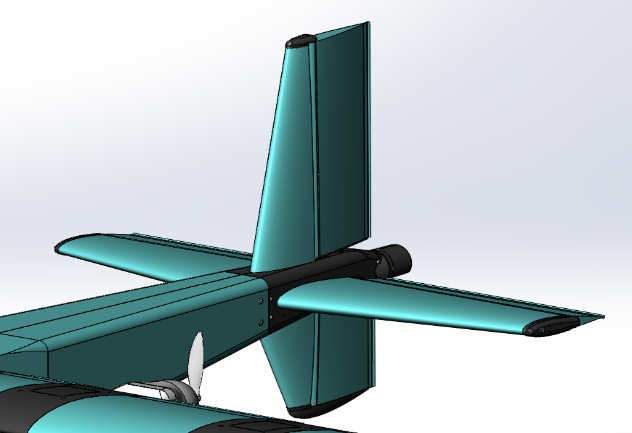
\includegraphics[width=\textwidth]{resulting-tail-design}
        \caption{}
        \label{fig:final-tail-design:angle}
    \end{subfigure}
    \hfill
    \begin{subfigure}[b]{0.49\columnwidth}
        \centering
        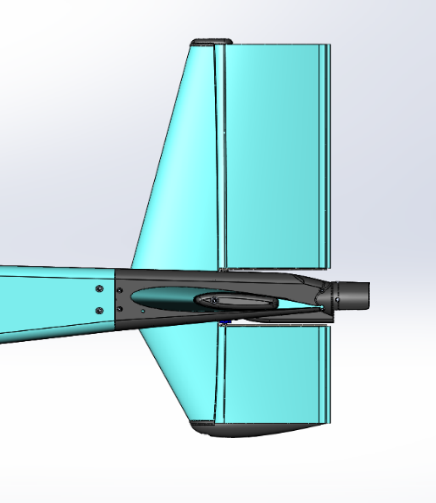
\includegraphics[width=\textwidth]{resulting-tail-design-side}
        \caption{}
        \label{fig:final-tail-design:side}
    \end{subfigure}
    
    \caption{resulting tail design.}
    \label{fig:final-tail-design}
\end{figure} 

One verification was to calculate the pitch stability derivative, using equation 6.67 in (Sadraey, 2013), which resulted as -0.6301.
A negative value indicates that the pitch moment decreases with alpha, which is desirable.
Following a process from Aerospace course year 2 notes from Mechanics of Flight gave a stick fixed static margin of 0.1574, and a stick fixed manoeuvre margin of 0.2747, both of which are acceptable values (De-Kat, 2017). 

Work on the yaw control requirements of the aircraft led to the decision to have an upper and lower vertical stabiliser, since extra rudder area was required, and to act as a bumper so that that in tail pusher propeller configuration, where take off rotation or a hard landing might lead to tail propeller contacting the ground, the propeller and therefore the aircraft would be protected.
It was considered to mount a wheel on this bumper when thought to use a tail wheel configuration, however the team eventually settled on a nose wheel configuration, so the bumper remained (visible in figure 49 above). 

Tail spars were resized using the same process as the wind tunnel model, as it had been decided to switch to pultruded carbon fibre rather than aluminium to save weight and move the centre of gravity forward.
The process does not account for the bonding of the extra foam material to the spars, so the estimated deflection will likely be pessimistic.  

Basic calculations from Year 3 Aircraft Structural Design module (Bresloff, 2018) were made to assess the potential effect of gusts and manoeuvres on tail loading.
It was estimated that the maximum load likely to be seen in a gust encounter at the predicted flight altitude was approximately 39 N.
The maximum expected load from a manoeuvre was approximately 14 N, both within the 10g limit load designed for. 

\subsubsection{CAD modelling} \label{sec:design-process:final-design-proposal:tail:cad-modelling}

The tail surface CAD was generated as a lofted base using aerofoil profiles of a NACA0012 with a scaling factor applied to make a NACA0018, lining up at the trailing edge.
The root was shortened to allow for the tail mount geometry, and cut-outs added for the tail spars, control surfaces and hot wire routes.
Initially the control surfaces were to be pinned into place with a laser cut sheet bonded to the end of the lifting surface holding a pin extending into control surface for it to rotate around, however in order to facilitate disassembly of the tail sub-assembly, this was changed into a 3D printed component that would neatly hold a nut on the end of a threaded rod bonded to the end of the tail spar.

The tail surfaces were designed to be inserted into 3D printed component as it was realised that the tail would require a lot of functionality that would be hard to facilitate with a foam or set of laser cut parts.
This was decided to be a piece that would split in half vertically, allowing the vertical surfaces to be inserted easily, and the horizontal surfaces would require a small amount of trimming to allow them to slide in over the spars, and then secured using bolts.
The CAD process for the final version of the tail mount can be seen below:

% \importimage{tail-mount-one}{tail mount design, version one.}{Tail mount version one}{0.3}
% \importimage{tail-mount-two}{tail mount design, version two.}{Tail mount version two}{0.3}
% \importimage{tail-mount-three}{tail mount design, version three.}{Tail mount version three}{0.3}

\begin{figure}[H]
    \centering
    \begin{subfigure}[b]{0.32\columnwidth}
        \centering
        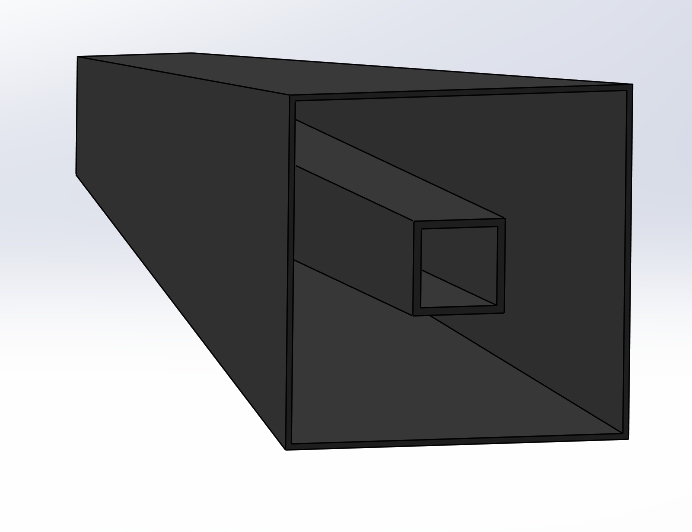
\includegraphics[width=\textwidth]{tail-mount-one}
        \caption{}
        \label{fig:tail-mount-progression:initial}
    \end{subfigure}
    \hfill
    \begin{subfigure}[b]{0.32\columnwidth}
        \centering
        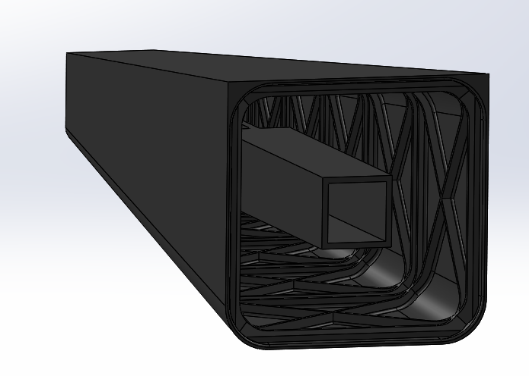
\includegraphics[width=\textwidth]{tail-mount-two}
        \caption{}
        \label{fig:tail-mount-progression:revised}
    \end{subfigure}
    \hfill
    \begin{subfigure}[b]{0.32\columnwidth}
        \centering
        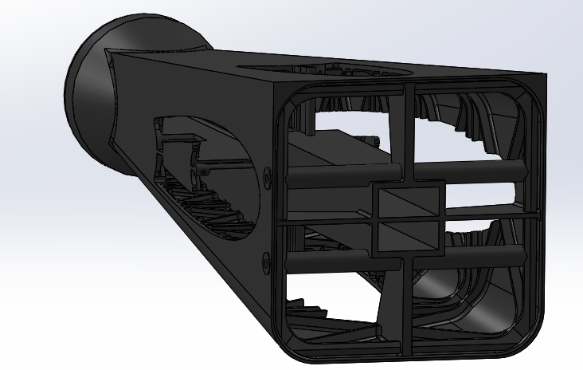
\includegraphics[width=\textwidth]{tail-mount-three}
        \caption{}
        \label{fig:tail-mount-progression:final}
    \end{subfigure}
    
    \caption{progressive iterations of the tail mount design.}
    \label{fig:tail-mount-progression}
\end{figure} 

The process began with a tapered section hollowed out to 1.5 mm wall thickness, and a rectangular tube added for the tail spar.
The inside and outside corners were filleted. 

Next ribs were added for lightweight structural support, made by a complex series of combined bodies.  

Supporting structure was added from the outside walls to meet the spar tube in the centre.
A mounting location was added for the tail motor, and channels to run securing bolts through added, as it was planned to make the part in two halves to aid assembly.  

In an assembly, the tail lifting surfaces were added, and moved to the correct position using mates, and then their bodies subtracted from the mount body. 

Servo mounts were added and a motor mounting solution added based on a teammates previous design, and then a shroud was added over the motor, as well as a wire route for the motor connections.
The structure was eventually split in half and holes for spars added, and the model tidied up for 3D printing. 

A small structure was added to the front to allow for mounting to the foam ahead of it 

Finally a small 3D printed part was designed to fit into the attachment location at the rear of the tail mount.
This was based on Michael Pywell’s design earlier on in the project, and simply had a cylinder with wide radial teeth protruding from the inside.
The motor mount had the same teeth, and would slide axially in the cylinder through the gaps, and then rotate, the teeth overlapping to prevent the mount from moving.
Small holes cut through both parts of the mount allowed for threaded inserts to be placed inside, and then screws through the same holes would secure the mount in place. 

% \importimage{tail-mount-slice}{a view of one half of the final tail mount.}{Tail mount slice}{0.4}
% \importimage{tail-mount-final}{a view of the final tail mount design.}{Tail mount design}{0.4}

\begin{figure}[H]
    \centering
    \begin{subfigure}[b]{0.49\columnwidth}
        \centering
        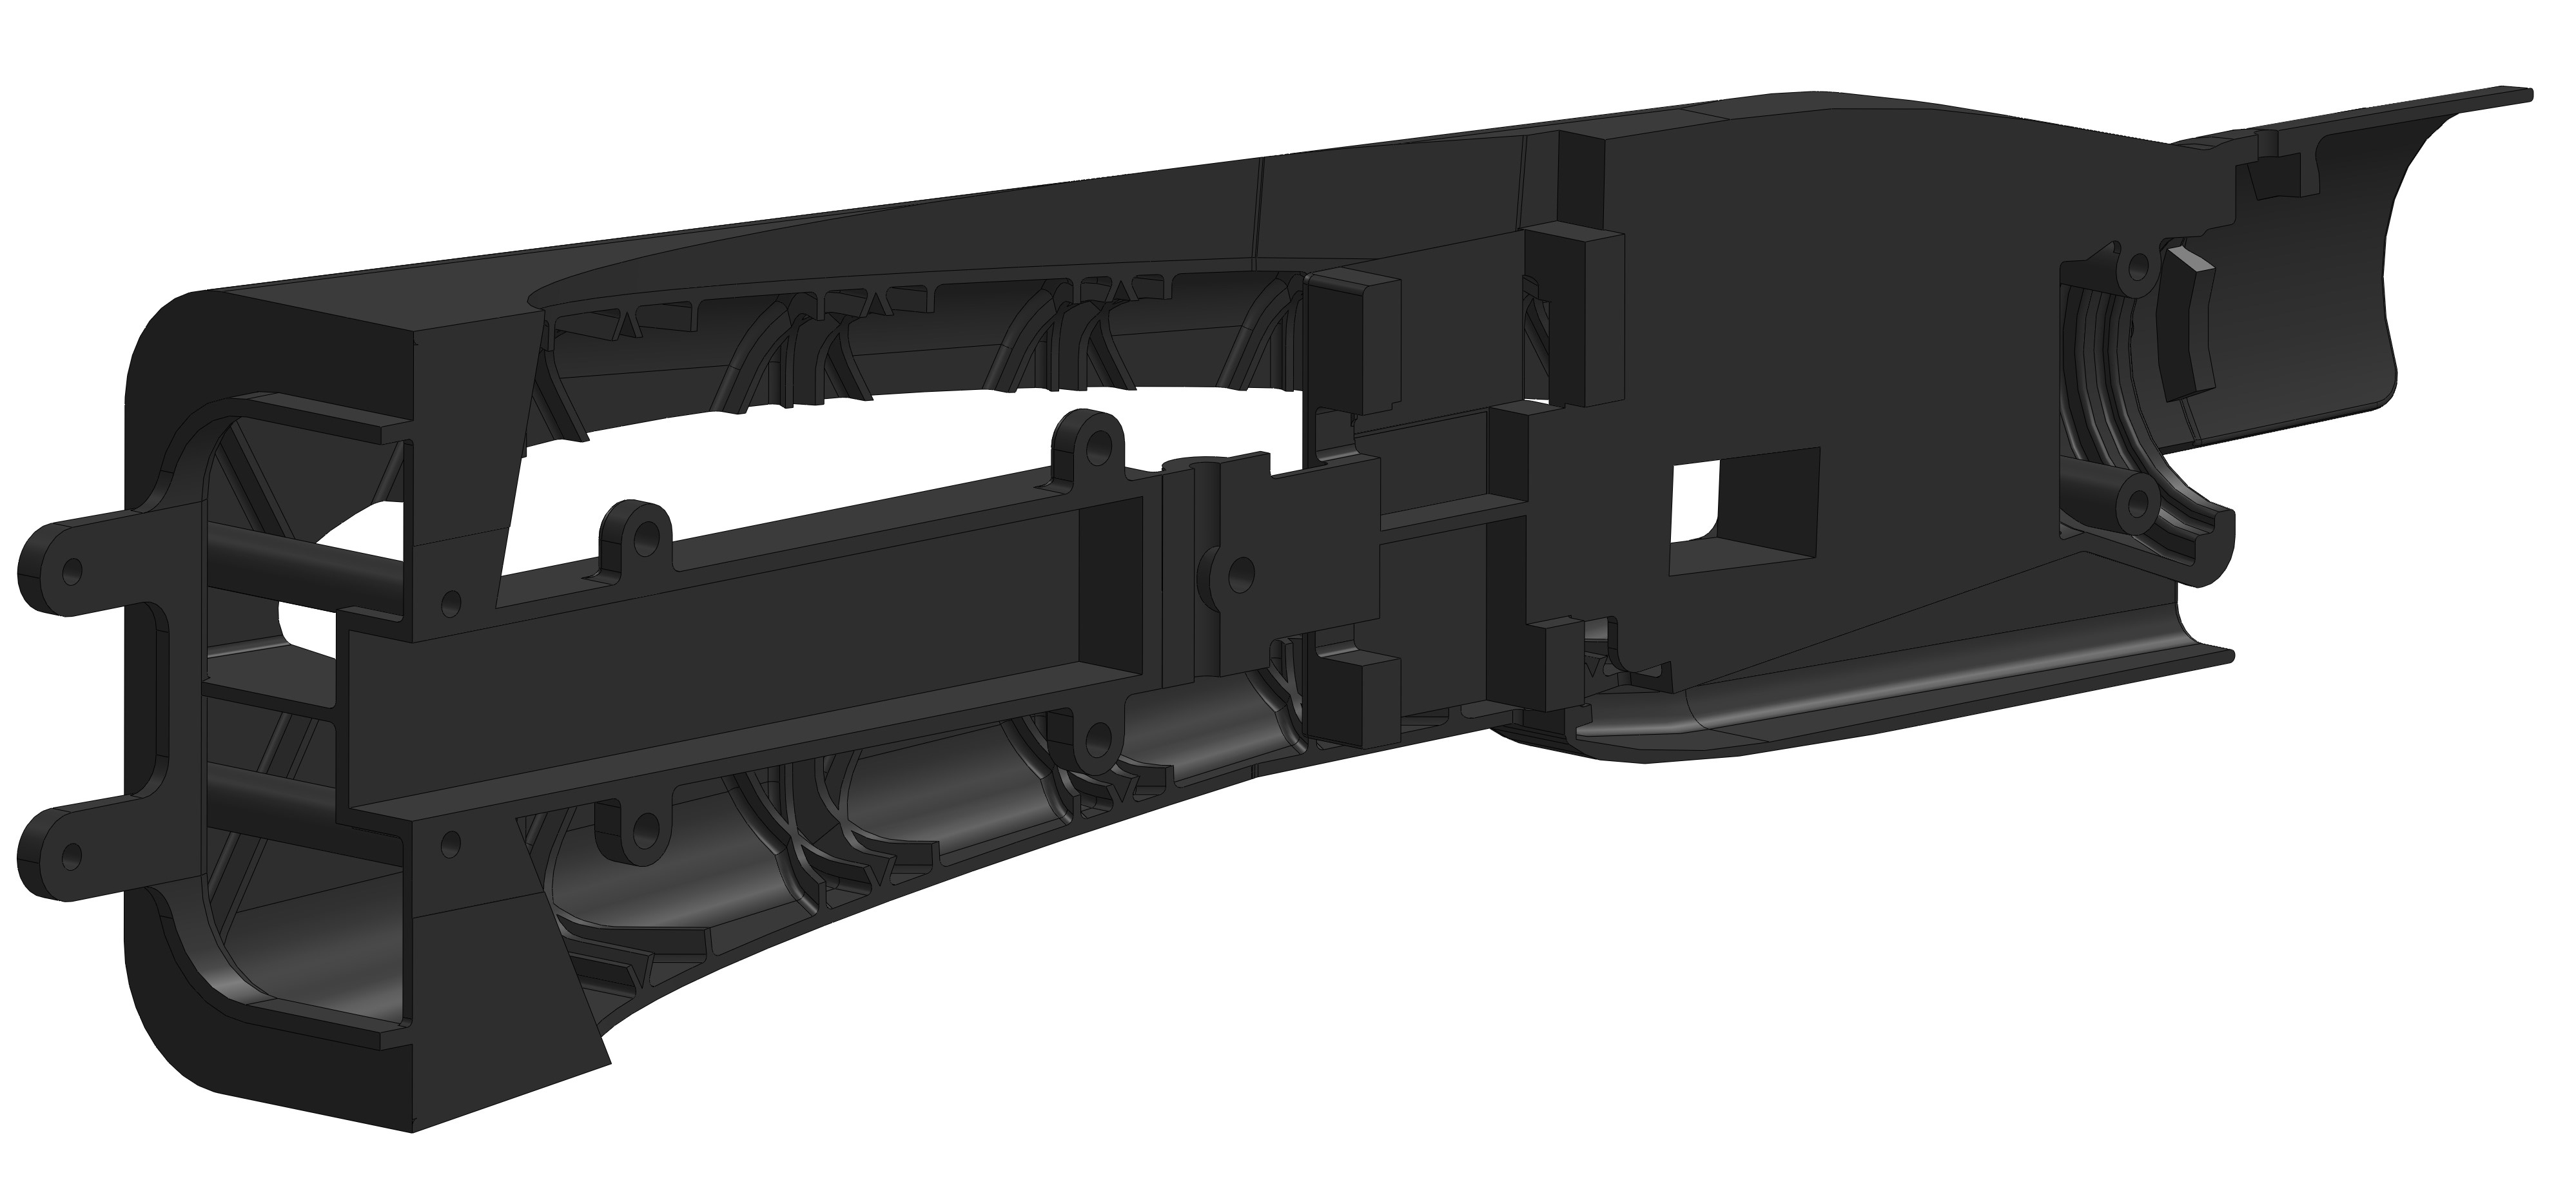
\includegraphics[width=\textwidth]{tail-mount-slice}
        \caption{}
        \label{fig:tail-mount-design:slice}
    \end{subfigure}
    \hfill
    \begin{subfigure}[b]{0.49\columnwidth}
        \centering
        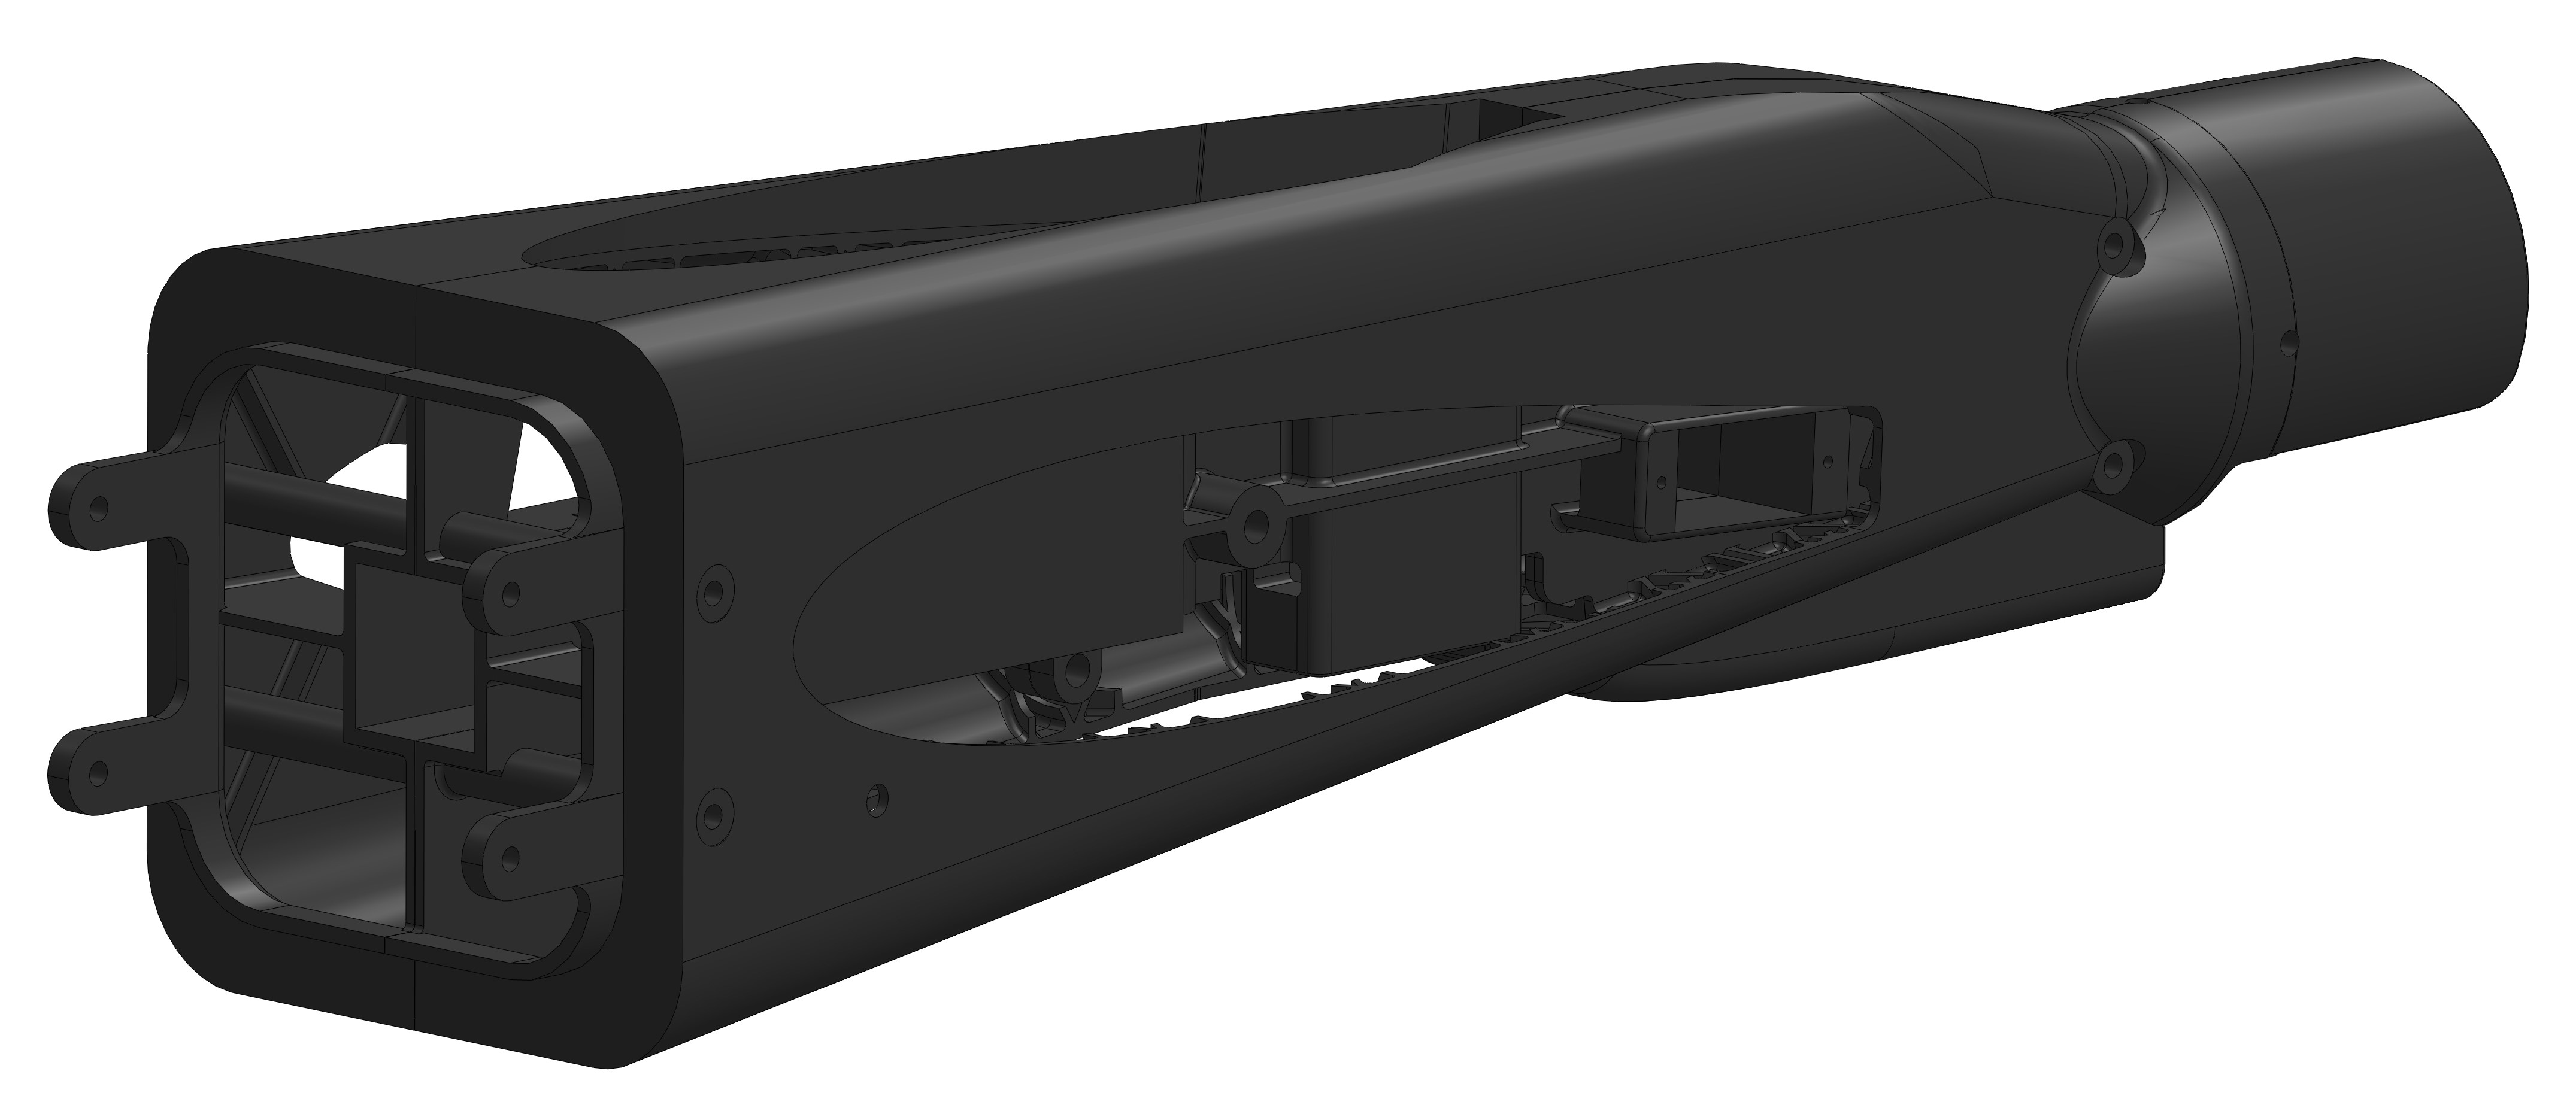
\includegraphics[width=\textwidth]{tail-mount-final}
        \caption{}
        \label{fig:tail-mount-design:whole}
    \end{subfigure}
    
    \caption{final tail mount design; (a) shows a cut view.}
    \label{fig:tail-mount-design}
\end{figure} 

\importimage{exploded-tail}{exploded view of the tail assembly, including fasteners.}{Exploded tail assembly}{0.7}

\subsection{Control surfaces} \label{sec:design-process:final-design-proposal:control-surfaces}

\subsubsection{Mathematical modelling} \label{sec:design-process:final-design-proposal:control-surfaces:mathematical-modelling}

The control surfaces were designed around their ability to meet several criteria that commercial aircraft must satisfy to be flyable. While this UAV isn’t required to meet the same stringent safety standards, many are there simply to ensure the aircraft flies properly, so it was prudent to meet them, a such, the rudder was designed to maintain trim control in the unlikely event of a wing tip motor failing resulting in worst case asymmetric thrust.  

To begin, the rudder was parameterised in terms of the ratio of it’s chord to the root chord of the vertical stabiliser, it’s span, and it’s inside offset from the root of the stabiliser allowing space for the servo.
Several useful parameters were derived from this including the MAC ratio, which was used on a plot from (Sadraey, 2013) to find the angle of attack effectiveness ($tau$) of the rudder, which was used to calculate the rudder control derivative using equation 12.100 in (Sadraey, 2013).
The rudder was modelled to be functioning at the predicted stall speed of the aircraft as it would be expected to maintain control at this speed.
A maximum deflection of 30 degrees was selected based (Sadraey, 2013), then this and relevant values substituted into equation 12.104a in (Sadraey, 2013) to calculate the vertical stabiliser lift with a deflected rudder. 

The first version of this with only the upper vertical stabiliser yielded a lift of 5.08 N.
This required comparing to the moment from the tip motor at full thrust, at stall speed.
The thrust of the motor changes with the inflow velocity.
Analysis of motor test data gave the thrust at predicted stall speed to be 8.73 N.
The wing has a semi-span of 1 m, so this is equal to the moment theoretically created in an asymmetric thrust scenario at this speed.
The tail arm was initially to be 1 m, but was reduced to 0.9 m for the purpose of moving the centre of mass forward, giving a tail moment of 4.57 Nm, which is approximately half of that required by the asymmetric thrust scenario.
This design flaw, combined with the fact that the rear propeller in that configuration would be unprotected on rotation or a hard landing, led to the decision to add a lower vertical stabiliser, despite it being surplus required vertical stabiliser area. 

The upper stabiliser was extended very slightly, the same root and tip chords maintained for upper and lower stabilisers, and simply a span extended below the fuselage until it extended approximately an inch beyond the lowest reach of the rear propeller, visible in figure 53. 

The values of both spans were altered until the force created by the deflected rudder was sufficient to counteract the moment from the asymmetric thrust.
The increase of the span had the effect of increasing the effective aspect ratio of the vertical stabiliser, which increased the efficiency, and thus the 3D lift curve slope, so it wasn’t required to simply double the area. 

The calculation was run with different speed values in Excel, to plot the rudder effectiveness and the motor thrust moment, over the expected speed range of the UAV: 

\importimage{rudder-thrust-moment}{rudder against thrust moment at various speeds.}{Rudder against thrust moment}{0.95}

With this requirement satisfied, design of the rudder was concluded.
The lack of runway landing and already excessive rudder size lead to the decision to forgo other rudder validation tests. 

The next stage of the design was the elevators, which began with parameterized geometry of the elevator through a root chord ratio.
A value of a quarter chord was selected initially, and this proved to be more than sufficient for all subsequent analyses, so remained.
The elevators took up all available trailing edge span of the horizontal stabiliser, leaving only room for the servo required to control it.  

The first attempt at the analysis of required deflections implemented a MATLAB code from (Sadraey, 2013) section 12.8.2, in Excel, to plot out the elevator deflections for the most fore and aft centre of gravity, and over the predicted speed range of the UAV.
The output of this code appeared to not be able to capture the 0 elevator deflection required at cruise speed (as the tail mounting angle has been designed around this).
Prof. Towell provided another method to try before assuming that the tail mounting angle calculations were wrong.  

The process given started with a moment balance about the centre of gravity of the aircraft including lift, tail lift, wing pitch moment equated to the tail lift moment.
This could have values substituted in for lift, and be rearranged for the tail lift coefficient: 

\importequation{
    C_{L_h} = \frac{q S C_L (h-h_0) c + T z_T + q S C_{M_0}}{q S_h l}
}{cog-moment-balance}

Then performing analysis of forces in vertical equilibrium, rearranging and substituting for the tail lift coefficient above  and rearranging for alpha, yielded the fuselage angle of attack at a given cruise condition: 

\importequation{
    \alpha = \frac{2 (mgl - Tz_T) V^{-2} - c C_{M_0}}{\rho S C_{L_\alpha}(l + (h - h_0)c)}
}{vertical-equilibrium}

With alpha found for a range of speeds, it could be used to find the tail lift coefficient for that particular speed, which is found by a rearranged version of the equation for tail lift coefficient, noting $\frac{S_h l}{Sc} = \overline{V}_h$, yielding: 

\importequation{
    C_{L_h} = \frac{C_{L_\alpha}\alpha(h-h_0) + \frac{Tz_T}{qSc} + C_{M_0}}{\overline{V}_h}
}{rearranged-tail-lift-coefficient}

With this, the elevator deflection can finally be calculated using:

\importequation{
    \delta = \frac{C_{L_h}}{C_{L_{\alpha_h}}} - \alpha (1 - \epsilon_\alpha) - \epsilon_0 - \frac{\alpha_h}{\tau_e}
}{elevator-deflection}

The process used above, along with the failed MATLAB code, repeated for a range of speeds yielded this plot (see legend for details):

\importimage{elevator-deflection}{elevator deflection plots for both processes.}{Elevator deflection plots}{0.95}

The second process captured the 0 deflection required at cruise speed, and appeared to be correct, so design was concluded as satisfactory in this case.
Additionally the deflections required from below the stall (and take off) speed are within the maximum deflections of the elevator selected.
The last test for the elevator was that it was satisfactory for aircraft rotation performance, which was based on a process from section 12.8.2 in (Sadraey, 2013), and involved determining all forces and moments on the aircraft for the elevator to overcome on aircraft rotation.
To begin, the take-off induced drag factor was determined using equation 5.22 in (Sadraey, 2013), then this and other pre-determined values were used to determine the take-off drag coefficient using equation 5.68 from (Sadraey, 2013).
This was then used to determine the take-off drag using the basic drag equation at a take-off speed of 13 m s-1 and a value of 11.56 N was calculated.  

Next the pitching moment about the aerodynamic centre was estimated as the wing 0 lift pitch moment coefficient, and then a basic pitch moment equation to determine the moment on take-off as -2.55 Nm.
The aircraft’s linear acceleration on rotation was then determined using equation 12.55 from (Sadraey, 2013) with an estimated friction coefficient of grass from Table 9.7 in (Sadraey, 2013). 

Next, several geometric parameters of the aircraft were determined from the CAD model to be then substituted into equation 12.72 in (Sadraey, 2013) to determine the lift required of the tail to achieve a set angular acceleration given the aircraft’s mass moment inertia about the pitch axis.
This yielded a tail lift of -3.17 N, which gave a tail lift coefficient of -0.192.
Checking using the method defined previously to determine the elevator deflections at various speeds gave+ a required deflection of -7.59o, which is less than the maximum of -25o, so this is acceptable.
This concluded elevator design. 

Finally, the ailerons required sizing.
This was based around their ability to reach a required roll angle within a set time.
This requirement varies based on the aircraft type and flight phase, which was determined from table 12.12b in (Sadraey, 2013) as a class II at phase C, at level 1.
The ailerons were parameterized by chord ratio (beginning with a value of 0.25, which proved satisfactory, so remained), and their inboard and outboard spans, however these were limited by the motor mount locations, so the main value to iterate upon was the chord ratio.  

A process from section 12.8.1 of (Sadraey, 2013) was used to determine aileron performance, beginning with the determination of the angle of attack effectiveness of the ailerons using the same method as previously.
This and several parameters were used in equation 12.23 from (Sadraey, 2013) to determine the aileron rolling moment coefficient derivative, yielding a value of 0.273 rad s-1, which was then used to determine the aileron rolling moment coefficient at the maximum deflection of the aileron using equation 12.13 in (Sadraey, 2013), which gave a value of 0.095. 

The ailerons need to be effective at an estimated approach velocity of 1.1 times the stall speed.
The aileron lift was then determined using equation 12.11 in (Sadraey, 2013) which resulted as 10.04 N.
This was then used to determine the steady state roll rate using equation 12.37 in (Sadraey, 2013), which gave a value of 7.14 rad s-1, which was then used to determine the bank angle at which the steady state roll rate would be achieved, using equation 12.43 in (Sadraey, 2013), which gave a value of 74.57 degrees.
The rate of roll rate could then be calculated using equation 12.49 in (Sadraey, 2013), which gave a value of 0.342 rad s-2.
Finally, the time to reach a bank angle of 30 degrees could be calculated using equation 12.47 in (Sadraey, 2013), which resulted as 1.75 seconds, less than the maximum 1.8 seconds, so the aircraft satisfied roll control requirements.
The time reduced to 1.17 seconds for the same process repeated at cruise speed. 

To conclude control surface mathematical design, it was checked using XFOIL that the servos chosen would be able to cope with the hinge moments.
For aesthetics it was chosen to have the servo axis in line with the control surface axis.
This removes the need for horn controls.
A code was used that yielded a hinge moment coefficient, which was then multiplied by relevant values to obtain the hinge moment.
As the servo and control surface axes were in line, if this value was greater than the stall torque of the servo, the servo was deemed inappropriate.
The SG90S had been selected, and was appropriate for all control surfaces, apart from the upper rudder, which was later changed to a HITEC HS 85 MG servo, which had sufficient stall torque. 

\subsubsection{CAD modelling} \label{sec:design-process:final-design-proposal:control-surfaces:cad-modelling}

% \importimage{elevator}{a single elevator.}{Elevator}{0.4}
% \importimage{transparent-stabiliser}{a transparent view of the assembly of one horizontal stabiliser and elevator.}{Horizontal stabiliser}{0.4}

\begin{figure}[H]

    \centering
    \begin{subfigure}[b]{0.49\columnwidth}
        \centering
        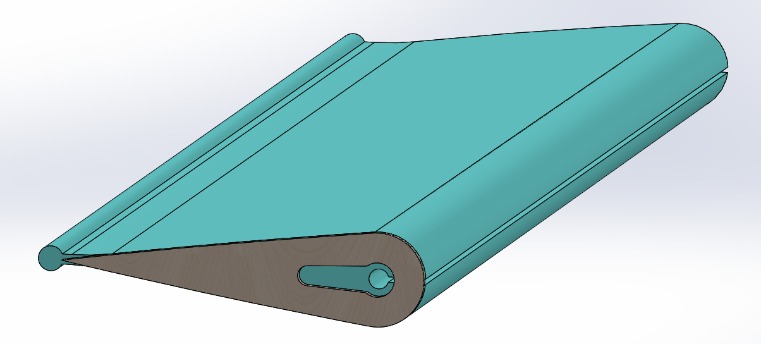
\includegraphics[width=\textwidth]{elevator}
        \caption{Elevator}
        \label{fig:tail-assembly:elevator}
    \end{subfigure}
    \hfill
    \begin{subfigure}[b]{0.49\columnwidth}
        \centering
        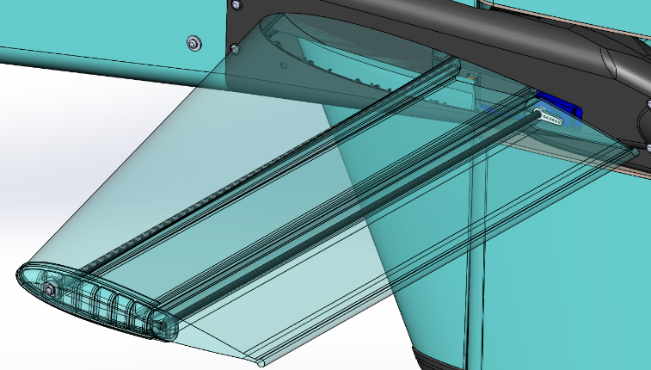
\includegraphics[width=\textwidth]{transparent-stabiliser}
        \caption{Horizontal stabiliser}
        \label{fig:tail-assembly:horizontal-stabiliser}
    \end{subfigure}
    
    \caption{components of the horizontal component of the tail section.}
    \label{fig:tail-assembly}
\end{figure} 

The rudder basic shape was cut out from a duplicate of the vertical stabiliser model.
The space for the servo was cut out from the root, then additional cut-outs made for the stiffening spar near the leading edge, and foam cutter wire paths.
Next a thin second body was extruded from the root to define a laser cut profile that would allow for the servo arm to have a place to nest into, allowing for control of the rudder.
Lastly a small circular profile (designed to be cut off manually later) was extruded on the trailing edge so that the foam cutter would not damage the trailing edge since it was so thin.
The secondary rudder and elevators were defined identically. 

The ailerons were generated from a sketch of the aerofoil profile which was defined from the wing profile sketch, then one aileron extruded in a long profile, then, planes were defined in the model that referenced the motor mount surfaces in contact with the aileron root and tip surfaces.
Material outside of these two planes was then removed to define one aileron, which was then mirrored about the centre plane, defining both ailerons in a way that would instantly react to changes in motor mount location and spans between them.
Next a small amount was cut off the roots of the ailerons and replaced with a small laser cut profile extruded outwards, similarly to the tail control surfaces that allowed for the inline servo arm to control the aileron.
Finally, holes were added for a stiffening spar, and wire paths added for the foam cutter. 

\subsection{Electronics} \label{sec:design-process:final-design-proposal:electronics}

% TODO: split into subsubsections

The avionics of the aircraft were meant to fulfil two main goals.

\begin{itemize}
    \item Provide the pilot with assistance in flying the aircraft using a flight controller, generally maintaining stability. 
    \item Have basic autopilot functionality, allowing the aircraft to fly in straight and level flight at a consistent speed to enable the fair testing of different flight configurations. 
\end{itemize}

As well as this, the avionics would be required to extend and retract the flaps, and ideally to record data - specifically on the rate of battery drainage. 

The primary role of the flight controller is to convert control inputs from the pilot into control inputs that are sent directly to the servos, and is normally accomplished through a range of techniques, including PID controllers.
Two main flight controllers were investigated, the first being a Pixhawk flight controller - more expensive, but potentially more useful and had been used by people at the university before - and the second being a Matek F405-Wing board with iNav Flight firmware installed on it. 

While the Pixhawk could have been easier to set up, with its advertised “plug and play” functionality, it was significantly more expensive, and it was decided that looking into the Matek controller could be worth a potentially large saving, albeit with a greater risk of purchasing the controller to find that it did not work as expected.
The Matek hardware came at about half the cost, and while the corresponding firmware was relatively immature, its open source nature meant that its functionality was expanding quickly, and it had favourable reviews from a number of online sources.
Another potential advantage of the Matek controller was that it was designed specifically with fixed wing aircraft in mind, whereas the Pixhawk was focused more towards quadcopters. 

\importimage{matek}{pin layout and documentation for the Matek flight controller.}{Flight controller layout}{0.95}  % TODO: include source (http://www.mateksys.com/?portfolio=f405-wing)

Other beneficial features of the Matek board were the built-in current sensor and inertial measurement unit (IMU) which would provide estimates of the position, and more importantly orientation, of the UAV.
There were also a number of fairly low-cost GPS and airspeed sensor units, required for the latter part of the avionics system’s brief of providing autopilot functionality. 

\importimage{flight-configurator}{flight configurator software used to set up the flight controller.}{Flight configurator}{0.6}

Input to the flight controller could be achieved through a number of systems, most notably through SBUS; this type of serial connection appeared to be the most commonly supported amongst receivers, and would allow up to sixteen channels to be passed from the receiver to the controller.
The minimum required channels would be eight: four for throttle, yaw, pitch, and roll; two for flaps (on/off); and similarly two for the autopilot toggle.
With the additional channels it would in principle be feasible to implement extra features, such as manually cutting off outboard motors in the event that one of them should fail. 

Also of interest were the UART ports, which is a serial communication protocol broadly compatible with a number of microcontrollers, including Arduinos.
This would be a good option for extracting the data from the current sensor and passing it to a microcontroller - most likely an Arduino Nano - which could then integrate the current draw over time to provide an estimate of the battery capacity used by a particular configuration.
Being able to do this onboard was appealing because the need for telemetry, which would have significantly increased the complexity of the radio system, could be removed.
All data could be logged by a relatively simple program, written in C++, which could then be downloaded after each flight. 

\importimage{flight-controller-computer}{flight controller plugged into a computer running the flight configurator.}{Flight controller configuration}{0.6}
\importimage{flight-controller-receiver}{receiver undergoing the binding procedure.}{Receiver binding}{0.5}

While a Futaba transmitter was originally to be loaned from the university, scheduling constraints resulted in its unavailability for the duration of the project.
As an alternative, a FrSky Taranis X9D was purchased upon recommendation of its being a good tradeoff between price and flexibility.
The model is widely used and compatible with a wide range of receivers, uses a standard communication protocol, and also runs a configurable operating system, OpenTx, which enables it to be programmed in Lua.
As well as the standard joysticks, the handset has triggers and switches which can be mapped to the flaps and autopilot channels. 

Two primary factors constrained the selection of receiver.
The first was the output method, which needed to be SBUS to be compatible with the Matek flight controller, and have at least eight output channels.
The second was compatibility with the Taranis transmitter, which ruled out a number of Futaba receivers operating on a proprietary communication protocol. 

Other factors, while less important, included the power usage, cost, and size of the receiver.
The receiver was intended to fit onto an electronics tray along with the flight controller, and would be powered by the same battery as the flight controller, microcontroller, and servos.
A receiver, the FrSky X8R, was found, operating on 100mA at 5V (the standardised output voltage of the flight controller), and weighing less than 20g.
Its profile is also similar to that of the flight controller, meaning that it would not be the limiting factor in the size and shape of the electronics tray when the fuselage was designed. 

When bound to a Taranis X9D, the X8R is capable of receiving sixteen independent channels via FrSky’s radio transfer protocol ACCESS (a newer and more robust version of ACCST).
This would be more than sufficient for the eight channels required as a baseline for the project, and would also leave room for the expansion of the project with additional features, as mentioned previously, with the eight leftover channels.
The operating range of 1.5km would also be more than sufficient for the project. 

As well as being compatible with the Taranis transmitter and capable of outputting to SBUS, the receiver had a number of serial ports (standard PWM outputs) which could be used for testing and validating its functionality without having to pass the signals through the flight controller first.
It was thought that this could be useful in the later stages of the project while troubleshooting any issues, being able to remove the flight controller from the loop and isolate the receiver to check that it was communicating properly with the transmitter. 

All moveable surfaces on the aircraft are actuated by servos.
These are split into four groups: ailerons, elevators, rudder, and flaps.
The first three are the control surfaces by which the aircraft is controlled, and would need to be sized for a fairly limited selection of manoeuvres.
It was not expected that the aircraft would be performing any tight turns, but the load that would be transferred through the aileron servos could depend greatly on the configuration of the propulsion modules.
With the modules located at the end of the wings, the greatly increased moment of inertia of the aircraft would mean that actuating the ailerons would not produce nearly as much inertial relief as when the motors and batteries were located on the centreline.
As such, the servos could be expected to see a fairly variable range of loads.
In addition, the loads experienced by the rudder servos was found to be far in excess of the loads experienced by all other servos when the possibility of an asymmetric motor failure at the wingtips was considered.
It was decided that these servos would need to be of a different type to those elsewhere in the aircraft. 

In all, fourteen servos would be required to control the aircraft, including the two servos of different specification for the rudder.
The exact configuration of these servos, as well as the signals passed to each of them, is shown below. 

\importimage{signal-splitters}{control signal splitter schematic.}{Signal splitter schematic}{0.7}

Note that each flap is supported by two servos of opposing deflection directions.
While the flaps increase the lift of the aircraft quite dramatically, and thereby exert a large moment onto their supporting servos, the distribution of this load across four flap segments and eight servos meant that the smaller servo size was capable of holding the flaps in place during takeoff and landing. 

One potential issue with the servos selected was the degradation of the plastic-toothed gears they use.
Information from peers suggested that sufficient use would wear the gears down and reduce their effective strength, causing the gears to slide at a smaller load than suggested by the servos’ data sheets.
An experiment was devised to repetitively test a servo under load (actuating it far more times than would ever be expected of a servo in a flight model) to see whether its strength afterwards was the same as upon its delivery; but this experiment was never carried out due to the COVID-19 pandemic.
In the event that it had been found to significantly impact the strength of the servos, metal-toothed servos could have been purchased at a slightly higher cost. 

The entirety of the electronics subsystem was to be powered by a single battery, referred to as the avionics battery.
This would be connected to the flight controller, powering it directly, and indirectly powering the receiver, microcontroller, and servos.
While throttle signals would be supplied to the motors from the flight controller directly, the bulk of their power would come from the ESCs, which are in turn powered by the battery local to that propulsion module. 

In order to size the battery used for the avionics, the approximate power draw of each of the electrical components needed to be determined.
Research was conducted, considering the following items drawing power during a typical 10-minute flight: 

\begin{itemize}
    \item Servos
        \begin{itemize}
            \item Draw 10mA while idle, 100-250mA while moving, and have a stall current of 360mA 
            \item The stall torque of the servos being used is 1.7kg.cm, meaning that for a 4cm control surface, a load of roughly 0.5kg would need to be applied to cause a stall.
                Considering that there are nine control surfaces and that the total lift generated by the aircraft is around 7kg, it can reasonably be assumed that the likelihood of any individual control surface experiencing a load of 0.5kg is extremely small; certainly small enough that it will occur only momentarily and does not need to be factored into the draw calculations 
            \item 8 servos are being used for the flaps and so will only move for a few seconds per flight 
            \item One servo connected to the nose gear, which will likely only be moving periodically within two 30-second windows at the start and end of each flight 
            \item 5 servos are connected to the control surfaces.
                It is assumed that control surfaces will only move for around 50\% of the time while in the air.
                To build in a bit of redundancy and account for the movement of the flap/gear servos, it is assumed that the power drain from servos will be equivalent to five servos moving constantly 
            \item This then means 1000mA drawn by servos 
        \end{itemize}
    \item Receiver: listed as drawing a continuous 100mA 
    \item Flight controller: listed as drawing a continuous 500mA, a conservative estimate 
    \item The exact current draw of a microcontroller is difficult to determine as it depends primarily on how much the processor is being used.
        Even conservative estimates resulted in around 20mA of draw, so that was neglected here as it is so much smaller than the other components 
\end{itemize}

An additional constraint placed on the battery was the required voltage of between 9 and 30 volts.  As the battery needs to be a LiPo battery, this limited the selection to those with between 3 and 6 cells. 

Given a total of 1600mA drawn while in flight (a conservative estimate which also accounts for the small amount of additional power used for one-off events during takeoff and landing), and the voltage requirements, a few batteries were found which could power the avionics.
Several higher-capacity batteries were heavier and more expensive and, while they would enable multiple flights on one battery, switching out multiple lower-capacity batteries which were both lighter and cheaper was found to be more cost- and mass-effective, and also in keeping with the modular nature of the project. 

The battery settled on was therefore a 450mA, 11.1V, and 65-130C discharge, which should provide for at least 15 minutes of flight on a conservative estimate of the power draw.
Its low cost means that multiple can be bought and swapped out between flights, while used batteries are recharged. 

With all the components of the avionics subsystem specified, a wiring diagram could be created and from this an iron bird constructed.
The primary goal of this exercise was to check that every required component was present, and that they would all fit together with the necessary wires. 

\importimage{wiring-diagram}{wiring diagram for the avionics subsystem.}{Wiring diagram}{0.6}

From the above diagram, the iron bird was built onto a miniaturised cutout of the same general shape as the full-size aircraft. 

\importimage{iron-bird}{iron bird.}{Iron bird}{0.7}

While not all of the servos were included in the iron bird, each servo group was represented.
The iron bird also gave a much clearer indication of roughly how much wiring would be needed to connect the various groups, and which layout would be most efficient for splitting the signals; that is, which signals should be brought down each of the main “limbs” of the aircraft, and where should they be split.
Once this was decided, the splitters could be designed and manufactured. 

\importimage{splitter-schematic}{manufacturing schematic for a single splitter.}{Manufacturing schematic}{0.5}

A schematic similar to the one shown above was drawn out for each of the splitters identified in Figure \ref{fig:splitter-schematic}.
This includes the specification of the splitter in terms of the signals designated as inputs and outputs, and shows its layout in terms of header pins (rectangular boxes) soldered (ovals) across a stripboard whose strips are assumed to go across the page horizontally.
Breaks in the stripboard are shown here by small vertical lines instead of a dot representing the corresponding hole. 

These splitters were manufactured from small cut segments of stripboard by simply soldering header pins in the correct locations.
The seven splitters also had small outcrops of stripboard so that they could be fastened to relevant locations throughout the body of the aircraft. 

\importimage{manufactured-splitters}{each of the manufactured splitters.}{Manufactured splitters}{0.8}

Although the full electronics system was never assembled in the UAV due to the COVID-19 pandemic, all of the necessary physical components were purchased and manufactured, and their compatibility was tested in the iron bird. 

% \importimage{electronics-housing}{render of the electronics housing bay in the tractor nose propulsion configuration.}{Electronics housing}{0.4}
% \importimage{electronics-exploded}{exploded view of the avionics subsystem.}{Avionics subsystem}{0.4}

\begin{figure}[H]
    \centering
    \begin{subfigure}[b]{0.49\columnwidth}
        \centering
        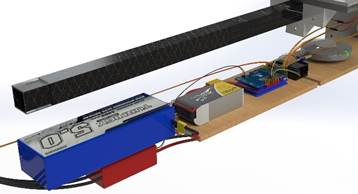
\includegraphics[width=\textwidth]{electronics-housing}
        \caption{Housing bay}
        \label{fig:electronics-subsystem:bay}
    \end{subfigure}
    \hfill
    \begin{subfigure}[b]{0.49\columnwidth}
        \centering
        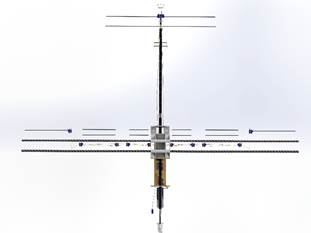
\includegraphics[width=\textwidth]{electronics-exploded}
        \caption{Subsystem, exploded}
        \label{fig:electronics-subsystem:exploded}
    \end{subfigure}
    
    \caption{renders of the key parts of the electronics subsystem.}
    \label{fig:electronics-subsystem}
\end{figure} 

\importimage{bixler}{image of the Bixler 3 RC plane.}{Bixler model}{0.5}

Before the electronics were to be flown on the UAV, they needed to be tested.
There was thorough testing of the electronics out of any aircraft first, but in order to be deemed flight worthy it needed to be tested in the air in a sacrificial flight vehicle.
The foamy selection was based on the constraints of the fuselage size required in order to have room to fit all of the electronics inside, keeping the cost as low as possible, and having an aircraft that we could fly ourselves (easy to fly for beginners).
The fuselage needed to be able to fit all of the necessity electronics; battery, ESC, receiver, as well as our additional electronics to control the autopilot; Arduino, Matek, and GPS.
Therefore we needed a beginners plane that had excess fuselage space, and so we chose the Bixler 3 as it has a large internal space for the necessity electronics, as well as an empty nose for installation of a camera for FPV flying, and this space would be suitable for fitting in our additional electronics.
Additionally the plane is designed for beginners and so has a large surface area wing for low speed flying, high mounted for flight stability, the motor and propeller face rearwards above the fuselage to get them out of the way of damage in the event of a crash, and the underside of the fuselage is strengthened to act as a skid if the landing gear comes off in a particularly heavy landing.
All of this makes it ideal for our use case.
However, it was not flow due to the coronavirus lockdown, and so the electronics could not be flight tested. 

\subsection{Avionics and software} \label{sec:design-process:final-design-proposal:avionics-and-software}

% TODO: populate from electronics section

\subsection{Propulsion} \label{sec:design-process:final-design-proposal:propulsion}

The design of the housing for the motors and its subsidiary systems focused on permitting the repositioning of these system in a small time window without the need for alteration to the design.
Thus increasing the amount of flights which can be completed in one day.
This was crucial so that the difference in atmospheric conditions are reduced to minimum. 
A self-contained housing storing the motor, the ESC and the battery was designed; referred as ‘Power Unit Cell’ (PUC).
The use of such design allowed the reduction of wires running through the wing as well as making those components more accessible for maintenance.
Furthermore, the use of a compact design allowed for a standard PUC which could be used in all wing propulsion configurations.
This was achieved by creating a standard simple profile for the surfaces normal to the attachment points; this is evident in Fig. 12.
In order to guarantee a smooth passage of the flow around the housing an adapter is created for each configuration.
This slots onto the standardized surfaces of the power unit cell and mounts directly on the wing surfaces blending the two together.
Furthermore, they ensure that the thrust line in unvaried between tractor and pusher configurations. 

% \importimage{puc-tractor}{PUC section view in top-tractor configuration.}{PUC top tractor}{0.5}
% \importimage{puc-pusher}{PUC section view in top-pusher configuration; yellow is the adaptor, green is the ESC, red is the battery, and blue is the motor.}{PUC top pusher}{0.5}

\begin{figure}[H]
    \centering
    \begin{subfigure}[b]{0.49\columnwidth}
        \centering
        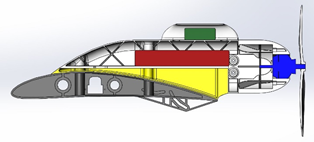
\includegraphics[width=\textwidth]{puc-pusher}
        \caption{Overwing pusher}
        \label{fig:puc-assemblies:pusher}
    \end{subfigure}
    \hfill
    \begin{subfigure}[b]{0.49\columnwidth}
        \centering
        \includegraphics[width=\textwidth]{puc-tractor}
        \caption{Overwing tractor}
        \label{fig:puc-assemblies:tractor}
    \end{subfigure}

    \begin{subfigure}[b]{0.7\columnwidth}
        \centering
        \includegraphics[width=\textwidth]{puc-exploded}
        \caption{Exploded}
        \label{fig:puc-assemblies:exploded}
    \end{subfigure}
    
    \caption{
        various views of the PUC assembly.
        Adapters are in yellow; ESCs are in green; batteries are in red; and motors are in blue.
    }
    \label{fig:puc-assemblies}
\end{figure} 

The distance from the trailing edge to the propeller in the pusher layout is equivalent to the distance from the leading edge to the propeller in the tractor layout.
Moreover, as in can be seen in Fig. 12.
The attachment holes for the mounting bolts remain in the same position despite the change in arrangement.
Hence, allowing to interchange propulsion layouts without the need of modifications to the components. 
The power unit cells are as well split in two components: a front section and a rear section.
Thus permitting to access the components stored inside with the removal of the four M4 bolts securing the two halves together.
Four threaded inserts imbedded in the nylon structure of the front section allow the fitting of the motor.
The battery and the ESC are instead slotted into the rear section of the cell.
The open section into which the ESC is placed ensures the cooling of this component in all configurations setup.
So to avoid common reliability issues caused by the overheating of this last.
An exploded view of the PUC assembly is shown in Fig. 13. 

% \importimage{puc-exploded}{exploded view of the PUC assembly.}{Exploded PUC}{0.6}

Due to the fitting of the battery and the ESC, the PUC assembly has a sensible weight.
In fact, as it will be discussed, the CG of the UAV is subject to a significant shift as the motor configuration is changed from tractor to pusher.
A reduction in this effect leads to a less significant need to rely on a ballast to maintain the CG in the same location. 
In order to reduce this effect, the battery was located in a closer position to half chord length with some compromises made for the aerodynamic aspect.
Furthermore, a work of light weighting of the components was carried.
Hence the use of ribs and reinforcements where loads concentrate and the use of thin walls shown in Fig. 14.
This resulted into an overall housing dry weight of 207g. 

% \importimage{puc-front}{PUC front section inner structure.}{PUC front section}{0.3}
% \importimage{puc-rear}{PUC rear section inner structure.}{PUC rear section}{0.3}

\begin{figure}[H]
    \centering
    \begin{subfigure}[b]{0.4\columnwidth}
        \centering
        \includegraphics[width=\textwidth]{puc-front}
        \caption{Front}
        \label{fig:puc-design:front}
    \end{subfigure}
    \hfill
    \begin{subfigure}[b]{0.4\columnwidth}
        \centering
        \includegraphics[width=\textwidth]{puc-rear}
        \caption{Rear}
        \label{fig:puc-design:rear}
    \end{subfigure}
    
    \caption{inner structure of the PUC.}
    \label{fig:puc-design}
\end{figure} 

\importimage{puc-printed}{PUC, printed in SLS nylon.}{SLS nylon PUC}{0.5}

\end{document}
